\documentclass[12pt,oneside,titlepage]{scrartcl} 

\newcommand{\myAutor}{Rico  (Matrikelnummer 12345)\\ \> \> \> 
Henning   (Matrikelnummer 12345)\\ \> \> \> 
Julian  (Matrikelnummer 12345)} % Autor
\newcommand{\myAdresse}{Stra\ss e 123 \\ \> \> \> 57xxx Siegerland} % Adresse
\newcommand{\myTitel}{Browser RPG-Adventure} % Titel der Arbeit
\newcommand{\myBetreuer}{Daniel Bitzer} % Betreuer
\newcommand{\myLehrveranstaltung}{Web Technologie} % Lehrveranstaltung
\newcommand{\myMatrikelNr}{123456} % Matrikelnummer
\newcommand{\myOrt}{Siegen} % Ort
\newcommand{\myAbgabeDatum}{\today} % Datum der Abgabe
\newcommand{\mySemesterZahl}{5} % Semesterzahl
\newcommand{\myHochschulName}{FOM Hochschule für Oekonomie \& Management Essen} % Name der Hochschule
\newcommand{\myHochschulStandort}{Siegen} % Standort der Hochschule
\newcommand{\myStudiengang}{Wirtschaftsinformatik} % Studiengang
\newcommand{\myThesisArt}{Projektdokumentation als Seminararbeit} % Art der Arbeit
\newcommand{\myAkademischerGrad}{Bachelor of Science (B. Sc.)} % Zu erlangender akademische Grad
\newcommand{\myFirma}{Mustermann GmbH} % Firma

\usepackage[ngerman]{babel}
\selectlanguage{ngerman}
\usepackage[babel,german=quotes]{csquotes}

\usepackage[utf8]{luainputenc}
\usepackage[T1]{fontenc}
\usepackage{fancyhdr}
\usepackage{fancybox}
\usepackage[a4paper, left=4cm, right=2cm, top=4cm, bottom=2cm]{geometry}
\usepackage{graphicx}
\usepackage{colortbl}
\usepackage[capposition=top]{floatrow}
\usepackage{array}
\usepackage{float}      %Positionierung von Abb. und Tabellen mit [H] erzwingen
\usepackage{footnote}
\usepackage[singlelinecheck=false, labelfont=bf, font=bf]{caption} % Tabellendesign lt. Leitfaden
\usepackage{caption}
\usepackage{enumitem}
\usepackage{amssymb}
\usepackage{mathptmx}
\usepackage[scaled=0.9]{helvet} 
\usepackage{courier}
\usepackage{amsmath}
\usepackage[table]{xcolor}
\usepackage{marvosym}			% Verwendung von Symbolen, z.B. perfektes Eurozeichen
\usepackage[colorlinks=true,linkcolor=black]{hyperref}
\definecolor{darkblack}{rgb}{0,0,0}
\hypersetup{colorlinks=true, breaklinks=true, linkcolor=darkblack, menucolor=darkblack, urlcolor=darkblack}
\renewcommand\familydefault{\sfdefault}
\usepackage{ragged2e}

\usepackage[hang, multiple]{footmisc} % Mehrere Fussnoten nacheinander mit Komma separiert
\setlength{\footnotemargin}{1em}

%\usepackage{todonotes} % todo Aufgaben als Kommentare verfassen für verschiedene Editoren

\usepackage{epstopdf} %Pakete für Tabellen
\usepackage{nicefrac} % Brüche
\usepackage{multirow}
\usepackage{rotating} % vertikal schreiben
\usepackage{mdwlist}
\usepackage{tabularx}% für breitenangabe

\definecolor{dunkelgrau}{rgb}{0.8,0.8,0.8}
\definecolor{hellgrau}{rgb}{0.0,0.7,0.99}
% Colors for listings
\definecolor{mauve}{rgb}{0.58,0,0.82}
\definecolor{dkgreen}{rgb}{0,0.6,0}

\usepackage{listings} % sauber formatierter Quelltext
% JavaScript als Sprache definieren:
\lstdefinelanguage{JavaScript}{
	keywords={break, super, case, extends, switch, catch, finally, for, const, function, try, continue, if, typeof, debugger, var, default, in, void, delete, instanceof, while, do, new, with, else, return, yield, enum, let, await},
	keywordstyle=\color{blue}\bfseries,
	ndkeywords={class, export, boolean, throw, implements, import, this, interface, package, private, protected, public, static},
	ndkeywordstyle=\color{darkgray}\bfseries,
	identifierstyle=\color{black},
	sensitive=false,
	comment=[l]{//},
	morecomment=[s]{/*}{*/},
	commentstyle=\color{purple}\ttfamily,
	stringstyle=\color{red}\ttfamily,
	morestring=[b]',
	morestring=[b]"
}

\lstset{
	%language=JavaScript,
	numbers=left,
	numberstyle=\tiny,
	numbersep=5pt,
	breaklines=true,
	showstringspaces=false,
	frame=l ,
	xleftmargin=5pt,
	xrightmargin=5pt,
	basicstyle=\ttfamily\scriptsize, 
	stepnumber=1,
	keywordstyle=\color{blue},          % keyword style
  	commentstyle=\color{dkgreen},       % comment style
  	stringstyle=\color{mauve}         % string literal style
}

\usepackage[
    style           = apa6, 
    uniquelist      = false,    
    maxcitenames    = 6,
    backend         = biber,
	urldate         = short,
	uniquename 		= true,
	language		= ngerman
	]{biblatex} 
		
	%% START Block für Funktion (1. Nennung von 2-6 Autoren: Alle Namen, danach nur noch 1. Name + et.al) 
	\usepackage{lmodern} 
	\makeatletter
	\newcommand{\apamaxcitenames}{6}
	\DeclareNameFormat{labelname}{%
	  \ifthenelse{\value{uniquelist}>1}
		{\numdef\cbx@min{\value{uniquelist}}}
		{\numdef\cbx@min{\value{minnames}}}%
	  \ifboolexpr{test {\ifnumcomp{\value{listcount}}{=}{1}}
				  or test {\ifnumcomp{\value{listtotal}}{=}{2}}}
		{\usebibmacro{labelname:doname}%
		  {\namepartfamily}%
		  {\namepartfamilyi}%
		  {\namepartgiven}%
		  {\namepartgiveni}%
		  {\namepartprefix}%
		  {\namepartprefixi}%
		  {\namepartsuffix}%
		  {\namepartsuffixi}}
		{\ifboolexpr{test {\ifnumcomp{\value{listtotal}}{>}{\apamaxcitenames}}
					 or test {\ifciteseen}}
		 {\ifnumcomp{\value{listcount}}{<}{\cbx@min + 1}
		   {\usebibmacro{labelname:doname}%
			 {\namepartfamily}%
			 {\namepartfamilyi}%
			 {\namepartgiven}%
			 {\namepartgiveni}%
			 {\namepartprefix}%
			 {\namepartprefixi}%
			 {\namepartsuffix}%
			 {\namepartsuffixi}}
		   {}%
		  \ifnumcomp{\value{listcount}}{=}{\cbx@min + 1}
			{\ifnumcomp{\value{listcount}}{<}{\value{listtotal}}
			  {\printdelim{andothersdelim}\bibstring{andothers}}
			  {\usebibmacro{labelname:doname}%
				{\namepartfamily}%
				{\namepartfamilyi}%
				{\namepartgiven}%
				{\namepartgiveni}%
				{\namepartprefix}%
				{\namepartprefixi}%
				{\namepartsuffix}%
				{\namepartsuffixi}}}
			{}%
		  \ifnumcomp{\value{listcount}}{>}{\cbx@min + 1}
		   {\relax}%
		   {}}%
		 {\usebibmacro{labelname:doname}%
		   {\namepartfamily}%
		   {\namepartfamilyi}%
		   {\namepartgiven}%
		   {\namepartgiveni}%
		   {\namepartprefix}%
		   {\namepartprefixi}%
		   {\namepartsuffix}%
		   {\namepartsuffixi}}}}
	\makeatother 
	\DeclareLanguageMapping{ngerman}{ngerman-apa}
	%% ENDE Block für Funktion (1. Nennung von 2-6 Autoren: Alle Namen, danach nur noch 1. Name + et.al)
	
	\DeclareDelimFormat*{finalnamedelim}{\addspace\bibstring{and}\space} % In Parencite von "&" auf "und" ändern
	\hypersetup{hidelinks}  %Grüne Links auf Literaturverz. unterdrücken.
	\setlength\bibitemsep{1.3ex} % Abstände im Literaturverzeichnis erhöhen
	\setlength\bibnamesep{1.0ex}
	\AtBeginBibliography{\singlespacing} % Zeilenabstand im Literaturverzeichnis ist Einzeilig - siehe Leitfaden S. 14
	\urlstyle{same} %Standard-Font für Link anstelle der "Schreibmaschinenschrift"
	\DeclareFieldFormat[misc]{urldate}{[#1\printfield{urldate}].} 	% Anpassung @online + @misc Bibl: Datum in eckigen Klammern ans Ende
	\DeclareFieldFormat[misc]{title}{\mkbibemph{#1}} %Anpassung @online + @misc Titel Kursiv	
	\DeclareFieldFormat[misc]{url}{Verfügbar unter\space \url{#1}} 	%Anpassung @online + @misc Text vor URL
	\renewbibmacro*{url+urldate}{\usebibmacro{url}\setunit{\addspace}\usebibmacro{urldate}}  % URL vor Abrufdatum setzen + getrennte Wörter "Verfügbar" und "Unter" entfernen
%%%% APA ENDE

\addbibresource{literatur.bib} %Bib-Datei einbinden
%\nocite{*} % Die folgende Zeile trägt ALLE Werke aus literatur.bib in das Verz. ein, auskommentieren um nur die anzuzeigen, die zitiert wurden


\usepackage{hyphsubst} %Silbentrennung
\HyphSubstIfExists{ngerman-x-latest}{%
\HyphSubstLet{ngerman}{ngerman-x-latest}}{}

\graphicspath{{./}{./media/}} % Pfad fuer Abbildungen

\usepackage{titletoc} % Weitere Ebene einfügen
\makeatletter

% Setze die Tiefe des Inhaltsverzeichnis auf 4 Ebenen -  Damit erscheinen \paragraph-Sektionen auch im Inhaltsverzeichnis
\setcounter{secnumdepth}{4}
\setcounter{tocdepth}{2}

% Fuege Abstand nach unten wie in einer normalen \section hinzu
\renewcommand{\paragraph}{%
  \@startsection{paragraph}{4}%
  {\z@}{3.25ex \@plus 1ex \@minus .2ex}{1.5ex plus 0.2ex}%
  {\normalfont\normalsize\bfseries\sffamily}%
}

\makeatother

\usepackage{appendix} % Paket für die Nutzung von Anhängen
\usepackage{setspace} % Zeilenabstand 1,5-zeilig
\onehalfspacing

\setlength{\parindent}{0mm} % Absätze durch eine neue Zeile
\setlength{\parskip}{0.8em plus 0.5em minus 0.3em}

\sloppy					%Abstände variieren
\pagestyle{headings}

\usepackage[printonlyused]{acronym} % Abkürzungsverzeichnis


% PDF Meta Daten setzen
\hypersetup{
    pdfinfo={
        Title={Browser RPG-Adventure},
        Subject={\myStudiengang},
        Author={\myAutor},
        Build=1.1
    }
}

% Umlaute in Code korrekt darstellen - siehe  https://en.wikibooks.org/wiki/LaTeX/Source_Code_Listings
\lstset{literate=
	{á}{{\'a}}1 {é}{{\'e}}1 {í}{{\'i}}1 {ó}{{\'o}}1 {ú}{{\'u}}1
	{Á}{{\'A}}1 {É}{{\'E}}1 {Í}{{\'I}}1 {Ó}{{\'O}}1 {Ú}{{\'U}}1
	{à}{{\`a}}1 {è}{{\`e}}1 {ì}{{\`i}}1 {ò}{{\`o}}1 {ù}{{\`u}}1
	{À}{{\`A}}1 {È}{{\'E}}1 {Ì}{{\`I}}1 {Ò}{{\`O}}1 {Ù}{{\`U}}1
	{ä}{{\"a}}1 {ë}{{\"e}}1 {ï}{{\"i}}1 {ö}{{\"o}}1 {ü}{{\"u}}1
	{Ä}{{\"A}}1 {Ë}{{\"E}}1 {Ï}{{\"I}}1 {Ö}{{\"O}}1 {Ü}{{\"U}}1
	{â}{{\^a}}1 {ê}{{\^e}}1 {î}{{\^i}}1 {ô}{{\^o}}1 {û}{{\^u}}1
	{Â}{{\^A}}1 {Ê}{{\^E}}1 {Î}{{\^I}}1 {Ô}{{\^O}}1 {Û}{{\^U}}1
	{œ}{{\oe}}1 {Œ}{{\OE}}1 {æ}{{\ae}}1 {Æ}{{\AE}}1 {ß}{{\ss}}1
	{ű}{{\H{u}}}1 {Ű}{{\H{U}}}1 {ő}{{\H{o}}}1 {Ő}{{\H{O}}}1
	{ç}{{\c c}}1 {Ç}{{\c C}}1 {ø}{{\o}}1 {å}{{\r a}}1 {Å}{{\r A}}1
	{€}{{\EUR}}1 {£}{{\pounds}}1 {„}{{\glqq{}}}1
}

\pagestyle{fancy} % Kopfbereich / Header definieren
\fancyhf{} % Seitenzahl oben, mittig, mit Strichen beidseits: \fancyhead[C]{-\ \thepage\ -}

\fancyhead[C]{\thepage} % Seitenzahl oben, mittig, entsprechend Leitfaden ohne Striche beidseits
\renewcommand{\headrulewidth}{0.4pt} % Waagerechte Linie unterhalb des Kopfbereiches anzeigen. Alternativ weg: \renewcommand{\headrulewidth}{0pt}


%-----------------------------------
% Glossar
%-----------------------------------
\usepackage{glossaries}
% \glstoctrue %Auskommentieren, damit das Glossar nicht im Inhaltsverzeichnis angezeigt wird.
\makenoidxglossaries






% Glossar-Einträge

\newglossaryentry{Matchmaking}{name={Matchmaking},description={Das Matchmaking umfasst bei Mulitplayerspielen das Zusammenfinden oder auch automatische Zusammenstellen von verschiedenen Mitspielenden zu einem Spiel}}







\begin{document} % Start the document here

\pagenumbering{Roman}								% Seitennumerierung auf römisch umstellen
\renewcommand{\refname}{Literaturverzeichnis}		% "Literatur" in "Literaturverzeichnis" umbenennen
\newcolumntype{C}{>{\centering\arraybackslash}X}	% Neuer Tabellen-Spalten-Typ: Zentriert und umbrechbar

\begin{titlepage} % Titlepage/Deckblatt
	\newgeometry{left=2cm, right=2cm, top=2cm, bottom=2cm}
	\begin{center}
		\textbf{\myHochschulName}\\
		\textbf{Hochschulzentrum \myHochschulStandort}\\
		\vspace{1.5cm}
			
\includegraphics[width=3cm]{media/fomLogo} \\
		\vspace{1.5cm}
		Berufsbegleitender Studiengang\\
		\myStudiengang, \mySemesterZahl. Semester\\
		\vspace{2cm}
		\textbf{\myThesisArt}\\
		%\textbf{zur Erlangung des Grades eines	}\\
		%\textbf{\myAkademischerGrad}\\
		% Oder für Hausarbeiten:
		\textbf{im Rahmen der Lehrveranstaltung}\\
		\textbf{\myLehrveranstaltung}\\
		\vspace{2cm}
		über das Thema\\
		\Large{\myTitel}\\
		\vspace{0.2cm}
	\end{center}
	\normalsize
	\vfill
	\begin{tabbing}
		Links \= Mitte \=Mittez \= Rechts\kill
		Betreuer: \> \> \>\myBetreuer\\
		\> \> \\
		Autoren: \> \> \> \myAutor\\
		%\> \> \>  Matrikelnummer: \myMatrikelNr\\
		%\> \> \> \myAdresse\\
		\> \> \>  \\
		Abgabe: \> \> \> \myAbgabeDatum
	\end{tabbing}
\end{titlepage}

%-------Ende Titelseite-------------


% Sperrvermerk
%\newpage
%\thispagestyle{empty}
%\section*{Sperrvermerk}
%Die vorliegende Abschlussarbeit mit dem Titel \enquote{\myTitel} enthält unternehmensinterne Daten der Firma \myFirma . Daher ist sie nur zur Vorlage bei der FOM sowie den Begutachtern der Arbeit bestimmt. Für die Öffentlichkeit und dritte Personen darf sie nicht zugänglich sein.
%\par\medskip
%\par\medskip
%\_\_\_\_\_\_\_\_\_\_\_\_\_\_\_\_\_\_\_\_\_\_\_\_ \hspace{1.5cm} \_\_\_\_\_\_\_\_\_\_\_\_\_\_\_\_\_\_\_\_\_\_\_\_ \\
%(Ort, Datum)\hspace{4.5cm}
%(Eigenhändige Unterschrift)
%\newpage

% 
% Inhaltsverzeichnis
\setcounter{page}{2}
\addtocontents{toc}{\protect\enlargethispage{-20mm}}
\clearpage
\tableofcontents
\newpage
\setcounter{tocdepth}{2} %wurde  in zusaetzlichesMaterial.tex auf 0 gesetzt um Inhalt des Anhangs zu verbergen. Dadurch gehen allerdings Abbildungs und Tabellenverzeichnis kaputt.

%\addcontentsline{toc}{section}{Abbildungsverzeichnis} % Falls das Abkürzungsverzeichnis im Inhaltsverzeichnis angezeigt werden 
%\section*{Abbildungsverzeichnis} % Abbildungsverzeichnis
\listoffigures % Abbildungsverzeichnis
\newpage

%\addcontentsline{toc}{section}{Tabellenverzeichnis} % Falls das Abkürzungsverzeichnis im Inhaltsverzeichnis angezeigt werden 
%\section*{Tabellenverzeichnis} % Tabellenverzeichnis
\listoftables % Tabellenverzeichnis
\newpage

%\addcontentsline{toc}{section}{Abkürzungsverzeichnis} % Falls das Abkürzungsverzeichnis im Inhaltsverzeichnis angezeigt werden soll einkommentieren.
\section*{Abkürzungsverzeichnis} % Abkürzungsverzeichnis

\begin{acronym}[Stack]\itemsep0pt %der Parameter in Klammern sollte die längste Abkürzung sein. Damit wird der Abstand zwischen Abkürzung und Übersetzung festgelegt
	\acro{Stack}{Software-, Technologie- oder Lösungsstack}

\end{acronym}
\newpage

%-----------------------------------
% Glossar
%-----------------------------------
\printnoidxglossaries
\newpage

% Hauptteil


\pagenumbering{arabic} % Seitennummerierung auf arabisch und ab 1 beginnend umstellen
\setcounter{page}{1}








%-----------------------------------
% Abschnite der Arbeit
%----------------------------



\section{Einleitung}

Das Projektteam, bestehend aus Julian Schäfer, Henning Beier und Rico Pursche, beschäftigt sich im Studiengang Wirtschaftsinformatik in den Ramen einer Projektarbeit des Studienfachs Web-Technologie mit der Entwicklung eines Browserbasierten Onlinerollenspiels. 
Als Projekt erschien den Projekteilnehmern ein Spiel am interessantesten, denn damit kann sich jedes der Teammitglieder identifizieren. Dies erschien wichtig, um die Motivation an der Arbeit über den gesamten Zeitraum der Entwicklung hochzuhalten. Außerdem konnte sich jeder an die Zeiten erinnern als er das erste Mal ein 8-bit Adventure gespielt hatte und schnell wurde klar, dass das Spiel im Stiel dieses auch heute noch beliebten Genres gehalten werden soll.

Das Spiel sollte jedoch nicht zu einfach gehalten werden, um eine gewisse Komplexität in die Entwicklung zu bringen und einer Projektarbeit des geforderten Umfanges zu entsprechen. Deshalb geben die Rahmenbedingungen vor, dass das Spiel sowohl einzelspieler- als auch mehrspielerfähig sein und eine Charakterentwicklung in Form von z. B. Levelaufstiegen enthalten soll. Außerdem ist es wünschenswert, dass alle Teilnehmer am Spiel, die für sie relevanten Informationen vom Spiel und den anderen Spielteilnehmern in Echtzeit erhalten. Dabei sollen aktuelle und geeignete Technologien zum Einsatz kommen, die den Kenntnisstand und den individuellen Fähigkeiten der einzelnen Teammitglieder entsprechen und mit denen die oben genannten Kriterien, vor allem die Fähigkeit online, mit Hilfe eines Browsers zu spielen, erfüllt werden können. 

So entstand die Idee ein browserbasiertes RPG im oben genannten Stiel zu erschaffen und im Folgenden soll gezeigt werden, wie das Team dies im Detail umgesetzt hat. Welche Probleme bei der Spieleentwicklung auftraten und wie diese gelöst wurden, soll dabei eben so behandelt werden, wie die genaue Technische Umsetzung einzelner Details. Dabei gliedert sich diese Arbeit grob wie folgt.

Aufgabenbeschreibung
Anforderungen
Herangehensweise
Vorstellung der Ergebnisse
Reflektion


\newpage




\section{Aufgabenbeschreibung}

(TODO!): Rico schreibt das.

Umfang 1-3 Seiten


\subsection{Was ist das Ziel der Projektarbeit? Worin bestehen die (wahrscheinlichen) Herausforderungen? (allg. technisch und auch persönlich)}

Primär: 
Fertiges, spielbares Programm 
Projektablauf erfolgreich gestalten 
Web-Technologien nutzen
Fokus auf die technische Umsetzung, Gameplay sekundär

Sekundär: 
Lernkurve
Projektmanagement leben
Erfahrungen im Spieldesign 

Herausforderungen (siehe \ref{2021-11-27-projektskizze-2})

\begin{itemize}
    \item techn. Umsetzbark.
    \item Zeit
    \item Know How
    \item Fokusverlust
    \item geeignete Aufgabefelder für eine Aufteilung finden 
\end{itemize}

Am Ende der Spieleentwiklung soll als primäres Ziel der Projektarbeit eine Art RPG (RolePlayingGame) mit Fantasysetting stehen, bei dem es zu aller erst um die Fertigstellung des kompletten Spielumfangs und nicht nur einiger Teilbereiche geht. Das Spiel soll also von Anfang bis Ende durchgespielt werden können und alle an das Projekt gefordertengestellten Anforderungen erfüllen und die gewünsten Inhalte bieten. Im Einzelnen sind im o. g. Zusammenhang folgende Dinge zu nennen. Das Spiel muss mit einem gängigem Browser online spielbar sein, es soll sowol Singelplayer- als auch Multiplayerelemente enthalten und es wird verschiedene Charakterklassen geben, die sich in ihren Fähigkeiten klar von einander unterscheiden. Im Laufe des Spiels werden sich, bei erreichen bestimmter Grenzen in einem für jeden Charackter eigenem Erfahrungspools, diese Fähigkeiten verbessen. Des weiteren wird es vom Projekteam unabhängig vom Endproduckt ebenfalls als primäres Ziel angesehen, den Projektablauf erfolgreich zu gestallten.
Als Sekundäre Ziele, also den primären Zielen klar untergeortnet, sieht die Projektgruppe die Spielerfahrung der einzelnen Spieler. Es ist allerdings angedacht diese im Ramen der Möglichkeiten so intensiv wie möglich zu gestallten, jedoch steht wie oben bereits erwähnt die Umsetzung der Vorgaben im Vordergrund. Außerdem möchte jeder der Teilnehmer an diesem Projekt Erfahrung im Spieldesign sammeln.
Die Herausforderungen in diesem Projekt sind recht vielfältig und sind grob in technisch und persönlich zu gliedern. Zu ersterem ist zu zählen, dass zu Beginn des Projekts nicht klar ist, ob das vom Team ersteinmal theoretisch entwickelte Konzept auch real, technisch umzusetzen ist. Zum einen weil nicht sicher ist ob die gewählte technische Plattform geeiget ist und zum anderen weil nicht klar ist ob das Know-how des Teams reicht um das gewollte in ein fertiges Endproduckt zu gießen. Außerdem könnten Rechte an Grafiken, Musik/Sounds und vielleicht sogar Programmcode zum Problem werden. Die Persönlichen herausforderungen liegen darin, das ganze Projekt zeilich so zu gestalten, dass es neben der hauptberuflichen Tätigkeit des Projektteams, noch genug Zeit für die Umsetzung bleibt. Und Krankheit oder Karantäne in der aktuellen Pandemie von einzelnen Teammitgliedern könnte den zeitlichen Ramen ebenfalls in Gefahr bringen. Auch muss für jedes Mitglied des Teams ein geeignetes Aufgabenfeld gefunden werden, so dass die individuellen Fähigkeiten sich möglichst ideal ergänzen um z. B. eine Doppelbelastung eines anderen Teammitgliedes zu vermeiden. 




\newpage


\section{Anforderungen} \label{anforderungen}

Die Anforderungen an das Projekt wurden aus verschiedenen Quellen definiert. Hier zum Einen allein schon durch das Modulthema \enquote{\textbf{Web Technologie}}, sowie weiter im Allgemeinen sowie im Speziellen durch den \textbf{Dozenten} als auch abschließend auch durch uns als \textbf{Projektteam} selbst. 

Das Modulthema gibt hierbei das grundsätzliche Umfeld vor und bestimmt damit auch wesentlich alle weiteren Details folgender Anforderungen. Der Dozent gab hier allgemeine Anforderungen an alle Teilnehmenden des Moduls, und definierte weiter auch spezielle Anforderungen an die Durchführung unseres Projektes. Eine dritte Menge von Anforderungen entstand aus unseren eigenen Projektbesprechungen und -abstimmungen.  

All diese Anforderungen wurden gebündelt in der Projektbesprechung vom 27.11.2021 erfasst, von uns bewertet und zusammen in eine Projektskizze (siehe Abbildung  \ref{fig:2021-11-27-projektskizze}) transportiert. Mit den darin erfassten Inhalten unter den Punkten \textbf{Zielsetzung}, \textbf{Aufgaben und Ergebnisse} sowie \textbf{Randbedingungen} wurden alle gestellten Anforderungen systematisch erfasst und damit sichergestellt, dass diese im Projektverlauf auch entsprechend Beachtung finden und erledigt werden. 


Die wensentlichen Anforderungen, deren Erfüllbarkeit vor allem auch an die gewählten Technologien gebunden sind, wurden wie folgt bestimmt: Das Spiel muss... \begin{itemize}
    \item ...im Web laufen.
    \item ...mehrspielerfähig sein.
    \item ...eine gewisse Komplexität (Charakterentwicklung, Klassen) haben.
    \item ...performant und stabil laufen.
\end{itemize}


Die Anforderungen \enquote{im Web laufen} sowie \enquote{performant und stabil} sind bei korrekter Konfiguration, entsprechender Hardware und Wartung durch nahezu jeden Stack\footnote{Stack: Software-, Technologie- oder Lösungsstack} zu erfüllen. 

Da das gesamte Projektteam unerfahren mit der Umsetzung von Webprojekten war und die ersten, in den Vorlesungen zum Modul gesammelten Erfahrungen, mit der dort vorgestellten Lösung \textbf{Django} durchweg positiv waren, wurde dem eine deutliche Präferenz zugeschrieben. Die zuerst genannten Anforderungen dürfen bei Django auch als erfüllt betrachtet werden. Django ist weit verbreitet und wird produktiv im gewerblichen Einsatz erfolgreich betrieben. 

Die nächste Anforderung \enquote{mehrspielerfähig}, stellte bereits höhere Ansprüche an die eingesetzte Technologie. Zuerst war hier zu klären bzw. zu definieren, wie genau der Ablauf des Spiels sein soll. Auch musste festgelegt werden welche Arten von Interaktion zwischen dem Spiel und den Spielern und auch unter den Spielern selbst gewünscht sind. 

Wir haben hier in Projektbesprechungen schnell erkannt, dass das Spiel mit allen möglichen Interaktionen, jeweils einzeln genau definiert werden muss. Nur so lassen sich konkrete Anforderungen formulieren und die spätere Programmierung erledigen. 

Bei dieser Definition wurde weiter deutlich, dass es (bedingt duch die geforderte Mehrspielerfähigkeit) nicht nur einen bedeutenden Aufwand zu Entwurf und Programmierung bezüglich der Spiellogik selbst, sondern auch bezüglich des \textbf{Matchmaking}\footnote{Das Matchmaking umfasst bei Mehrspielerspielen das Zusammenfinden oder auch automatische Zusammenstellen von verschiedenen Mitspielenden zu einem Spiel} geben wird. 

Das Matchmaking sollte hier nicht automatisch erfolgen, sondern bewusst durch die Spieler. Ein gewisser Austausch ist dafür unabdingbar: Es wurde eine Chat-Funktion bennötigt. Über eine Recherche dazu, wurden wir auf das \textbf{Websocket-Protokoll} aufmerksam. Gemäß der Beschreibung nach \citeauthor{heise-django-2011} (\citeyear{heise-django-2011}) sollten unsere Anforderungen umfassend erfüllt werden. Das Websocket-Protkoll ist, ähnlich einer TCP-Verbindung, eine bestehen bleibende Verbindung, die es auch erlaubt Events von Serverseite aus an den Client (ohne dessen gesonderte Anforderung) zu übertragen. 

An vielen Stellen im Projekt würde dies eine Anforderung sein, die mit den Websockets erfüllt werden konnten. 

Alternative Frameworks (Backend, als auch Frontend) waren uns zwar teilweise vom Namen bekannt, wurden aber weiter nicht genauer in Betracht gezogen. Auch damit grundsätzliche Erfahungen im Umgang mit HTML, CSS und JavaScript im Rahmen des Projkets durch das Team gesammelt werden können. Die Abkürzung über ein Framework wurde daher hier auch bewusst nicht gewählt. 


\newpage


\section{Herangehensweise}
Beispielinhalt und Texte:

\subsection{Wie soll das Ziel erreicht werden (Vorgehen, Architektur)}
Beispielinhalt und Texte:

\newpage



\section{Vorstellung des Ergebnisses}

\subsection{Überblick}
%TO-DO: Eventuell noch mit ein paar Bildern anreichern
In diesem Kapitel soll das von uns entwickelte Spiel \enquote{RPG-Adventure} vorgestellt werden. Dazu wird zunächst ein Überblick über Konzept und Spielablauf anhand des unten zu sehenden Ablaufdiagramms \ref{fig:2022-01-08-Spielablauf-Chart} gegeben. Darauf folgen nähere Erläuterungen zu verschiedenen Teilaspekten des Spiels, wie Gamedesign, Grafikdesign, Frontend und Backend. 

In \enquote{RPG-Adventure} übernimmt der Spieler die Rolle eines Söldners, der durch das Land zieht und sein Geld als Monsterjäger verdient (ähnlich dem \enquote{Witcher} aus den Romanen von Andrzej Sapkowski). Das Spiel besitzt sowohl Einzelspieler- als auch Mehrspielerkomponenten. Letztere sind auf eine Art und Weise konzipiert, die ein erfolgreiches Bestreiten der Inhalte nur durch Zusammenarbeit mit anderen Spielern möglich macht. Kommunikation und Kooperation mit den Mitspielern sind hier erwünscht und notwendig. 

Nach der Anmeldung auf der Website erhält der Spieler die Möglichkeit sich einen (oder mehrere) Charakter(e) zu erstellen. Diesen Charaktere kann eine von drei verfügbaren Klassen zugewiesen werden: Krieger, Priester und Zauberer. Diese Klassen besitzen die Attribute Lebenspunkte (HP) und Angriffskraft (AP), welchen je nach Klasse feste Startwerte zugewiesen sind. Mithilfe von Erfahrungspunkten (XP) können diese Attribute während im Spielverlauf gesteigert werden. Außerdem hat jede Klasse eine Spezialfähigkeit, die im Kampf eingesetzt werden kann. Das taktische Einsetzen dieser Fähigkeiten kann im Spiel für Sieg oder Niederlage entscheidend sein.

Die Klassen unterscheiden sich wie folgt:

\begin{itemize}
    \item Krieger
    \begin{itemize}
        \item Rolle:        Tank 
        \item Startwerte:   200 HP, 15 AP 
        \item Fähigkeit:    Verringert Angriffspunkte des Gegners
    \end{itemize}
    \item Priester
    \begin{itemize}
        \item Rolle:        Heiler
        \item Startwerte:   75 HP, 5 AP
        \item Fähigkeit:    Heilt sich selbst und die Gruppe
    \end{itemize}
    \item Zauberer
    \begin{itemize}
        \item Rolle:        Schaden
        \item Startwerte:   100 HP, 25 Aspekte
        \item Fähigkeit:    Erhöht die Angriffspunkte der Gruppe
    \end{itemize}
\end{itemize}

Nach Abschluss der Charaktererstellung kann der Spieler die Weltkarte betreten. Auf der Karte sind eine Reihe von Orten hervorgehoben, die verschiedene Level (im Kontext der Entwicklung Szenen genannt) darstellen und von dem Spieler betreten werden können. Innerhalb dieser Level ist es die Aufgabe des Spielers/der Spieler einen Gegner im Kampf zu bezwingen. Es gibt drei Einzelspieler- und zwei Mehrspieler-Level. Die drei Einzelspieler-Level werden nacheinander freigeschaltet und besitzen einen aufsteigenden Schwierigkeitsgrad. Schließt der Spieler alle drei erfolgreich ab, ist das Spiel zum jetzigen Entwicklungsstand durchgespielt. Die Mehrspieler-Level sind deutlich schwieriger, aber optional. Hier hat der Spieler auf der Weltkarte die Möglichkeit mithilfe eines globalen Chats Mitstreiter zu finden. Alle Level sind zudem beliebig oft wiederholbar.

Es gibt folgende Level:
\begin{itemize}
    \item Einzelspieler
    \begin{itemize}
        \item Level 1:  Am Rande des Dunkelwaldes; Gegner: Warg
        \item Level 2:  Das Alte Anwesen; Gegner: Vampirfürst
        \item Level 3:  Der Ascheberg; Gegner: Drache
    \end{itemize}
    \item Mehrspieler
    \begin{itemize}
        \item Level 4:  Der Friedhof in den Sümpfen, Gegner: Untoter
        \item Level 5:  Die verlassene Mine; Gegner: Wurm
    \end{itemize}
\end{itemize}

Wenn der Spieler sich für ein Level entschieden hat, wird er in eine Lobby weitergeleitet. Auch hier kann über ein Chatfenster mit anderen Spielern in der Lobby kommuniziert werden. Jedes Level hat eine feste Anzahl von Spielerslots, die mit Klick auf einen entsprechenden Button \enquote{belegt} werden können. Sind alle Spielerslots belegt, startet ein Countdown und der Spieler das Level betreten. 

Im Level angekommen steht dem Spieler ein Bossgegner gegenüber den es zu besiegen gilt. Der Kampfbildschirm ist aufgeteilt in eine Grafik des Gegners mit einem animierten Sprite und Hintergrund, einen Status- und Aktionsbereich für den Spieler, ein Gamelog und ein Inputfeld für Chatnachrichten (welche im Gamelog angezeigt werden). Kämpfe laufen rundenbasiert ab, wobei der Gegner immer zuerst an der Reihe ist. Hat dieser seine Aktion ausgeführt, wartet das Spiel auf die Aktion des Spielers. Dieser hat nun die Möglichkeit entweder einen Angriff auszuführen oder seine Klassenfähigkeit einzusetzen. Ein Aussetzen ist ebenfalls möglich.
Handelt es sich um einen Mehrspieler-Kampf, wartet das Spiel auf die Eingabe aller beteiligten Spieler, bevor die Runde voranschreitet. Im Gamelog wird kenntlich gemacht, wenn Spieler ihre Aktionen ausgewählt haben und auf die Eingabe der anderen warten. 
Die Stärke des Angriffs von Spielern und Gegner ergibt sich aus den Angriffspunkten des jeweiligen Charakters und einer darauf basierenden Zufallskomponente.

Der Kampf endet, wenn die Lebenspunkte des Bossgegners oder die aller beteiligten Spieler auf 0 fallen. Der erste Fall resultiert in einem Sieg für die Spieler, die nun Erfahrungspunkte erhalten. Der zweite Fall resultiert in einer Niederlage mit einem stark verminderten Erhalt von Erfahrungspunkten. In beiden Fällen werden die Spieler zu einem Spielabschluss-Bildschirm weitergeleitet von wo aus die Rückkehr zur Weltkarte oder in die Charakterauswahl möglich ist. Die erhaltenen Erfahrungspunkte können jetzt genutzt werden, um die Charakterattribute zu verbessern und auf der Weltkarte können weitere Level ausgewählt werden.
%TO-DO: Diagramm muss geupdatet werden

\begin{figure}[H]
    \centering
    \caption{Diagramm: Seitenaufbau und Spielablauf}
    \label{fig:2022-01-08-Spielablauf-Chart}
    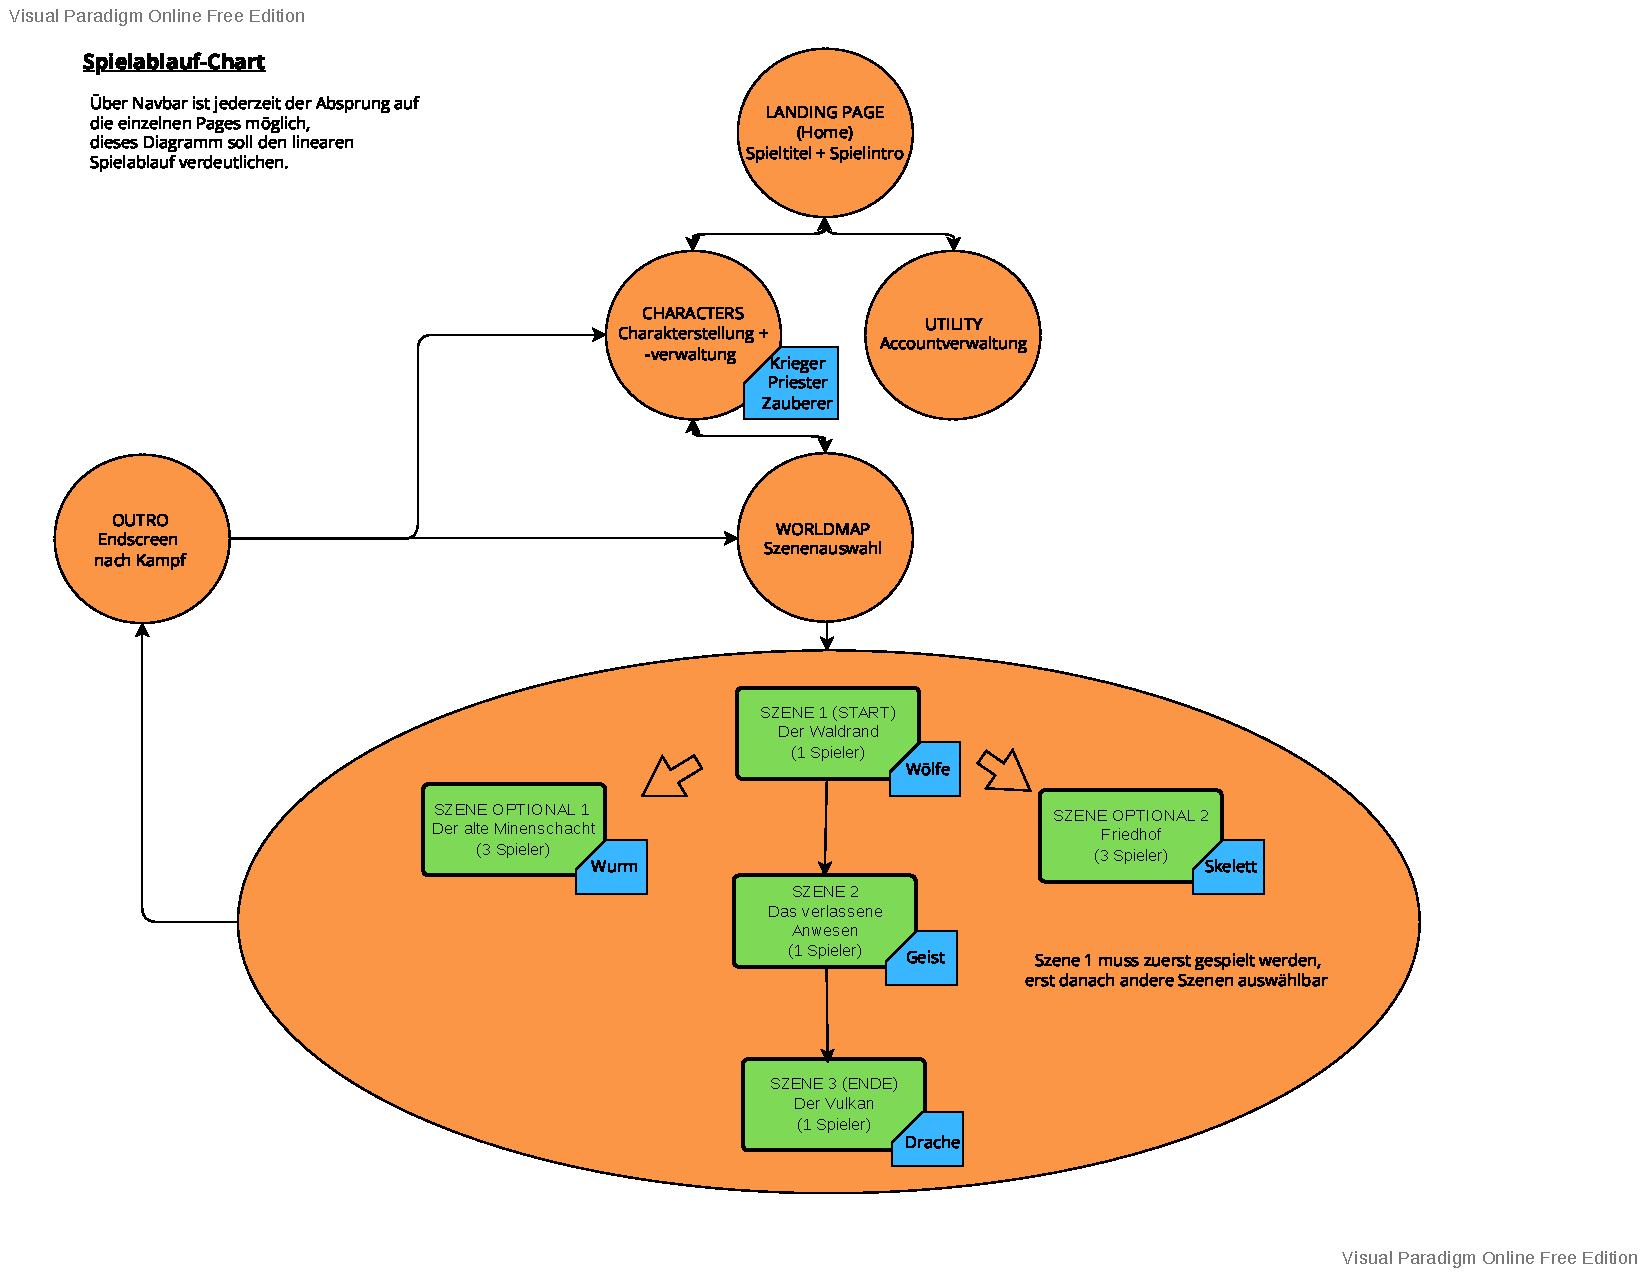
\includegraphics[width=1\textwidth, height=10cm]{2022-01-08-Spielablauf-Chart}
\end{figure}



\subsection{Infrastruktur und Code-Entwicklung}


\subsubsection{Infrastruktur}

Die für dieses Projekt eingesetzte Infrastruktur setzt auf verschiedene Komponenten, deren Zusammenspiel hier in einer vereinfachten Darstellung zu erkennen ist und im Folgenden näher beschrieben wird: 

\begin{figure}[H]
    \centering
    \label{fig:henning-dia-git-dev-server}
    \caption{Konzept: Entwicklung, Codeverteilung, Produktivnahme}
    \fbox{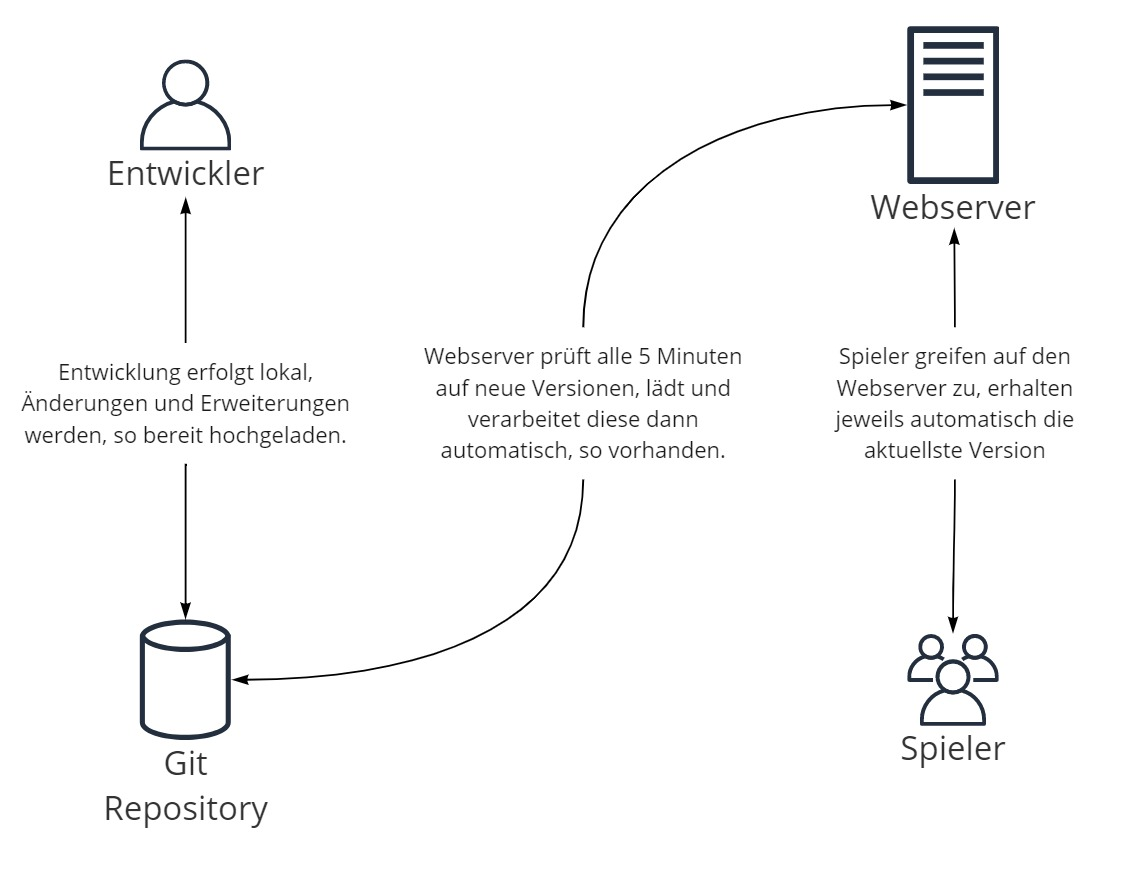
\includegraphics[width=0.8\textwidth]{henning-dia-git-dev-server}}
\end{figure}


Die Dienste selbst laufen auf einem für dieses Projekt bei der \textbf{HostEurope GmbH}\footnote{Siehe \url{https://www.hosteurope.de/Server/Virtual-Server/}.} angemieten, virtuellem Server. Das Produkt nennt sich \enquote{Virtual Server 10.0} und verfügt in der geringsten Austattung über 1 vCPU, 2 GB RAM sowie 40 GB SSD-Speicher. Auf dem Server läuft Debian 11. Der Server hat außerdem eine feste IP-Adresse. Einrichtungskosten gab es keine. Der Vertrag ist montalich kündbar. Der Mietpreis beträgt 5,99 EUR incl. MwSt. monatlich.

Weiter wurde bei \textbf{INWX GmbH}\footnote{Siehe \url{https://www.inwx.de/de/de-domain}.} zu dem Server auch eine Domain gekauft sowie entsprechende Namensservereinträge hinterlegt, die den Betrieb eines Traefik-Proxys mit Subdomains zu Domain erlauben. Auch hier gab es keine Einrichtungskosten. Der Preis für die Domain beträgt pro 5,97 EUR incl. MwSt. pro Jahr. 


Abseites der vorgenannten Hardware, stellt das gemeinsame \textbf{Git-Repository auf Github}\footnote{Siehe \url{https://github.com/tstsrv-de/rpg/}.} einen zentralen Punkt der Infrastruktur dar. In diesem Repository liegen alle Elemente des Projektes: Code, Skripte und Dokumentation.

Die Funktionen des Repositorys sind folgende: \begin{itemize}
    \item Entwickler übermitteln neue Inhalte in das Repository (push).
    \item Entwickler erhalten den stets aktuellen Entwicklungsstand aus dem Repository (pull, fetch).
    \item Der Server lädt neue Inhalte aus dem Repository automatisch und aktualisiert die Dienste.
    \item Alle Beteiligten und auch Dritte können über das Repository die Entwicklung nachvollziehen. 
\end{itemize}


Für den Update-Prozess des Servers und der Dienste wurde ein Cron-Skript erstellt, dass laufend prüft ob neue Commits im Repository vorhanden sind (siehe \textbf{Codelisting 1} unten, Zeile 5). Wenn ja, wird der Django-Webserver gestoppt (Zeile 7), die neuen Inhalte heruntergeladen, verarbeitet und der Django-Webserver im Anschluss wieder gestartet (Zeile 15). 

\textbf{Codelisting 1: \enquote{rpg/server-update-cron.sh}, gekürzt um Logging:}
\begin{lstlisting}[language=bash]
#!/bin/bash
cd /home/rjhadmin/tstsrv/
now=$(date "+%F %H:%M:%S")
git -C /home/rjhadmin/tstsrv/ fetch origin 
if  [ `git -C /home/rjhadmin/tstsrv/ rev-list HEAD...origin/main --count` != 0 ] 
then
    docker-compose --project-directory /home/rjhadmin/tstsrv/ stop rpg  
    git -C /home/rjhadmin/tstsrv/ reset --hard origin/main  
    git -C /home/rjhadmin/tstsrv/ fetch
    git -C /home/rjhadmin/tstsrv/ pull 
    chmod +x /home/rjhadmin/tstsrv/*.sh 
    docker-compose --project-directory /home/rjhadmin/tstsrv/ run rpg python rpg/manage.py makemigrations 
    docker-compose --project-directory /home/rjhadmin/tstsrv/ run rpg python rpg/manage.py migrate 
    docker-compose --project-directory /home/rjhadmin/tstsrv/ run rpg python rpg/manage.py loaddata db_sample_data.json 
    docker-compose --project-directory /home/rjhadmin/tstsrv/ start rpg 
\end{lstlisting}



Ein weiterer wesentlicher Punkt der Software-Infrastruktur ist \textbf{Docker sowie die Container} für den Django-Server, die Datenbank und den Reverse-Proxy. Hier stehen für die lokale Entwicklung \enquote{docker-compose}-Skripte für Windows und auch unixartige Systeme wie Linux und MacOS zur Verfügung. Ebenso für den Betrieb des Servers. Details zur Einrichtung und Nutzung wurden in der \textbf{Readme Repositorys}\footnote{Siehe \url{https://github.com/tstsrv-de/rpg/blob/main/README.md}.} hinterlegt. 


Der Traefik-Proxy wurde so eingerichtet, dass Anfragen auf den Ports HTTP 80 und HTTPS 443 angenommen werden. Anfragen an HTTP 80, werden automatisch umgeleitet an HTTPS 443. Die notwendigen Zertrifikate für die Subdomains werden vollautomatisch vom Traefik-Proxy über Letsencrypt angefordert und verwaltet. Als Grundlage für die Konfiguration diente eine Vorlage von Igor Bubelov\footnote{Siehe Github-Repository dazu \url{https://github.com/bubelov/traefik-letsencrypt-compose}.} die entsprechend um die Funktionen für den Django-Webserver und die Datenbank erweitert wurden.



Die hier entwickelte Konfiguration erweis sich als so verlässlich, dass auch ein anderes Projektteam (\textbf{Deskshare\footnote{Siehe \url{https://github.com/tstsrv-de/deskshare} bzw. \url{https://deskshare.tstsrv.de/}.}}) aus unserem Studiengang, ihre Dienste auf unserer Hardware unter einer eigenen Subdomian betreiben konnte. Die Anbindung an den Traefik-Proxy war möglich, auch die SSL-Zertrifikate wurden vollautomatisch erstelt. Weiter konnte auch des Update-Konzepts mittels Cron-Dienst und Github-Repository übernommen werden, so dass das andere Projektteam eigenständig entwickeln konnte. 


Die Ressourcen des Servers reichen hier für beide Projekte, auch in der Phase vor Abgabe der Arbeiten, aus: 

\begin{figure}[H]
    \centering
    \label{fig:henning-server-auslastung}
    \caption{Bildschirmfoto: Server Auslastung}
    \fbox{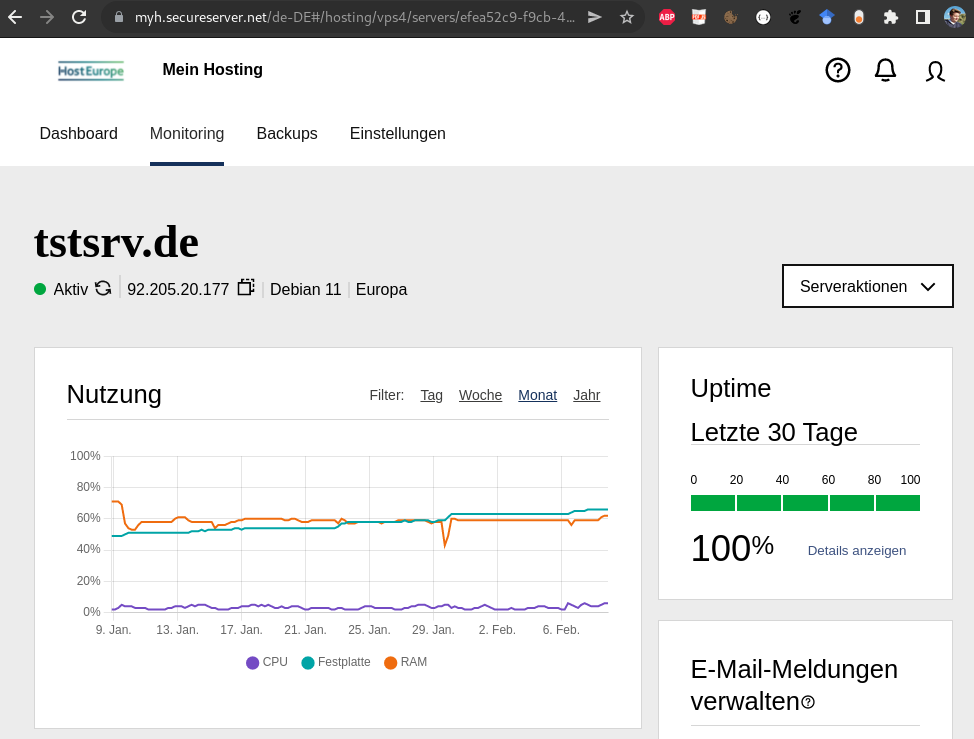
\includegraphics[width=0.8\textwidth]{server-auslastung.png}}
\end{figure}






\subsubsection{Initialisierung der Django-Anwendung}

Nach dem Aufbau der grundsätzlichen Funktionen des Servers (Update-Systemdienste und Cron-Skripte), wurde die Django-Anwendung initialisiert. Der Abaluf orientierte sich hier an den in den Vorlesungen gewonnenen Erkenntnissen und wurde im Anhang (siehe Anhang \ref{django-init}) stichpunktartig festgealten. 

Im Anschluss daran wurden dann zuerst grundlegende Funktionen für die Benutzer-Regeistrierung am System hinzugefügt. Das  insbesondere unter Nutzung von zwei Anleitungen\footnote{Siehe  \url{https://www.nintyzeros.com/2020/06/login-register-user\%20page-in\%20django.html} und \url{https://docs.djangoproject.com/en/3.2/topics/auth/default/\#built-in-auth-forms}.}.


Da das Projekt selbst die Entwicklung eines Spiels umfasste, wurde hier bewusst auf die Implementation von allen ansonsten mit einer Benutzerverwaltung im Zusammenhang stehenden Funktionen verzichtet. Es ist somit \textbf{nicht möglich}, seinen Benutzer z.B. zu löschen oder \textbf{ein vergessenes Passwort} zu erneuern. Unser Fokus lag hier, den Anforderungen entsprechend, auf der Entwicklung der Hauptanwendung. 

Es wird hier in dieser Dokumentation auch nicht weiter auf die implementierte Benutzerverwaltung eingegangen, da es sich um weithin bekannte Standart-Features von Django handelt.

Mit Abschluss der Einrichtung der Django-Anwendung, liegt ein mit den bekannten Funktionen (wie Datenbankmodelle, Benutzerverwaltung, DB-Migrationen, ...) nutzbarer Django-Webserver vor. 
Für die Entwickler und die Entwicklung selbst, ist die direkte Interaktion mit dem Django-Webserver selbst, nicht mehr notwendig. Die entwickelten Skripe, starten den Webserver mit allen notwendigen Paramentern selsbtständig und führen vorher auch notwendige Schritte wie \enquote{makemigrations, migrate oder loaddata} selsbtständig aus. Beispielhaft hier ein Auszug aus dem Skript für den Start der lokalen Entwicklungsumgebung unter unixartigen Betriebssystemen\footnote{Siehe \url{https://github.com/tstsrv-de/rpg/blob/main/local-dev-start.sh}.}: 

\begin{lstlisting}[language=bash]
#!/bin/bash
docker-compose -f local-dev-docker-compose.yml up -d
docker-compose -f local-dev-docker-compose.yml exec rpg python rpg/manage.py makemigrations
docker-compose -f local-dev-docker-compose.yml exec rpg python rpg/manage.py migrate
docker-compose -f local-dev-docker-compose.yml exec rpg python rpg/manage.py loaddata db_sample_data.json
docker-compose -f local-dev-docker-compose.yml stop
docker-compose -f local-dev-docker-compose.yml up 
\end{lstlisting}


\subsubsection{Datenbankmodell}

Aus den ersten Gesprächen und Austausch zum Projekt und den später formulierten Anforderungen wurden Erste Konzepte und Ideen zu Papier gebracht. Dabei wurden auch erste Zeichnungen zu einem möglichen Datenbankmodell erstellt. In bzw. zu den späteren Projektbesprechungen wurden konkretere Zeichnungen erstellt. 

\begin{figure}[H]
    \centering
    \label{fig:henning-entwurf-datenbankmodell}
    \caption{Datenbankmodell Entwurfsprozess}
    \subfloat[Entwurfszeichnung vom 23.11.2021]{\fbox{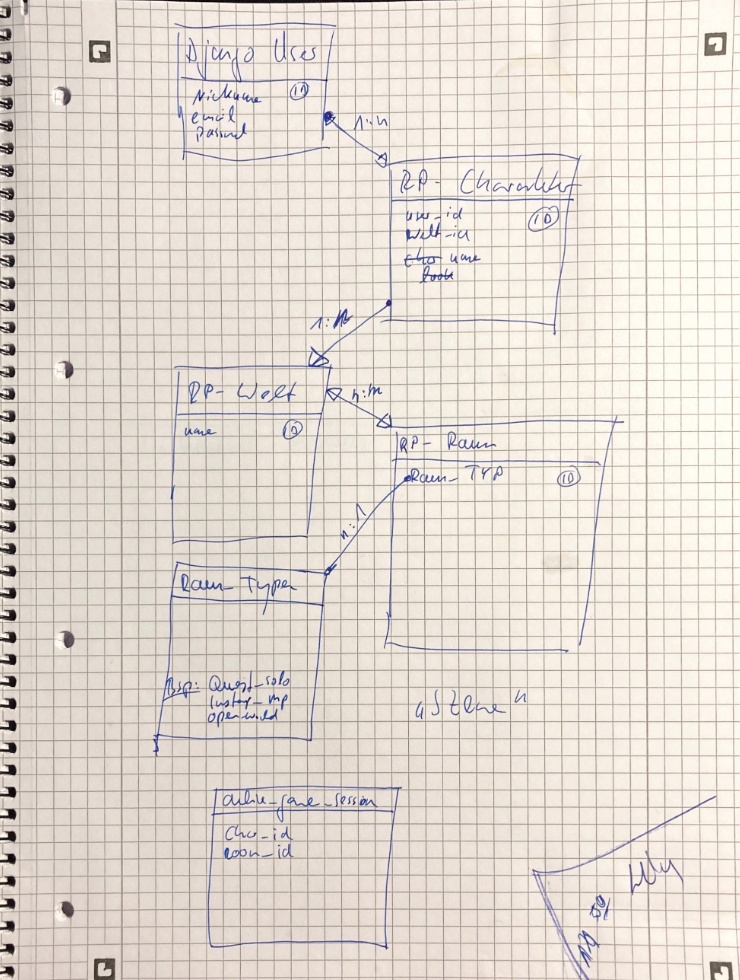
\includegraphics[width=0.5\linewidth]{2021-11-23-erstes-db-konzept}}}
    \subfloat[Weiterentwickelter Entwurf (05.12.2021)]{\fbox{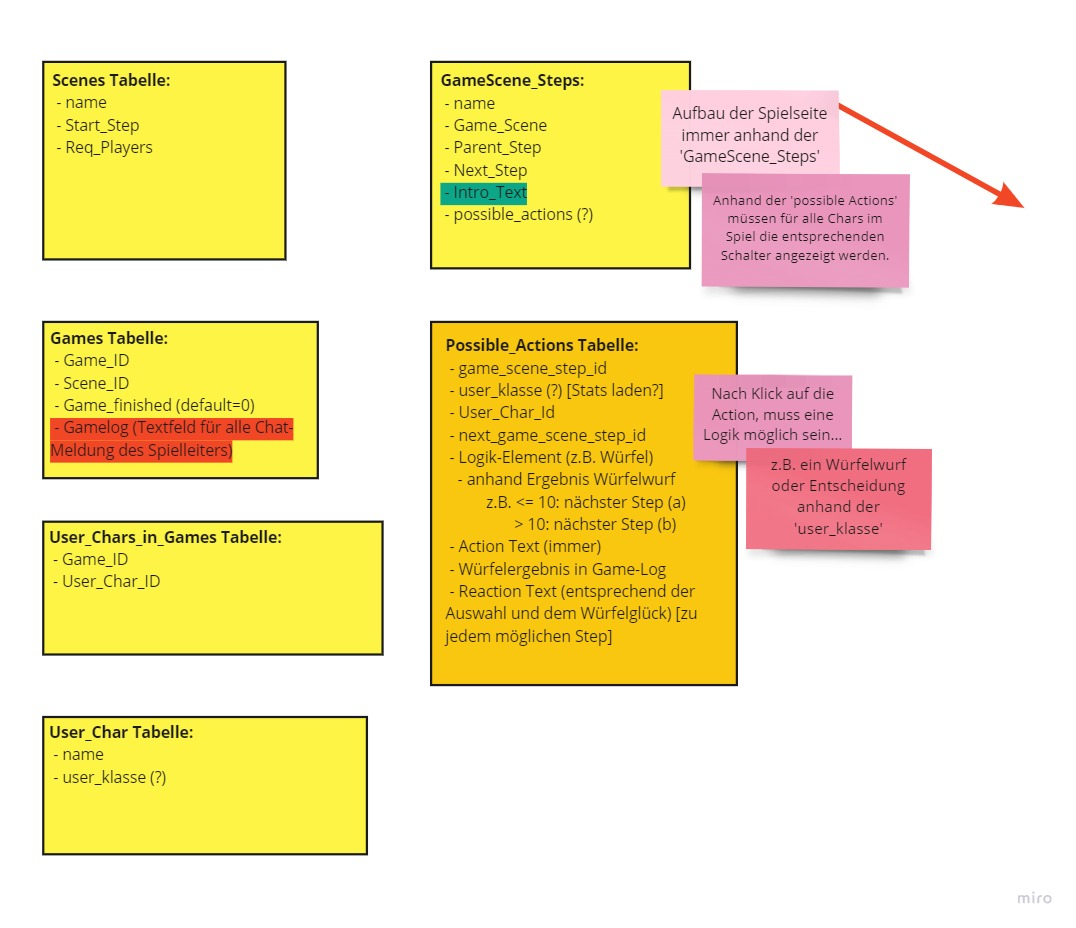
\includegraphics[width=0.5\linewidth]{2021-12-05-Projketbesprechung-Miro-c}}}
\end{figure}

Fortsetzung auf der Folgeseite. 

\newpage

Hier eine Darstellung des Datenbankmodells als Diagramm sowie anschließend die ausführliche Beschreibung jeweils mit Stand vom 10.02.2022. 

\begin{figure}[H]
    \centering
    \label{fig:henning-datenbankmodell-final}
    \caption{Datenbankmodell final (Stand 10.02.2022)}
    \fbox{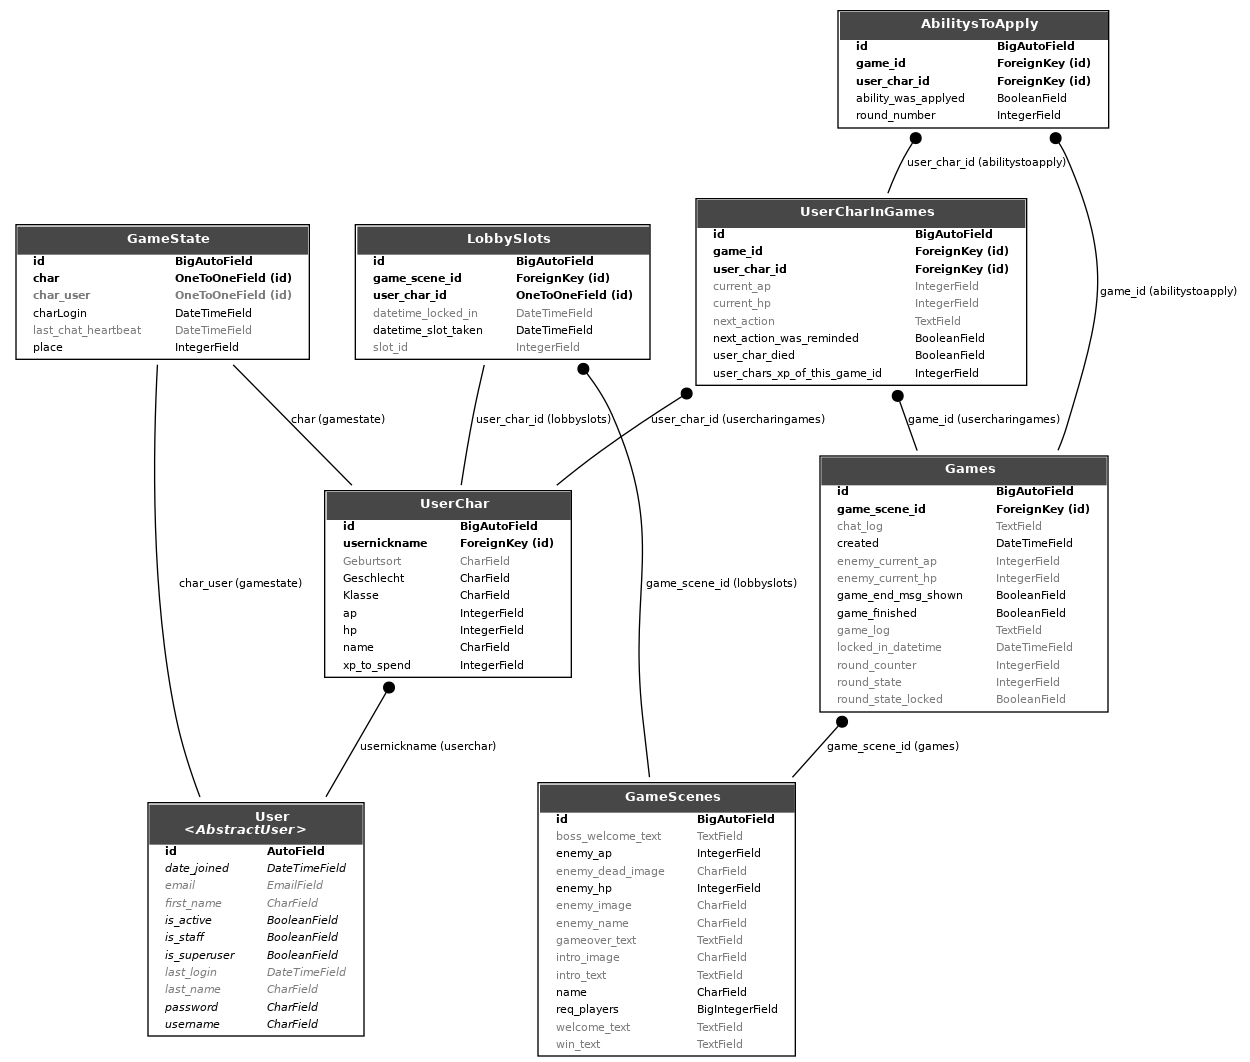
\includegraphics[width=0.8\textwidth]{db-modell-final.png}}
\end{figure}


Der Aufbau der des Datenbankmodells beginnt logisch mit der \textbf{Benutzertablle} sowie den anderen, von Django systemseitig erstellten Tabellen, auf die hier nicht weiter eingegangen wird.

Auf die Benutzertabelle setzt eine \textbf{Tabelle für Charaktere} (\textit{UserChar}) auf. Darin enthalten und jeweils einem Benutzer zugeordnet, sind alle Daten zu den Spielercharakteren. Neben dem Namen und der Klasse sind in der Tabelle auch veränderliche Attribute wie die Angriffspunkte und Lebenspunkte sowie noch zu verteilende Erfahrungspunkte abgespeichert. 

Bei der Erstellung eines neuen Charakters werden die Start- bzw. Standartwerte für Lebens- und Angriffspunkte aus einer besonderen \textbf{Konfigurationstabelle} (\textit{myrpgconfig}) abgerufen und für die Erstellung des neuen Charakters entsprechend der ausgewählten Klasse, abgespeichert. In dieser Konfigurationstabelle wurden weiter auch für \textbf{alle Konstanten} die im Laufe der Entwicklung Einzug in den Programmcode gehalten haben, in einem späteren Schritt in diese Tabelle transportiert. Dies umfasst tatsächlich komplett alle Konstanten. Beispielhaft genannt seien hier z.B. der Faktor für die Berechnung von Erfahrungspunkten aus dem verursachten Schaden, der Minimal- und Maximalfaktor bei der Berechnung des bei einem Angriff entstandenen Schaden aus den Angriffspunkten heraus sowie auch die Laufzeiten in Rundenzahl sowie die Stärke der Fähigkeiten der einzelnen Klassen. 

Das erlaubt es, die gesamte Konfiguration des Projektes und ebenso auch das Balancing über die Administrationsoberfläche von Django unkompliziert zu verändern und zu pflegen. Die Konfigurationstabelle umfasst 21 Einstellungen. Zu jeder Einstellung sind in der Datenbank selbst auch entsprechende Erklärungen zur genauen Verwendung und Nutzung hinterlegt. Auch ist es möglich \textbf{verschiedene Datentypen in der Konfigurationstabelle} abzuspeichern und abzurufen. Folgende Hilfsfunktion wurde dazu in der Datei \enquote{rpg\_tools.py}\footnote{Siehe \url{https://github.com/tstsrv-de/rpg/blob/main/rpg/rjh_rpg/rpg_tools.py\#L63-L80}.} erstellt: 

\begin{lstlisting}[language=python]
def rpg_get_config(config_to_get):

    try: 
        config_type = MyRpgConfig.objects.get(name=config_to_get).type
    
        if config_type == "int":
            return int(MyRpgConfig.objects.get(name=config_to_get).value)

        elif config_type == "str":
            return str(MyRpgConfig.objects.get(name=config_to_get).value)

        elif config_type == "float":
            return float(MyRpgConfig.objects.get(name=config_to_get).value)
    
    (...)
\end{lstlisting}


Neben der Benutzertabelle, Charatertabelle und der Konfigurationstabelle gibt es eine ganze Menge an Tabellen für das Spiel selbst. Zentral ist dabei die \textbf{Grundtabelle der Level} (\textit{GameScenes}): Diese ist als Bauplan der Level zu verstehen. Enthalten sind alle notwendigen Informationen um ein neues Spiel in einem der Level starten zu können: Der Name des Gegeners, die Texte und Werte des Gegners. Aber auch die Anzahl der für diesen Level notwendigen Spieler. Ebenso sind alle Texte zum Level (Intro, Gewinn- und Gameover-Nachricht, ...) darin enthalten. 

In der \textbf{Hilfstabelle für den Spieler-Staus} (\textit{GameState}) wird jeweils der aktuelle Standort eines Spielers hinterlegt. Mit Standort ist dabei die aktuell aufgerufene Seite des Spieles gemeint. Es kann darüber nachvollzogen werden ob der Spieler sich gerade auf der Weltkarte befindet oder in einer der Level-Lobbys. Auch wird darin ein Zeitpunkt des letzten Datenpaketes aus dem Chat hinterlegt. Darüber ist es möglich, Spieler nach Ablauf einer gewissen Zeit (Sekunden), automatisch aus dem Chat zu entfernen. 

Innerhalb der Level-Lobby können über die \textbf{Hilfstabelle für die Level-Lobbys} (\textit{LobbySlots}) die bereits belegten Plätze für ein Spiel nachgehalten werden. Die Spieler belegen in der Lobby mit einem Klick einen verfügbaren Platz. Sind dann alle Plätze des Levels belegt, wird nach Ablauf eines Countdowns \textbf{ein neues Spiel gestartet}.

Mit Spielstart wird in der \textbf{Spieltabelle} (\textit{Games}) ein neues Spiel angelegt. Dieses Spiel darin trägt eine Verknüpfung zum Bauplan (Grundtabelle der Level: \textit{GameScenes}), ein Game-Log in dem alle Texte des Spiels gespeichert werden, die aktuellen Lebens- und Angriffspunkte des Gegeners sowie auch alle \textbf{Informationen zum Rundenstatus} des Spiels.

Gleichzeitig mit der Anlage des Spiels selbst, werden in der \textbf{Hilfstabelle für die Spieler- und Spiel-Zurodnung} (\textit{UserCharInGames}) für jeden für das Spiel angemeldeten Spieler ein entsprechender Eintrag erzeugt. Während des Spiels werden darin alle Werte des Spieler hinterlegt. Auch ob der Spieler in diesem Spiel bereits verstorben ist, wird darin gespeichert. 

Letzte mit dem Spielablauf im Zusammenhang stehende Tabelle ist eine \textbf{Spezialtabelle für die aktivierten Fähigkeiten der Spieler} (\textit{AbilitysToApply}). Darin wird immer wenn in einem Spiel ein Spieler seine Fähigkeit aktiviert, alle Informationen abgespeichert die für die spätere Wirksamkeit notwendig sind. Entscheidet sich z.B. der Priester in Runde 3 seine Fähigkeit anzuwenden (und wirkt diese über 4 Runden), werden in der Tablle entsprechende Einträge für Runde 4, 5, 6 und 7 mit Bezug auf den Priester und die Heilung hinterlegt. Wendet die Runden- bzw. Spiellogik diese Fähigkeit an, wird ein entsprechndes Kennzeichen dazu in dem Datensatz gesetzt (\textit{ability\_was\_applyed = true}).





\subsubsection{Code-Entwicklung}

In der Zeit vom 25.11.2021 bis zum 09.01.2022 wurden von Henning Beier im weiteren das Backend, das Datenbankmodell und die wesentlichen Funktionen des Spiels, entsprechend der in den Projektbesprechungen festgehaltenen Anforderungen, entwickelt.



\textbf{Entwicklung, Mittwoch 24.11.2021}

Einbau von Grundlagen: 
\begin{itemize}
    \item Update der Django-Basis Installtion bzw. des Projektes (Commit \url{https://git.io/JSqbt}). 
    \item Auto-Download und restart der Docker-Container bei neuen Commits im Repository auf Github per Cron-Jobjob-Script (siehe \url{https://git.io/JStjW}).
\end{itemize}


\textbf{Entwicklung, Donnerstag 25.11.2021}

Einbau der Charaktere als Datenbank-Modell und View in Django (Commit \url{https://git.io/JSmOd}).



\textbf{Entwicklung, Samstag 27.11.2021}

Einbau der Weltkarte bzw. Levelauswahl (Commit \url{https://git.io/JSmG8}).



\textbf{Entwicklung, Sonntag 28.11.2021}

\begin{itemize}
    \item Einbau einer Web-Sockets Chat-Funktion unter Nutzung einer Anleitung\footnote{Siehe \url{https://github.com/veryacademy/YT-Django-Project-Chatroom-Getting-Started}. } (Commit \url{https://git.io/JSmlS} sowie folgender Commits von diesem Tag).
    \item (Teilweise) Installation der Entwicklungsumgebung, Docker sowie Git bei Julian und Rico sowie jeweils zwei erste Test-Commits incl. anschließendem Auto-Update des Servers (Rico: \url{https://git.io/JSmKV} und Julian: \url{https://git.io/JSmoF}).
\end{itemize}



\textbf{Entwicklung, Montag 29.11.2021}

Erstellung eines Web-Sockets für eine Counter-Funktion incl. der notwendigen Anpassungen an Datenbankmodell, der Django-Reciver und -Consumer (Commit \url{https://git.io/JSmDa}).



\textbf{Entwicklung, Dienstag 30.11.2021}

Einbau einer Lobby und einer Chatfunktion in dieser Lobby -- Jeweils abhängig von der Lobby werden dynamisch Websockets geöffnet (Commits \url{https://git.io/JSm5n} und \url{https://git.io/JSm5N} sowie weitere Anpassungen und Korrekturen in den Commits vom 01.12.2021).


\textbf{Entwicklung, Samstag 04.12.2021}

Flask8 als Code-Linter genutzt und einige Anpassungen entsprechend vorgenommen (Commit \url{https://git.io/JSmN2}).


\textbf{Entwicklung, Sonntag 05.12.2021}

Einbau der Spielseite selbst als logischer Schritte nach der Weltkarte (als Levelauswahl) und der Lobby (Spielfindung /-erstellung) (Commits \url{https://git.io/JSYLS}, \url{https://git.io/JSYqd} und \url{https://git.io/JSYmV}).



\textbf{Entwicklung, Sonntag 12.12.2021:}

Als Grundlage der Dokumentation eine an APA-Zietierrichtlinien angepasste Variante der LaTeX-FOM-Vorlage\footnote{Siehe \url{https://github.com/andygrunwald/FOM-LaTeX-Template}.} in der Git-Repository eingefüht und für das Projekt hier angepasst. Dort erfolgt nun laufen auch die Dokumentation (Commit \url{https://git.io/JSYOZ}). 



\textbf{Entwicklung, Sonntag 19.12.2021:}

An diesem Tag wurden weitere, notwenige Grundlagen für die Integration der Spiellogik eingebaut. Das insbesondere in Vorbereitung auf die kommenden Anpassungen und Entwicklungen die in der Projektbesprechung vom 11.12.2021 besprochen wurden. 
Konkret: 

\begin{itemize}
	\item Prüfung auf den Seiten Chars, Worldmap und Lobby ob dieser Benutzer ein aktives Spiel hat. Falls ja, wird der Benutzer auf diese Seite umgeleitet.
	\item Grundfunktion für das Beenden von einem Spiel eingebaut: Man kann nun per Klick im Spiel, das Spiel beenden.
	\item Daran anschließend eine Prüfung im laufendem Spiel, ob das Spiele beendet wurde und falls ja, Anzeige eines Endbildschirms.
\end{itemize}

Die Entwicklung der Grundlagen an diesem Tag wurde mit Fokus auf Modularisierung erledigt. Der Code der jeweiligen Funktionen wurde in einzelnen Dateien ausgelagert um Wiederverwendbarkeit und Lesbarkeit zu erhöhen. 

Die zugehörigen Commits sind insbesondere: 
\url{https://git.io/JDjKl} und 
\url{https://git.io/JDjKB}


\textbf{Entwicklung, Dienstag 21.12.2021:}

Grundlagen des Kampfsystems entsprechend der Projekt-Besprechung vom 11.12.2021 (Abbildung \ref{fig:2021-12-11-Projekt-Besprechung}) sollen implementiert werden.

Vorbereitungen: 

\begin{itemize}
    \item Tabelle "GamesScenesSteps" und Verknüpfungen entfernen (Commits \url{https://git.io/JDjKz} und \url{https://git.io/JDjKg})
    \item Kampf-/Gamelog erzeugen: Darin werden alle Meldungen aus dem Spiel wie z.B. Kampftexte, Schaden, Aktionen, Systemmeldungen und alles andere denkbare angezeigt und gespeichert. Getrennt davon soll der Chat-Log dargestellt werden. Dazu werden in der Tabelle "Games" zwei neue Textfelder erzeugt (Commit \url{https://git.io/JDj63}). 
    \item Anzeige des Game-Logs auf der Spielseite. Schreiben von Nachrichten in das Gamelog als ersten Test des grundlegend umgestellten Seitenaufbaus: Es werden nur noch einzelene Elementinhalte per Websocket transportiert, nicht mehr ganze HTML-Code-Blöcke (Commit \url{https://git.io/JyeJQ}).
\end{itemize}


\textbf{Entwicklung, Montag 27.12.2021:} \label{ref-runden-impl}

Weitere Entwicklungen entsprechend der Projekt-Besprechung vom 11.12.2021 (Abbildung \ref{fig:2021-12-11-Projekt-Besprechung}):

\begin{itemize}
    \item Eintrag ins Gamelog zum Spielstart (Commit \url{https://git.io/JyBRf}).
    \item Rundensystem implementieren. Dazu mindestens notwendig: Lebens- und Angriffspunkte der User-Chars sowie des Gegners. 
    \begin{enumerate}
        \item Erster Schritt: Definition des Ablaufes einer Runde als Pseudo-Code: 
            \begin{enumerate}
                \item Gameloop-Schleife: [round-state]
                \item Aktion von Gegner ausführen (Schaden) [100]
                \item Prüfen ob User-Char tod ist (HP < 1 = Dead-Flag: True) [200]
                \item Prüfen wie viele User-Chars noch leben (n < 1 = Gameover-Flag: True, break-Gameloop-Schleife) [300]
                \item Aktionen der User-Chars aufnehmen (Entscheidung für nächste Aktion von jedem Spieler annehmen + wegspeichern) [400]
                \item Alle Aktionen der User-Chars ausführen (Aktionen laden und ausführen: Schaden, Aktion, Passen) [500]
                \item Nach jedem Spieler, prüfen ob Gegner besiegt wurde (HP < 1 = Win-Flag: True, break-Gameloop-Schleife) [immernoch 500]
                \item Rundencounter +1 [600]
                \item Gameloop-Schleife nächster Durchlauf [700, zurück zu 100]...
            \end{enumerate}
    Steuerung über "round-state" Hilfsvariable, gespeichert in Games-Tabelle (Default=0, Gameover=990, Win=995). Da der Aufruf der Spiele-Logik über den Websocket-Heartbeat der Spieler erfolgt, müssen die Arbeitsschritte sehr kleinteilig sein und diese laufend in kleinen (kleinsten?) Schritten weggepeichert werden. Möglicherweise ergibt sich ein Sync-Problem (Commit \url{https://git.io/JyRml})
    \item Zweiter Schritt: HP und AP bei User-Chars implementieren, damit AP aus "round-state 100: Gegner führt Schaden aus" durchgeführt werden kann (Commit \url{https://git.io/JyRWD}).  
    \end{enumerate}
\end{itemize}


\textbf{Entwicklung, Dienstag 28.12.2021:}

Fortführung der Entwicklungen vom Vortag. Hier insbesondere nun die Implementation der aller Funktionen der Runden- bzw. Spiellogik:

\begin{itemize}
    \item Auswahl eines zufälligen, lebenden Spielercharakters und zufügen von Schaden durch den Gegener. Außerdem Erweiterung Runden-/Gameloop und Fortschreiben des Game-Logs (Commit \url{https://git.io/JygDz}).
    \item Nächster Rundenschritt 200: Prüfen ob Spieler gestorben sind und Meldung im Game-Log ausgeben falls in aktueller Runde gestorben (Commit \url{https://git.io/Jya3H}). 
\end{itemize}


\textbf{Entwicklung, Mittwoch 29.12.2021:}

Weitere Implementation von Rundenlogik:

\begin{itemize}
    \item Rundenschritt 300: Feststellen ob alle Spieler verstorben sind, falls ja in Spielende springen (Commit \url{https://git.io/Jy1Lu}).
    \item Tests ergaben Probleme beim Spiel mit mehreren Spielern. Die Rundenlogik wird dann gleichzeitig vorangetrieben. Dadurch werden manche Aktionen und Rundenschritte mehrfach ausgeführt. Ein Versuch das Problem mit einem Token (ähnlich einem Semaphor) zu lösen, brachte leider noch keinen abschließenden Erfolg. Der Singleplayer aber, geht fehlerfrei. Das Problem wird daher zurückgestellt und nun zuerst die Entwicklung weiterer Punkte fortgeführt (Commit \url{https://git.io/Jy1qZ}).
    \item Als Workaround für oben genanntes Problem im Mulitplayer wurde nun eingestellt, dass immer nur der erste Spieler eines Spiels die Rundenlogik vorantreibt. Das ist etwas mehr fehleranfällig als eine korrekte Tokenlösung, wird für das Projekt hier aber vorerst ausreichend sein (Commit \url{https://git.io/Jy1su}).
    \item Umfangreiche Erweiterungen und Anpassungen für das Anzeigen der User-Chars auf der Spieleseite, darstellen und aussteuern der Aktions-Buttons, das einsammeln der Aktionen in der Datenbank und ebenso bereits das zurücksetzen beim Rundenwechsel (Commit \url{https://git.io/JyDlp}).

    \begin{figure}[H]
        \centering
        \caption{29.12.2021: Bildschirmfoto zum Entwicklungsstand mit Runden-Status 400.}
        \label{fig:2021-12-29-Bildschirmfoto-Entwicklungsstand-Runden-Status-400.png}
        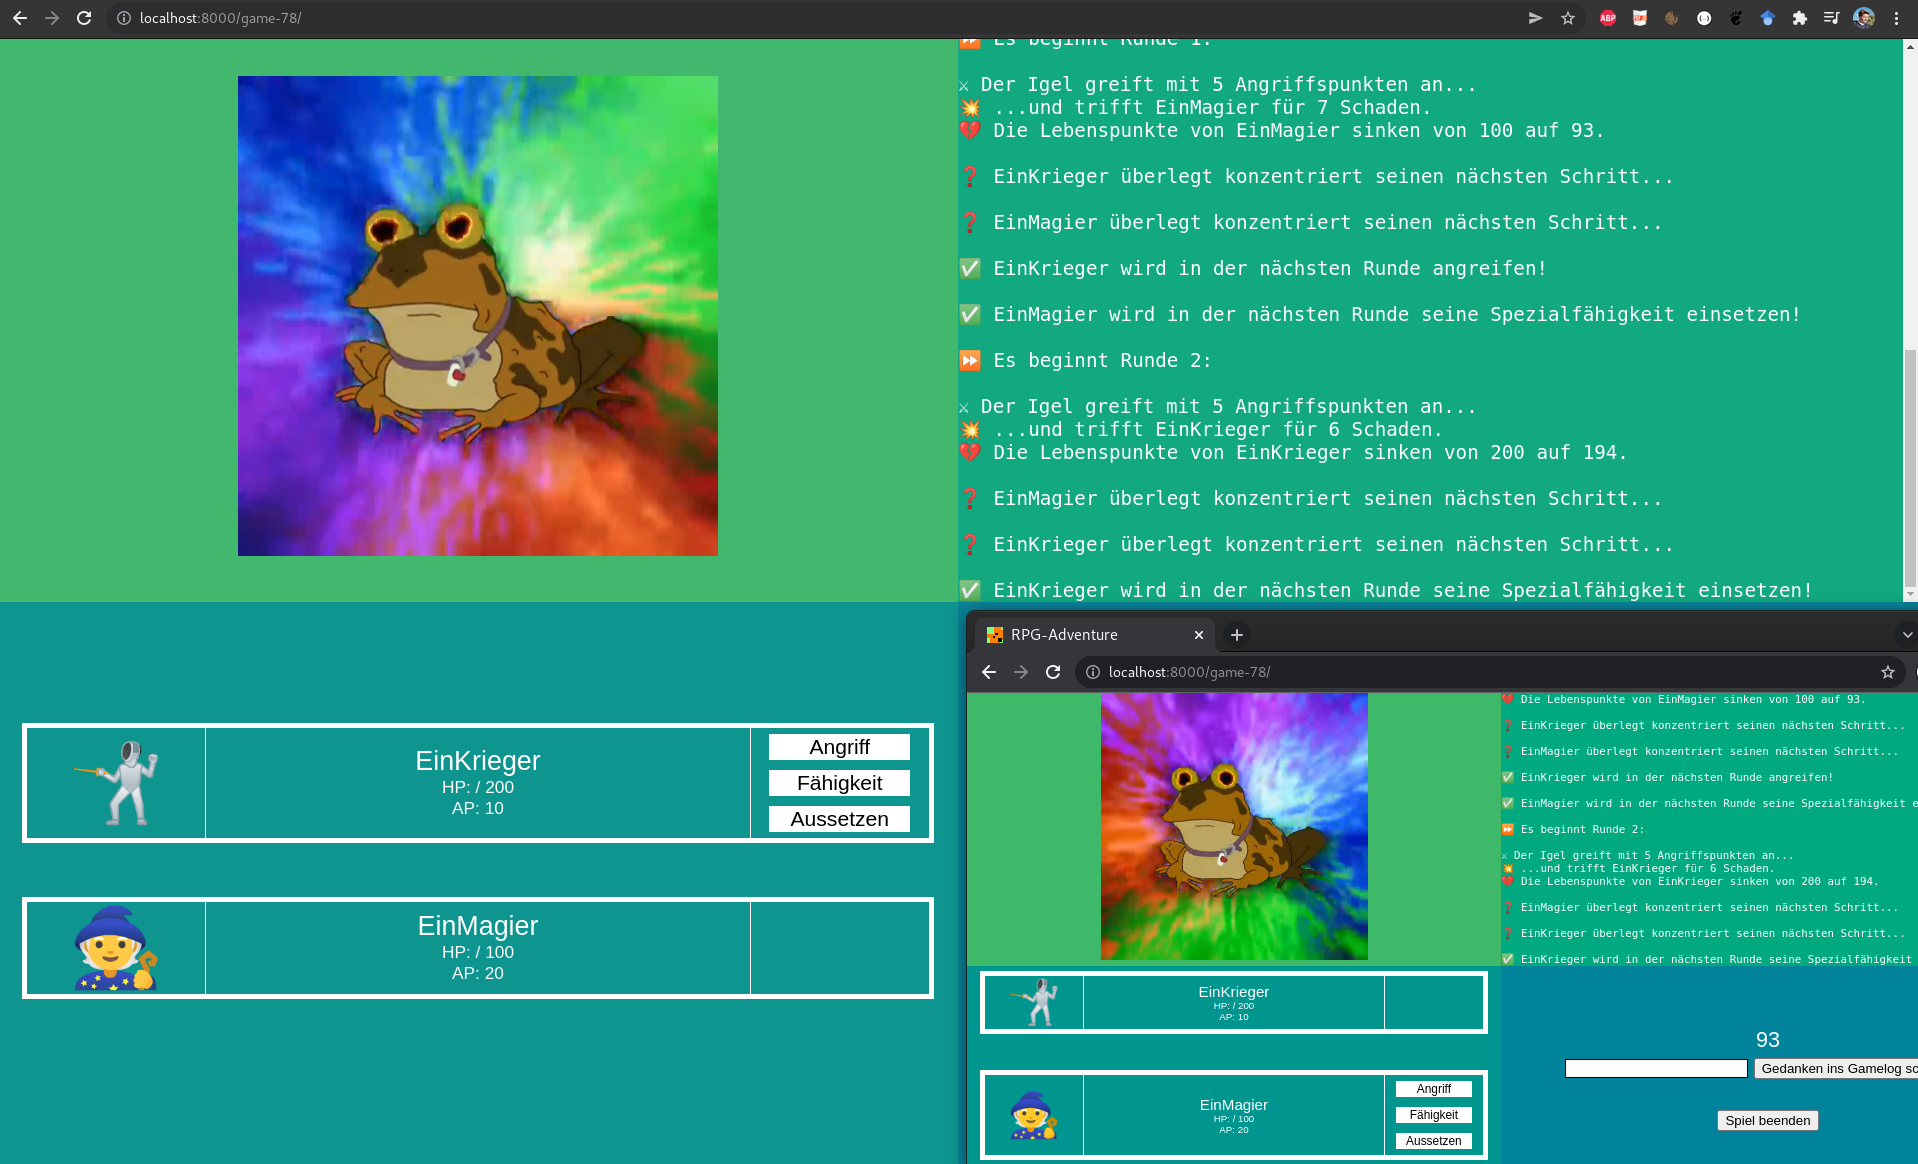
\includegraphics[width=0.7\textwidth]{2021-12-29-Bildschirmfoto-Entwicklungsstand-Runden-Status-400.png}
    \end{figure}

    \item Die Chatfunktion wurde implementiert. Hier jedoch abweichend vom Plan direkt als Meldungen im Game-Log und nicht in einem gesonderten Chat-Log und Chat-Fenster. Julian war damit im kurzen Teams-Gespräch gestern einverstanden. Den Aufbau der Game-Seite entsprechend angepasst und dem Game-Log deutlich mehr Raum eingeräumt. Außerdem weitere Anpassungen am Design und Style (Commit \url{https://git.io/JyDRK}).

\end{itemize}


\textbf{Entwicklung, Donnerstag 30.12.2021:}

Abschließender Schritt in der Implementation der Rundenlogik:

\begin{itemize}
    \item Die Schadensfunktion für Spieler wurde eingebaut: Damit kann dem Gegner nun Schaden zugefügt werden. Außerdem Prüfung auf Tod des Gegners incl. entsprechender Medlung (Commit \url{https://git.io/Jy9E7}).
\end{itemize}

Offen sind nun als nächste Schritte noch:
\begin{enumerate}
    \item Fähigkeiten der Spieler in Rundenlogik implementieren.
    \item Abschlussbildschirm für Sieg und Gameover konzeptionieren und implementieren. 
    \item Charakterentwicklung bei Sieg implementieren.
    \item Erweiterung der Infrastruktur aus Scripten, Anleitungen und des Git-Repos hin zum laden eines Default-Datensatzes (JSON-Datei) mit nutzbaren Spieldaten (insbesondere für Testzwecke und Nutzungen durch Dritte).
\end{enumerate}


\textbf{Entwicklung, Freitag 31.12.2021:}

Abarbeiten der zuletzt genannten, nächsten Schirtte. Hier: 

\begin{itemize}
    \item Die Charakterentwicklung wird mit Erfahrungspunkten gelöst: Durch Aktionen im Spiel bzw. Kampf (Schaden bekmmen, Schaden austeilen, Fähigkeiten nutzen) bekommen die entsprechenden Charaktere sofort entsprechende Erfahrungspunkte gutgeschrieben. Wird das Spiel gewonnen, werden alle von allen teilnehmenden Spielern in dieser Runde erspielten Erfarungspunkte noch einmal verdoppelt und jedem der Spieler gutgeschrieben. Verwendet werden können diese Erfahrungspunkte dann in der Charakteransicht um damit z.B. Lebenspunkte (HP) oder Angriffspunkte (AP) zu erhöhen (Commit \url{https://git.io/Jy7gl}).
\end{itemize}


\textbf{Entwicklung, Samstag 01.01.2022:}

Nach kurzer Abstimmung und Vorstellung meiner Ergebnisse bei Julian, letzte Anpassungen bzw. Entwicklungen: 

\begin{itemize}
    \item Ausgabe der erhaltenen XP beschleunigt: Es werden nun immer 10\% (aufgrundet auf die nächste Ganzzahl) der XP ausgegeben (Commit \url{https://git.io/JSTIq}).
    \item Einbau der Charakter-Fähigkeiten (Commit \url{https://git.io/JSkKJ}):
    \begin{itemize}
        \item Priester: Gruppe heilen=Alle HP erhöhen
        \item Zauberer: Schaden der Gruppe erhöhen=Alle AP erhöhen
        \item Krieger: Gegner blocken=AP Gegner verringern
    \end{itemize} 
    Damit die Fähigkeiten über mehrere Runden wirken können, musste eine Hilfstabelle angelegt werden: "AbilitysToApply". Hieraus werden zum Rundenwechsel die jeweils anzuwendenden Fähigkeiten gelesen und auf die relevaten Zahlen gewirkt. 
    \item Beispieldaten hinzugefügt und automatisches laden in die Datenbank über die local/dev-Skripte eingefügt (Commit \url{https://github.com/tstsrv-de/rpg/commit/1bfa99e89ddf2dbe817bdee2c870d1ddbe4f23c1}).
\end{itemize} 


\textbf{Entwicklung, Sonntag 02.01.2022}

Ein kurzer Anwendungstest mit einem versierten RPG-Spieler und IT-affinen Nutzer. Notizen dazu: 

\begin{itemize}
    \item Hinweis beim betreten der Lobby, dass das Spiel erst startet, wenn man einen "Platz-belegt" hat: Sofort erledigt!. 
    \item Man versuchte die Interaktion mit dem Spiel per Textkommandos über die Chatzeiel. Ineteresannte Alternative zur Nutzng der Buttons: Üübertragen in Ausblick(\ref{ausblick}). 
    \item Der erste Level ist mit über 10 Runden deutlich zu lang und muss verkürzt werden: Sofort erledigt!
\end{itemize}

Weiter wurden alle im Code enthaltenen Variablen und Konstanten in die Datenbank ausgelagtert. Dazu wurde eine neue Tabelle "MyRpgConfig" angelegt, alle Werte dorthin transportiert und im Code enstprechende Abfragen sowie weitergehende Anpassungen (z.B. Schleifen x-Fach durchlaufen) vorgenommen. Auch wurden die Beispiel- bzw. nun Basisdaten für die Datenbank entsprechend erweitert (Commits \url{https://git.io/JSGJD} und \url{https://git.io/JSGJ7}).


\textbf{Entwicklung, Sonntag 09.01.2022}

Nach letzter Projektbesprechung\ref{fig:2022-01-06-Projektbesprechung} in der vorallem Deatils zum weitern Ablauf, Meiliensteinen und zeitlichen Fristen besprochen wurden, kommen nun erste konkrete Texte zum Spiel-Inhalt. Dazu wurde das Spiel erweitert: Der bisherige Introtext ergänzt um eine Begrüßung durch den Gegener, sowie 2 Varianten (Gameover und Win) zum Spielende (Commit \url{}).


\newpage


\subsection{Vorstellung des Ergebnisses Rico}


\subsection{Spieldesign} Am Anfang der Entwicklung musste ein geeignettes Setting für das geplante RPG* gefunden werden. Zur Auswahl standen die beiden klassischen, den meisten bekannten Arten von Spieleuniversen zur Auswahl. Das eine wäre futuristisches Scifi und das andere eher mittelalterliches Fantasy. 

In der Frühen Phase der Entwicklung war beim Spieldesign ursprünglich geplant ein RPG zu entwickeln, dass viele Elemente vom klassischen Pen and Paper Rollenspielen*, wie z.B. Dungeons and Dragons enthält. Man wollte unterschiedliche Charakterklassen, die sich in ihrer Ausrüstung, wie individuelle Waffen und Rüstungen, sowie ihren speziefischen Fähigkeiten klar von einander unterscheiden. Ein Levelsystem, bei dem die einzelnen Charaktere von Abenteuer zu Abenteuer ihre Fähigkeiten verbessern und bessere Ausrüstung in Form von Beutegut finden können, sollte auch enthalten sein. Das Entwicklerteam hat sich dann für das Fantasysetting entschieden, weil man der Ansicht war, dass sich die vorher genannten Eigenschaften damit besser umsetzen lassen würden. Speziel die unterschiedlichen Eigenschaften der Charakterklassen waren bei dieser Entscheidung massgeblich, denn eine Eingrenzung auf die besonderen Fähigkeiten der unterschiedlichen Spielfiguren, wie z. B. einen Tank*, einen Heiler* und einen Damagedealer*, schien im Scifi-Hintergrund nicht so einfach und für den Spieler nicht schlüssig zugestalten.

Die Überlegungen führten somit schon am Anfang recht schnell zu den bereits erwänten unterscheidlichen Spielfiguren, die der Spieler verkörpern kann. Der Tank(, ein aus dem englischen entlehntes Wort für Panzer,) soll Schaden von anderen und sich selbst abhalten können. Der Heiler soll(, wie das Wort schon verrät,) seine Kameraden und sich heilen können und der Damagedealer soll (,wie das englische Wort andeutet) seinen Schaden und den der anderen Spielfiguren erhöhrn. Wie sich dies im Einzelnen gestalltet, darauf wird später noch genauer eingegangen. Es war angedacht, dass die einzelnen Spielfiguren über Lebenspunkte, Magiepunkte und verschiedene Handlungsoptionen zu geben, die sich abhängig von der Charakterklasse, von einander unterscheiden. 
Auch schien klar zu sin, dass die Würfelmechanik, die Pen and Paper Rollenspielen zu Grunde liegt in das Spiel übernommen werden soll.
Das Spiel sollte vom Ablauf her, aus aufeinander aufbauenden Abenteuern bestehen, die die Charaktere gemeinsam erleben und die mit Hilfe von unterschiedlichen Ansätzen gelöst werden können, bestehen. Dazu sollten sie sich irgendwie gemeinsam durch eine grafisch animierte Spielwelt bewegen.
Es war geplant als Grundlage für die Regeln, denen das Spiel folgen, also wie ist zu bestimmen, wie und in welcher Reihenfolge der Kampf abläuft oder zu welchen Bedingungen genau wird bestimmt, wann z.b. ein Schwerthieb trift oder nicht, dass sollte auf Grundlage der Opensource Licens von dem Rollenspiel Dungeons and Dragons 3.5 basieren.
Nachdem dieser grobe Ramen festgelegt wurde, haben wir entschieden erst einmal einen Prototypen zu entwickeln, der exemplarisch anhand eines Abenteuers, im folgenden nur noch Spielszene oder Szene genannt, zu klären ob der gesetzte Ramen auch so umsetztbar ist. 

Dabei ist recht schnell aufgefallen, dass vor allem die geplanten unterschiede der einzelnen Charakterklassen, in Form von sich unterscheidenden Handlungsmöglichkeiten in der Szene nicht klar abzugrenzen ist. Außerdem war nicht klar, wie es zu handhaben ist, wenn man z. B. vor einer verschlossenen Tür steht, diese zu öffnen ist, und jede Charakterklasse eine andere Möglichkeit hat dieses Hindernis zu überwinden. Wenn auch bei diesem einfachen Beispiel recht einfach zu klären ist, wie die unterschiedlichen Handlungsmöglichkeiten aussehen, nämlich "Tür eintreten", "Schloss knacken" und die Tür mit einem Zauber öffnen, war nicht klar wie genau das ablaufen sollte. Wer darf den in diesem Moment handeln, der der zuerst auf den Button klickt und was geschied nach entsprechend der unterschiedlichen Auswahl der Möglichkeiten? Sollte alles zu unterschiedlichen Ergebnissen führen oder alles zur selben? Dies macht wiederum die Auswahl was zu tun ist völlig unnötig. Falls die Auswahl zum unterschiedlichen Ergebnissen führt, ensteht ein für uns nicht einzuschätzender Aufwand an Storytelling, grafischen Animationen und an Programierarbeit. Außerdem ist die Komplexität der Kampfmechanick, wie sie in dem zu grunde liegenden Regelsystem von D. a. D. 3.5 recht anspruchsvoll und für einen gemütlichen Abend mit seinen Freunden und auf das Spielen von Angesicht zu Angesicht im Real Live ausgelegt und das ermöglicht eine ganz ander Spielweise. Z. B. kann sich ein Charakter aus dem Kampf zurückziehen oder ein anderer aus der Abenteurergruppe nimmt seinen Platz in der Kampfliene ein. Der Spielleiter, der die Gegner steueret kann auch entscheiden einen anderen Charakter anzugreifen, wenn er den Eindruck hat, das sonst der charakter stirbt. Dies sind alles Mechaniken, die zwar irgendwie zu programieren sind, aber würde den Ramen für das erste Projekt in der Art sicher sprengen.
Außerdem besteht ein Charakter in diesem Regelwerk aus vielen Eigenschaften, die in Zahlenwerten festgehalten werden. Diese sind unter anderem Stärke, Geschicklichkeit, Konstitution, Intelligenz, Weisheit und Charisma und liegen zwischen 1 und 18, wobei 10-11 als Durschscnitt angesehen werden. All diese Werde beienflussen wie er z.B. kämpfen, stehlen oder mit anderen menschen interagieren kann. Jeder Gegenstand, der als Beutegut von den Charaktären gefunden wird, hat entweder Auswirkungen auf die oben genannten Werte oder beeinflusst in irgendeiner Weise den Kampf. Dies ist nur eine grobe Zusammenfassung, denn es gibt noch viel mehr was die Regelmechanik beeinflusst und auch große Spieletitel wie z.B. Baldursgate, die ebenfalls auf d.u.d. 3.5 basieren,haben nicht das gesammte Regelwerk übernommen. 
Auf Grund all der oben genannten Unwägbarkeiten und Komplexität haben wir uns an diesem Punkt zu einer, im folgenden erklärten, Konzeptänderung entschieden.

Der gravierenste Schritt ist sicher, dass aus dem RPG eine Art Beat em Up mit Fantasyhintergrund und atmosphärischen Texten und Grafiken geworden ist. Dabei gibt es zwar noch immer einzelne Level, die man durschpielt, diese sind aber recht linear und bestehen nur aus einem Kampf gegen einen Gegner, den man entweder gewinnt oder verliert. Es wird Szenen geben die nur im Singelplayer zu Spielen sind und Szenen, die mehrere Spieler benötigen. Ganz grob soll es so ablaufen.

 Am Anfang der Szene wird ein Hintergrundbild mit Texterklärung eingeblendet und nachdem die oder der Spieler bestätigt haben, wechselt die Ansicht. Auf der linken Seite dieser Ansicht sieht man die Charaktere und auf der anderen Seite den Gegner. Je nach Ausgang des Kampfes wird ein anderer Outrotext angezeigt und man springt zurück in die Auswahl für neue Kämpfe. Es wird keine Ausrüstung geben, die die Charaktere finden können, denn jeder gefundene gegenstand sollte unterschiedliche Eigenschaften haben und sich in irgendeiner Weise Auf den Charakter auswirken. Dies hätte zu diesem Zeitpunkt der Entwicklung zu einem zu umfangriches Datenbankmanagement, für das von uns anvisierte Ziel, geführt. Das Konzept der Möglichkeit, dass ein Charakter seine Eigenschaften verbessert, in dem er bei den Kämpfen an Erfahrung gewinnt, besteht weiterhin, wenn auch etwas einfacher als Angedacht. Auch unterscheidet sich jede Charakterklasse von der anderen durch eine andere Spezialfähigkeit. Die Klassen sind ebenfals geblieben nur hat sich die Bezeichnung etwas konketisiert. Im Einzelnen sind das der Kämfer, er hat die Möglichkeit den erhaltenen Schaden zu reduziren. Dann gibt es noch den Priester, er hat die Fähigkeit zu Heilen und dann ist da noch der Magier, der den Schaden erhhöhen kann. Jeder Kampf gibt eine individuelle Summe an Erfahrung, die dem Charakter gutgeschrieben wird, die er dazu benutzen kann die Fähigkeiten seines Charakters zu verbessern. Der Spieler kann mit der erhaltenen Erfaheung die Lebenspunkte oder die Angriffskraft seines Characters steigern. Ein Charakter erhält immer Erfahrung, egal ob der Kampf gewonnen wird oder ferloren geht. Bei einem Sieg ist diese jedoch deutlich höher als bei einer Niederlage. Das hat zur Folge das man einen Level eventuel mehrfach spielen muss um den nächsten Level erfolgreich abschließen zu können. Der endgültige Tod eines Charakters ist nicht vorgesehen. Die Kampfmechanik wird wie folgt aussehen. Der Kampf ist deutlich vereinfacht und wird Rundenbasiert ablaufen, wobei in jeder Runde der Gegner zuerst angreift. Danach wird jeder Charakter die Möglichkeit haben entweder anzugreifen oder seine Spezialfähigkeit einzusetzen oder auszusetzen. Falls der Charakter seine Spezialfähigkeit nutzt, kann er nicht angreifen und umgekehrt. Die Spezialfähigkeit wirkt mehrere Runden nach. Es ist nicht vorgesehen zu testen ob ein Angriff trift oder nicht, ein Angriff trifft also immer und macht Schaden. Der Gegner verfügt über keine spezialfähigkeiten und macht allen Charakteren den selben für ihn speziefischen Schaden. D. h. der Wolf der 20 Punkte Schaden pro Angriff macht und mehreren Charakteren gegenübersteht, fügt jedem Spieler die 20 Punkte Schaden zu. Der Schaden der Spieler Summiert sich, so dass drei Spieler die jeweils 20 Schaden zufügen, dem Wolf also in Summe 60 punkte Lebensenerie abziehen. Vor jedem neuen Kampf verfügen die Spieler wieder über ihre vollen Lebenspunkte.

\subsection{Ballancing}: Trotz der recht einfachen Mechanik ist das Ballancing doch recht komplex, denn die einzelnen Klassen, unterscheiden sich klar in ihren Fähigkeiten von einander und sollen trotzdem ihrer unterschieldichen Spielweise ungefähr gleichwertig im Spiel sein und dem Spieler natürlich auch gleich viel Spaß bereiten. Um dafür die richtigen Stellschrauben zu haben, damit die Fähigkeiten, Lebenspunkte (HP) und Angriffspunte (AP) individuell eingestellt werden können, sind sämtliche Werte so hinterlegt dass sie einseln abgeändert werden können. Im einzelnen stellt sich das wie folgt dar. Wie schon erwähnt, können HP und AP für jede Klasse und jeden Gegner einzeln und völlig unabhängig von einander abgeändert werden. Die Speziealfähigkeiten der einzelnen Charakterklassen sind in Dauer und Ausprägung unterteilt, die sich wie bei den anderen Werten individuell für jede Klasse einzeln regeln lassen. Auch die erhaltene Erfahrung ist mit einem abänderbaren Multiplikator versehen um Einfluss darauf zu nehmen wie viel Erfahrung die einzelnen Charaktere erhalten und damit wie schnell sie ihre Fähigkeiten verbessern Können. Dabei ist ebenfalls darauf geachtet worden, dass es die Möglichkeit gibt, dass HP und AP unterschiedlich viele Erfahrungspunkte kosten können und wie alle anderen Werte ist dies auch variabel einstellbar. Die Unterschielichen Erfahrungspunktkosten von HP und AP sind nötig, weil der Unterschied von diesen die Charaktere von einander abgrenzt und diese im Kampf unterschiedlich wichtig sind und die Spieler nicht zu schnell zu mächtig werden.
Die Trennung von HP und AP hat außerdem zur Folge, dass nicht jeder Charakter, der selben Klasse, dem selben Stereotyp entspricht. Also ist es möglich, dass sich jeder Krieger, so der Spieler denn möchte, anders entwickeln kann als der Krieger den der Spieler davor gespielt hat. Der Spieler kann also einen Krieger erschaffen der der entweder Wert auf HP oder AP legt und das jedesmal individuel entscheiden. Dies Gilt natürlich auch für alle anderen Klassen. All das führt dazu, dass das Ballancing gut und kleinschrittig angepasst weren kann, macht es aber aufgrund der vielen Stellschrauben auch sehr komplex und für uns, die wir über wenig Erfahrung im Spielebalancing verfügen, auch schwierig alles aufeinander anzustimmen. Die im veröffentlichten Spiel festgelegten Werte stellen einen Kompromiss aus Arbeitsaufwand und Spielbarkeit bzw. Spielerfahrung dar. Diese könnten noch duch ein umfangreiches Betatesting, dass üblicherweise an so einem Punkt bei Spieleentwicklern geschiet, optimiert werden. Dafür gibt es hier aber weder Zeit noch Resourcen um die Rückmeldungen von einer vielzahl non Testern auszuwerten und in die Entwicklung einfließen zu lassen und anschließend nocheimal zu Prüfen ob die Änderungen zu den gewünschten ergebnissen geführt haben.

\subsection{Storrytelling}: Am Anfang war generell festzulegen in welcher Sprache das Spiel erscheinen soll, dabei standen Englisch und Deutsch zur Auswahl und ursprünglich sollte das Spiel auf Englisch erscheinen und die ersten Konzeptzeichnungen der Charakterbeschreibungen wurden auch in englischer Sprache verfasst. Aufgrund von Vereinfachung, da jeder der Entwickler Muttersprachler in deutsch ist, wurde auch hier eine Änderung hin zur deutschen Sprache vollzogen. Außerdem wird das Spiel ja nur im Zusammenhang mit einer Studienarbeit entwickelt und soll im deutschsprachigen Raum veröffentlicht werden. Um die entwicklung nicht unnötig auf Grund von sprachlichen Schwierigkeiten zu verkomplizieren schien dieser Schritt logisch. Die Entwicklung hin zu einem Spiel, in dem die Level oder Spielzenen nur lose zusammen hängen, machen es nötig zu jeder einzelnen Szene eine Story zu schreiben um dem Spieler ein Gefühl zu geben, was gerade passiert und warum. Außerdem sind unterschiedliche Texte je nach Ausgang der Spieleszene vorgesehn und unterschiedliche Texte, die z.B. beschreiben was geade im Kampf geschiet.

Dabei ist es wichtig sich auf die Beschreibung der dargestellten Szene zu konzentrieren und nicht abzuschweifen, da ein zu langer Text vom Spieler vielleicht nicht gelesen wird oder als störend empfunden wird. Jedoch muss er lang und intensiev genug sein, damit sich der Spieler einene Eindruck von dem Geschehen verschaffen und darin eintauchen kann. Schließlich soll das Spiel ja auch eine Geschichte erzählen und dem Spieler auch eine gewisse Spielerfahrung und im Idealfall einen wiederspielwert geben. Beim Entwickeln der einzelnen Szenen ist aufgefallen, das man nicht immer genau sagen kann was zuerst da war, das Huhn oder das Ei, denn der Text und die Grafik stehen in engem zusammenhang und haben sich gegenseitig beeinflusst. Die Beschreibung der Szene stand üblicherweide zuerst und danach wurde die Szenengrafik entwickelt. Aber manchmal war es auch umgekehrt oder es war nötig den Text anzupassen, weil die Animation z. B. von einem Rudel Wölfe schwieriger war als die von einem einzigen riesigen Wolf. So wurde aus dem Rudel Wölfe was die Gegend terorisiert ein einziger großer Warg. Oder im Fall der Szene im Anwesen war bei ursprünglicher Planung ein Geist vorgesehen, aber beim Schreiben der Geschichte wurde daraus ein Vampier, der viel düsterer ist und sinniger passt. Daraus ist zu erkennen, dass bei einer Spieleentwicklung diese beiden Teilbereiche sehr eng zusammen arbeiten sollten. Dem Programmierer z. B. ist es egal, oder wie unser Leadprogrammer sagte "ich bin da total leidenschaftslos", was für eine grafik oder text an entsprechender Stelle im Code eingefügt werden. As ber Texte und Grafik müssen unbedingt Hand in hand gehen und sich ergänzen um eine überzeugende Spielerfahrung zu schaffen. Im Fall des Kamfes gegen den Drachen ist man bewusst von der reinen Beschreibung der Szene abgewichen und habe viel mehr die Motivation des Charakters und etwas Hintergrundgeschichte in den Vordergrund gestellt um beim Spieler die Bewehgründe des Charakters in den vordergrund zu stellen, damit er sich nicht wie bei den anderen Szenen in Handlung sondern mehr in den Akteur hinein versetzen kann. Beim Endboss des Spiels sollte auch etwas besonderes im Text stehen und der Autor wollte auch unterschiedliche Arten der Erzählung ausprobieren.
\newpage


\subsection{Grafiken und Animationen}

%\begin{figure}[H]
 %  \centering
 %   \label{fig:mine_exterior_concept}
  %  \caption{Concept Art -> Finale Grafik}
   % \subfloat[][]{\fbox{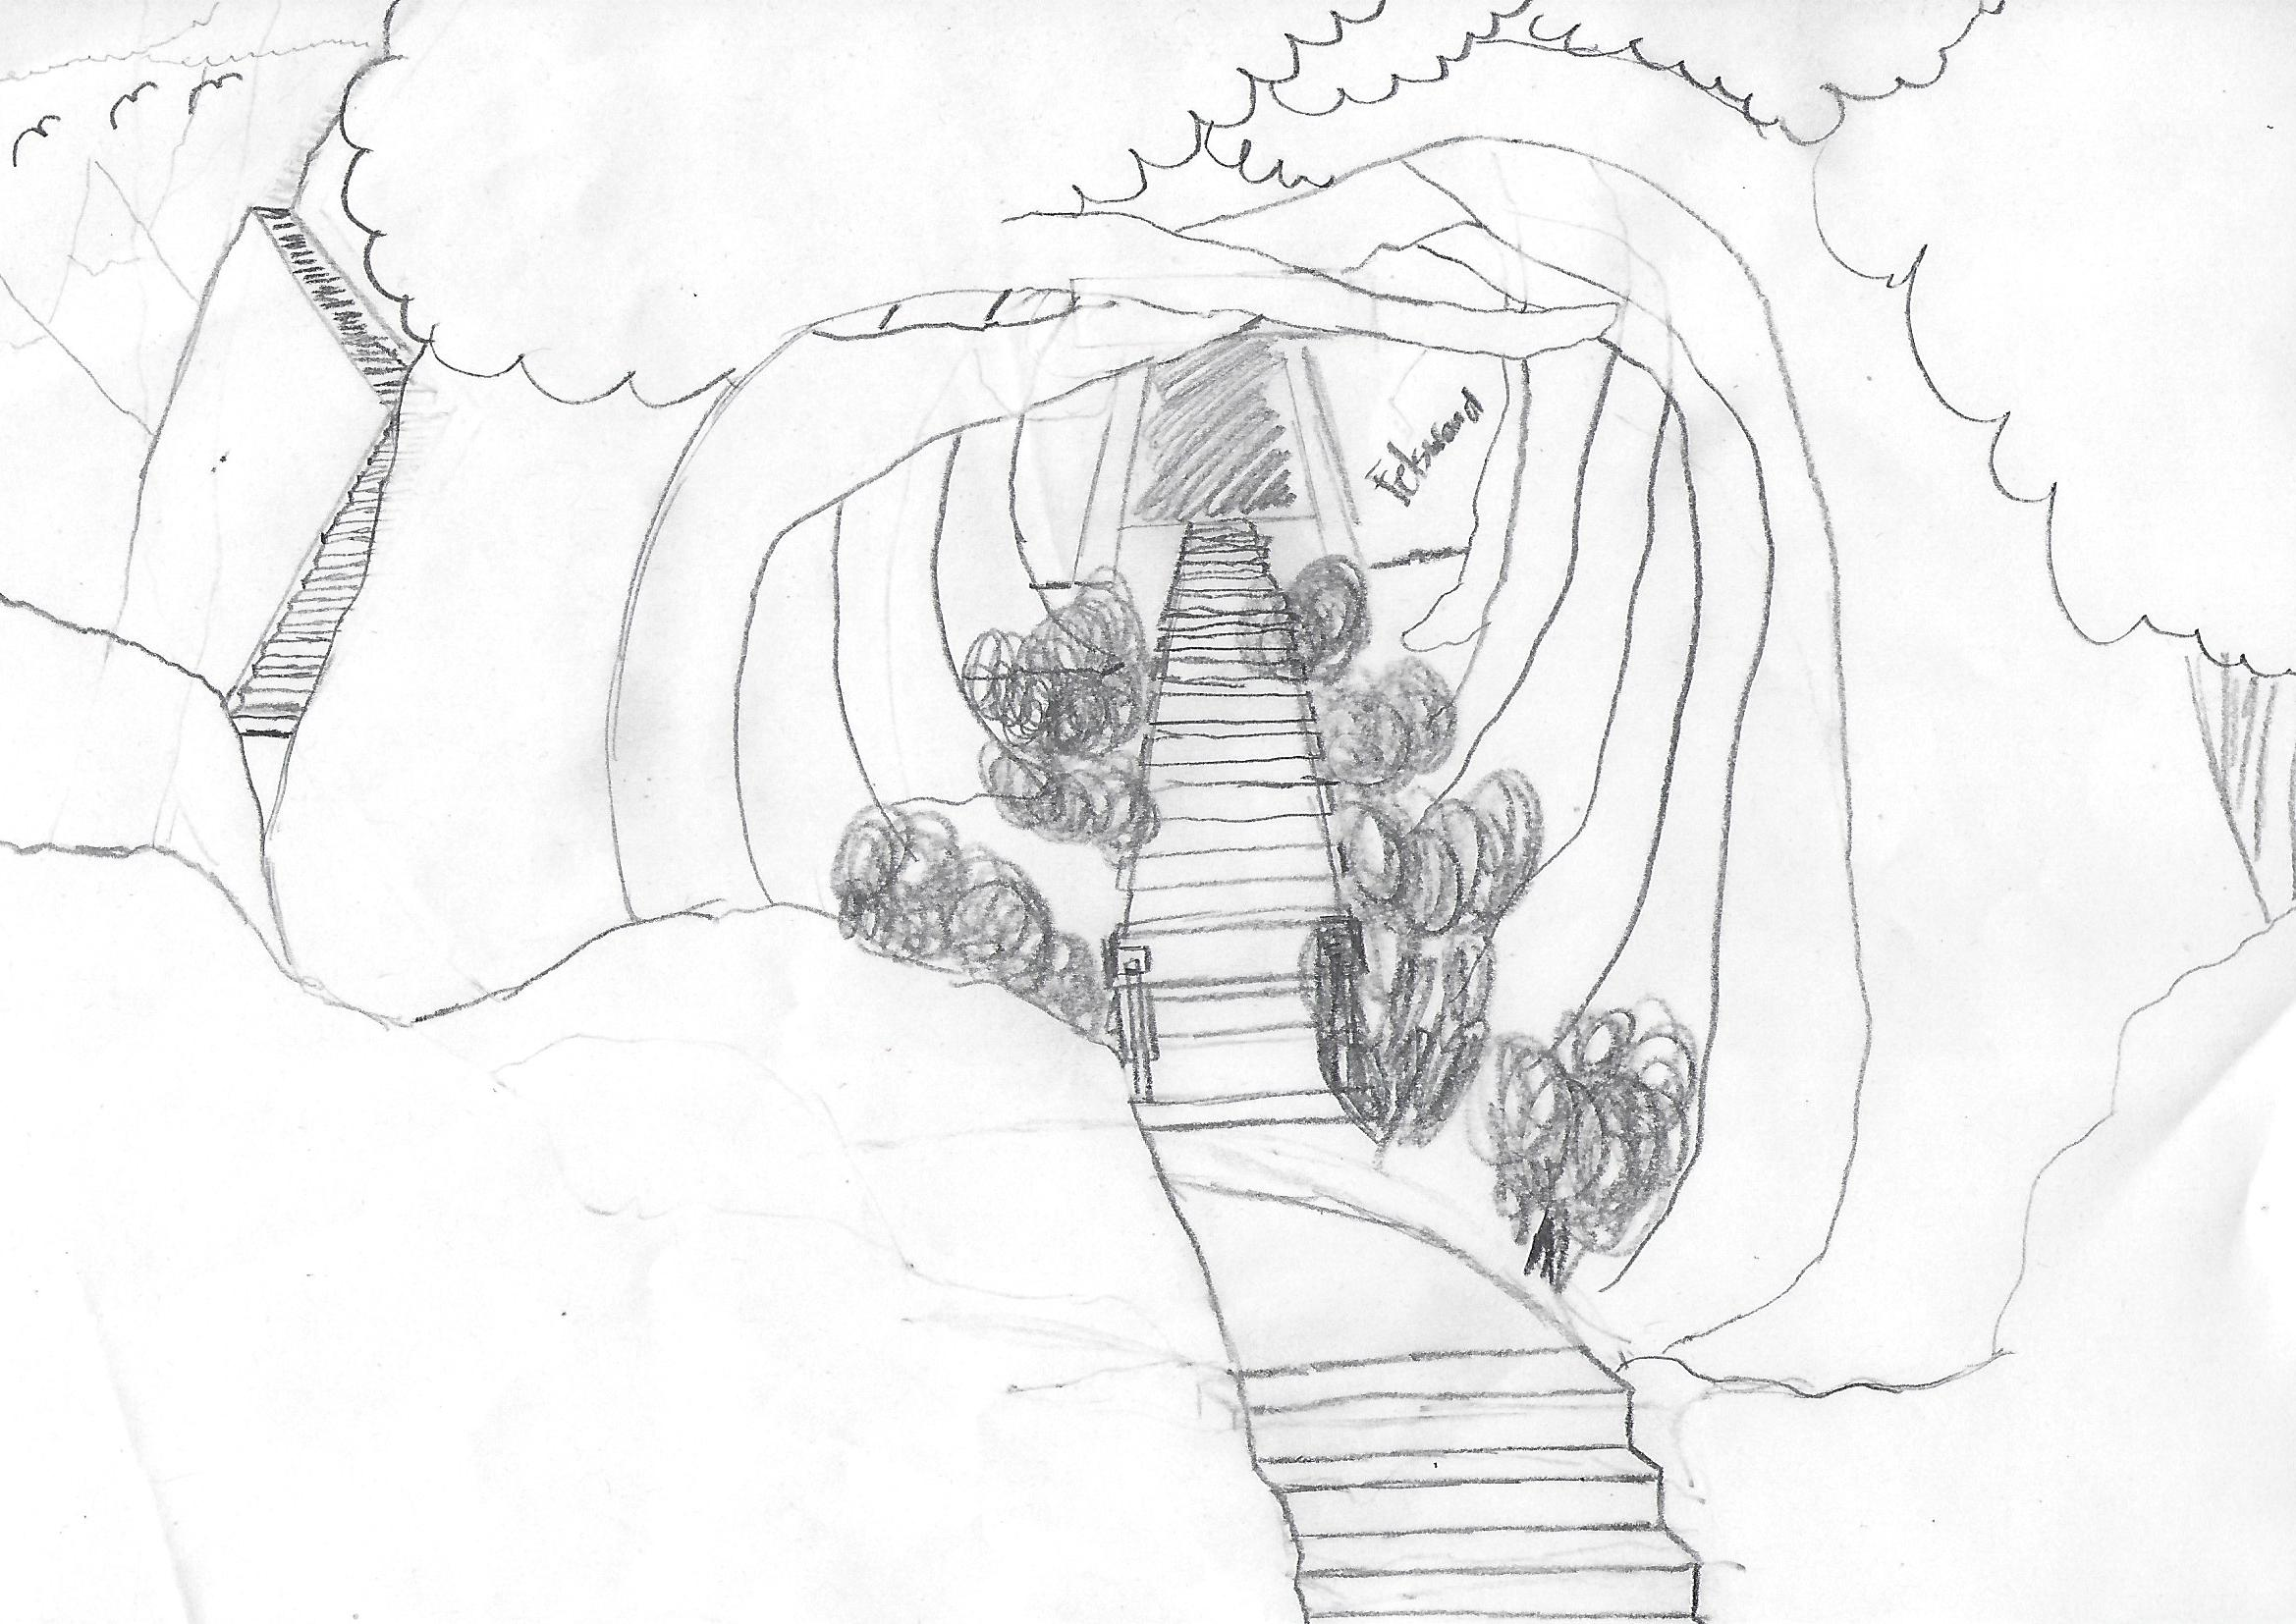
\includegraphics[width=0.5\linewidth]{mine_exterior_concept}}}
  %  \subfloat[][]{\fbox{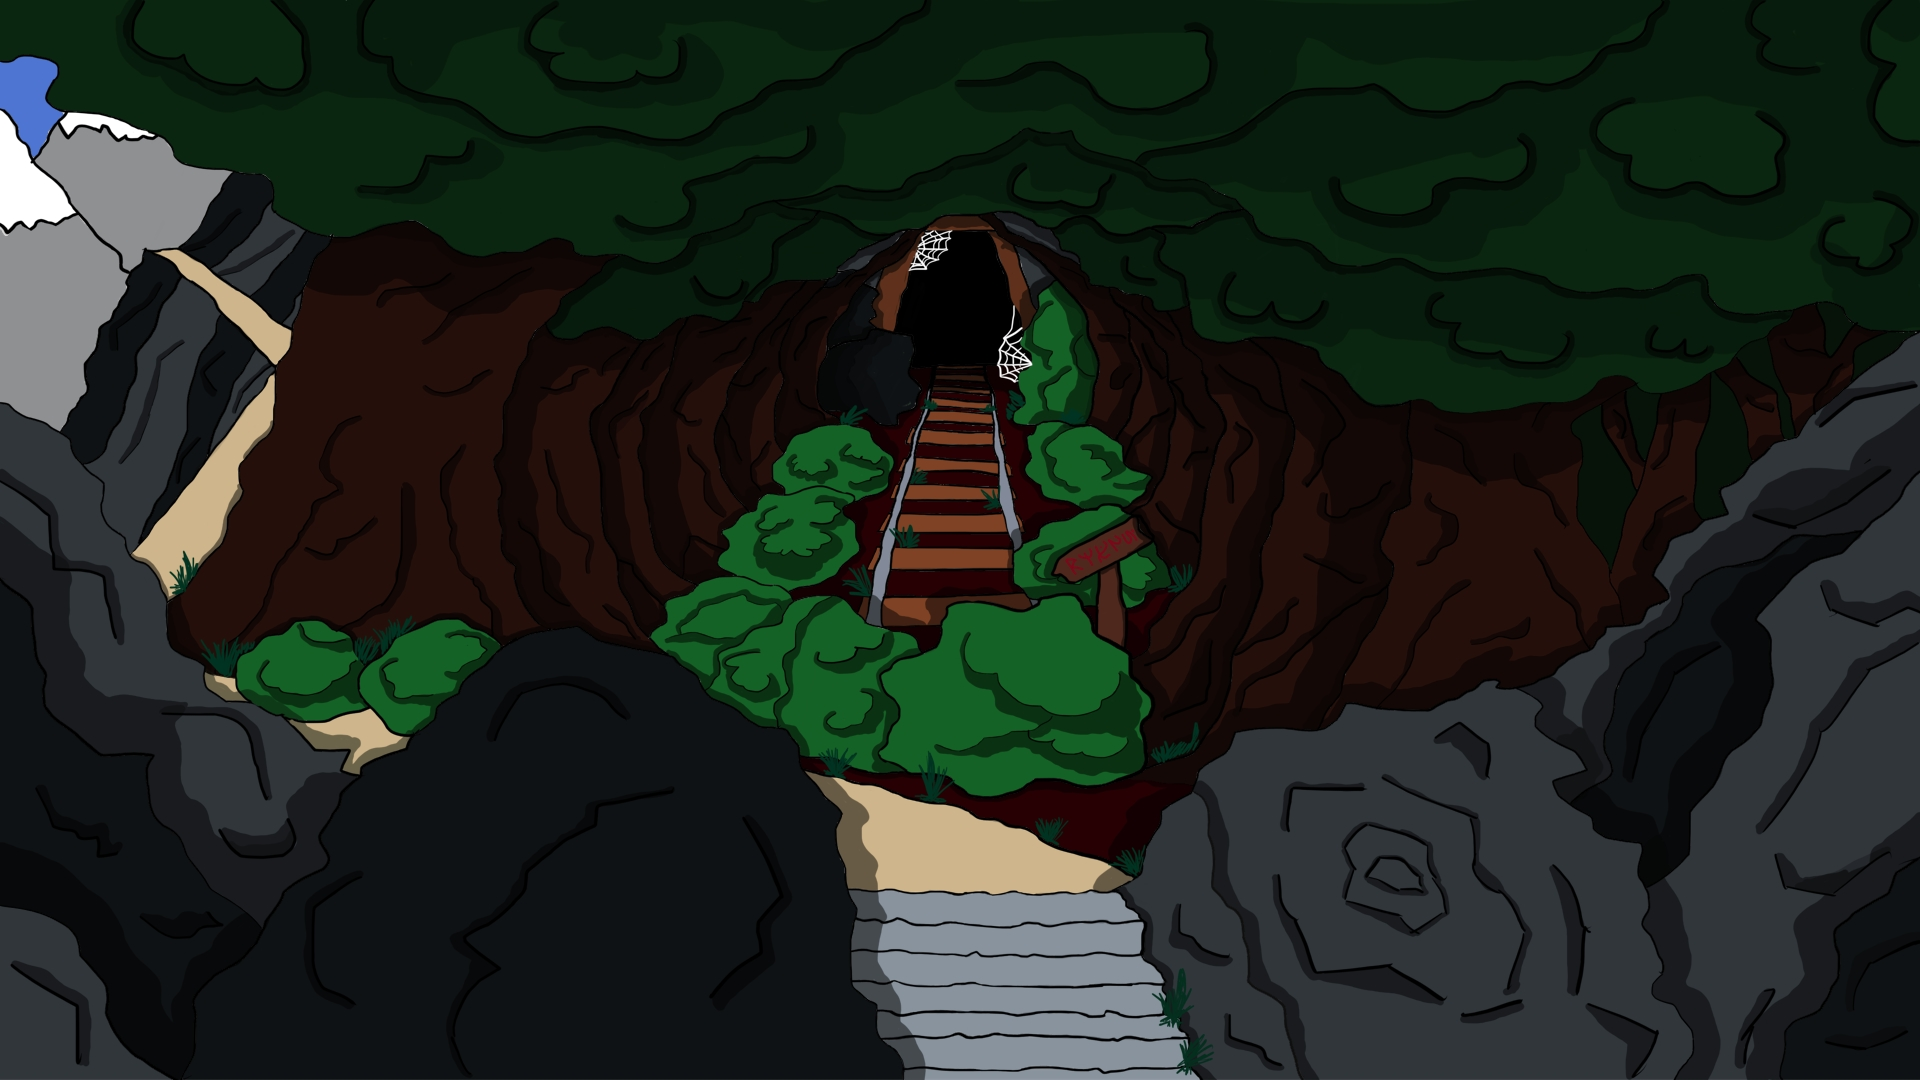
\includegraphics[width=0.5\linewidth]{mine_exterior_final}}}
%\end{figure}

Jede der Spielszenen hat drei Grafik-Assets: eine Intrografik für die Szenenlobby, einen Hintergrund für den Kampfbildschirm und eine Bossgegner-Grafik mit 2D-Animationen. Zudem kommt noch eine weitere Grafik für die Weltkarte hinzu. Diese Letztere, Intro und Hintergrund besitzen das JPG-Bildformat. Die Bossgegner-Grafik dagegen ist ein MP4-Video.
\\Für das JPG-Format entschieden wir uns hauptsächlich auf Grund der im Vergleich zu PNG geringeren Dateigröße. Da es sich bei allen Grafiken, um rein statische Bilder handelt, erschien der Komprimierungsverlust von jpg vernachlässigbar. Zudem wurde für die Bilder keine Hintergrund-Transparenz benötigt.
Alle Grafiken wurden in einer Auflösung von 3840x2160 (Ultra-HD) gezeichnet und dann entweder so verwendet oder auf 1920x1080 (Full-HD) herabskaliert. 

Für die Erstellung der Grafik-Assets und Animationen wurden das freie Zeichen- und 2D-Animationsprogramm \textit{Krita}\footnote{siehe https://krita.org/en/} und ein Grafiktablet verwendet (in der folgenden Abbildung beispielhaft das Standard-UI von Krita).   

\begin{figure}[H]
    \centering
    \caption{Krita Standard-UI}
    \label{fig:krita_ui_example}
    \fbox{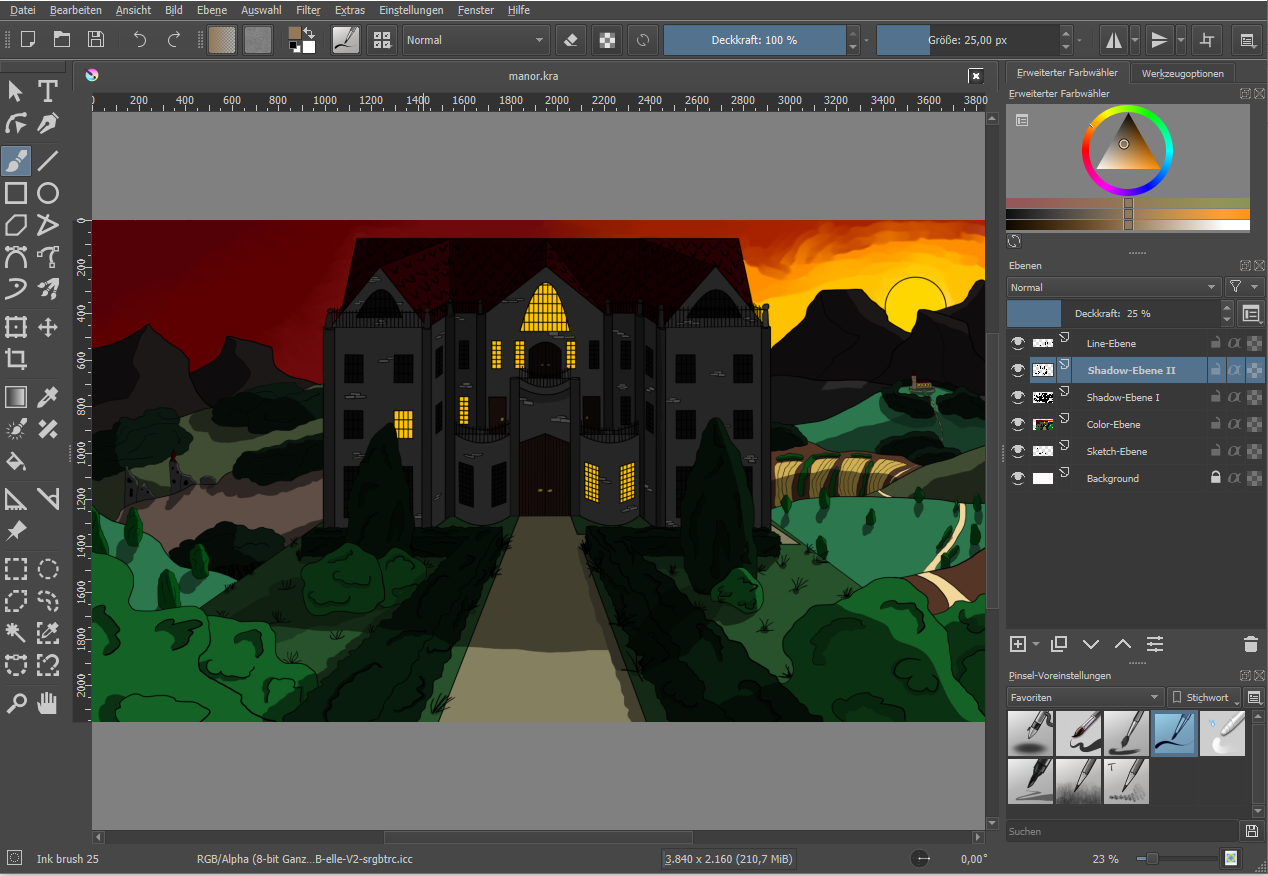
\includegraphics[width=1\textwidth]{krita_ui_example}}
\end{figure}

Die Grafiken wurden hierbei mithilfe der softwareeigenen Ebenenhierarchie systematisch wie folgt aufgebaut: 

Eine Konzeptzeichnung bildet die unterste Ebene mit einer vergleichsweise geringen Deckkraft (\enquote{Sketch-Ebene}). Darüber folgt die \enquote{Linien-Ebene}, auf der auf Basis der Skizze eine vollständige Strichzeichnung mit maximaler Deckkraft angefertigt wird. Diese bildet die oberste Ebene und alle folgenden Ebenen werden aufsteigend zwischen diesen beiden positioniert. Durch eine sorgfältige Linienführung auf dieser Ebene kann das Fülltool auf der nun folgenden \enquote{Farb-Ebene} effektiv genutzt werden. Den Abschluss bilden ein oder zwei \enquote{Schatten-Ebenen}, die mit einer Deckkraft von 50\% bzw. 25\% über der eigentlichen Kolorierung liegen. 

Im Falle der Bossgegner-Grafiken wird dieses Konzept noch um drei Gruppen ergänzt, welche jeweils alle Ebenen in sich zusammenfassen. Es gibt eine Gruppe für das Hintergrundbild, eine Gruppe für die nicht-aninimierten Teile des Bossgegners und eine Gruppe für die eigentlichen Animationen.
Zum Vergleich ist im Folgenden eine Abbildung dieses Aufbaus zu sehen (hier beispielhaft eine Grafik mit 2D-Animation):

\begin{figure}[H]
    \centering
    \caption{Ebenenkonzept für die Grafiken}
    \label{fig:krita_layer_example}
    \fbox{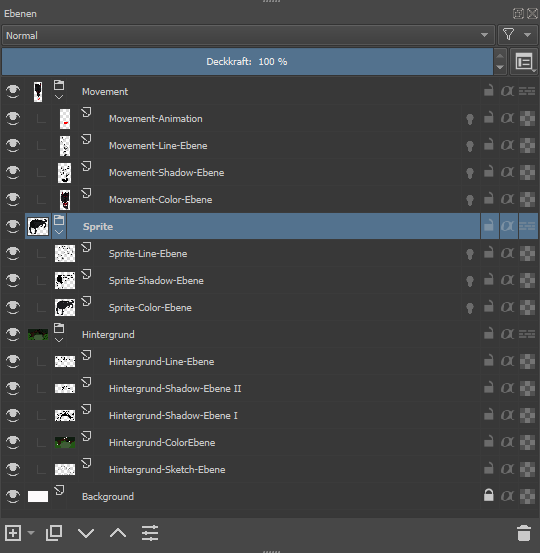
\includegraphics[width=0.7\textwidth]{krita_layer_example}}
\end{figure}

\pagebreak
Dieses Konzept brachte eine erhebliche Flexibilität mit sich. Es war uns damit möglich effizient Änderungen an separaten Teilen der Grafiken durchzuführen, mit der Farbgebung zu experimentieren und nachträglich neue Details einzubringen. Zudem konnten Hintergrundbilder und Bossgrafiken als eine Datei erstellt werden und dann durch Ausblenden verschiedenener Ebenen individuell exportiert werden. Auch der Animationsprozess wurde durch diese Technik deutlich erleichtert. 

Für die Realisierung der 2D-Animationen bietet \textit{Krita} ein dediziertes User-Interface (siehe Abbildung unten). Die Ebenen können hier je nach Bedarf zusammen oder einzeln animiert werden. Dazu werden sie unabhängig voneinander in die Animationsframes kopiert und gegebenenfalls verändert. Im unten zu sehenden Beispiel werden die Ebenengruppen \enquote{Sprite} (nicht-animierter Teil der Bossgegner-Grafik) und \enquote{Movement} (eigentliche Animation) über 10 Frames hinweg durch sukzessive Erhöhung der Deckkraft eingeblendet, um den Effekt eines plötzliches Erscheinens aus Unsichtbarkeit zu erzielen. Danach wird in der \enquote{Movement}-Gruppe über 29 Frames eine Flügelbewegung realisiert. Die Animation wurde dann mit einer Bildwiederholrate von 10 Frames per Second gerendert und als MP4-Video in Ultra-HD und Full-HD exportiert. 

\begin{figure}[H]
    \centering
    \caption{Krita Animation UI}
    \label{fig:krita_animation_example}
    \fbox{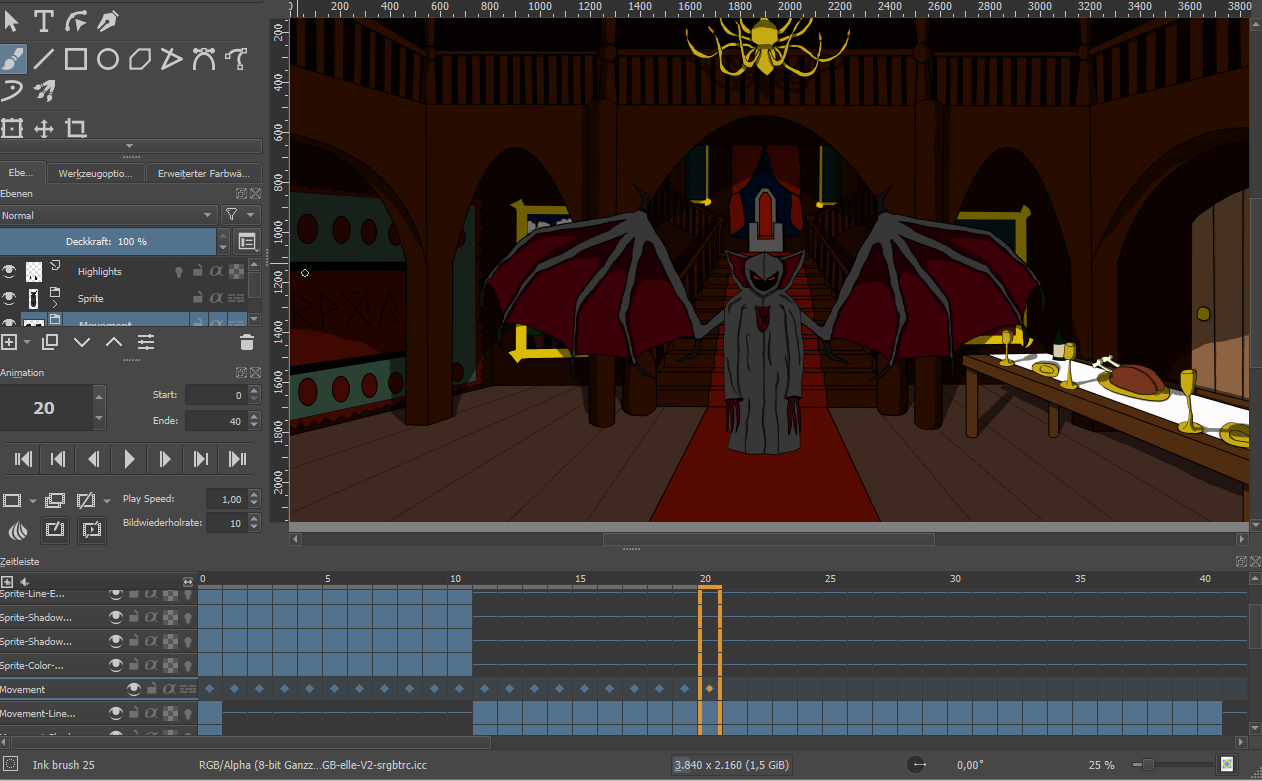
\includegraphics[width=1\textwidth]{krita_animation_example}}
\end{figure}

Die Separierung der Grafiken in animierte und nicht-animierte Teile, stellte bei der eigentlichen Animation eine erhebliche Arbeitserleichterung dar. Viele Veränderungen konnten durch verschieben vorher definierter Abschnitte erreicht werden und mussten nicht pro Frame neu gezeichnet werden (teilweise wurde dies aber trotzdem nötig). Aufgrund des trotz diesen Vorteils immer noch erheblichen Arbeitsaufwandes für vergleichsweise wenige Frames, entschieden wir aber es bei eher rudimentären Animationen zu belassen. Eine Realisierung in 30 Frames per Second beispielsweise wäre and dieser Stelle unverhältnismäßig aufwendig gewesen.

\subsection{Frontend-Design}
    - Design
        - Stil (8-Bit Ära RPG/Adventure)
        - CSS Framework
        - Aufbau des Frontends (HTML-Seiten)
        - Design der einzelnen Seiten 

    - Technisches
        - Worldmap Areas -> SVG-Grafiken

    
\newpage


\section{Reflektion}
(TODO!): Jeder einen Punkt ausschreiben. 

3-4 gute Beispiele, max 1-2 Seiten

\begin{itemize}
    
    \item Umänderung Spielkonzept von Szenenbasiertem Gameplay (Verschiedene Wege, Adventuremäßig, Dialoge, ...) hin zu reinem Kampf-RPG.  
    
    \item Julian...

    \item \textbf{Rundenbasierter vs. chaotischer Spielablauf:} Der Ansatz die Entwicklung durch den Einsatz eines rundenbasierten Ablaufs bzw. Kampfsystems deutlich zu vereinfachen, muss wohl nach den Entwicklungen vom 27.12.2021 (\ref{ref-runden-impl}) zumindest angezweifelt werden. Denn der Aufwand, der durch die notwendige Konzeptionierung und Detailplanung entsteht ist nicht zu unterschätzen. Demengegen stünde bei einem chaotischen Spielablauf lediglich das Handling der Events. 

    \item \textbf{Kleinteilige Aufgabenpakete:} In der Entwicklung eine überschaubare Anzahl an kleinteiligen bzw. Teilufgaben vor sich zu haben, empfand Henning als sehr hilfreich. Man hat damit einen Überblick über die Arbeit der nächsten Tage. Bei der Entwicklung der Rundenlogik entstand durch die Kenntniss um die nächsten Rundenschritte hier ein stets guter Überblick. Der Abschluss jeder einzelnen Teil-Aufgabe sorgte weiter laufend für postive Motivation.

    \item \textbf{Lernkurve und Codequalität:} Eigentlich müsste am Ende eines Entwicklungs-Projektes stets noch einmal von vorne anfangen. Das allein um alles zu korrigieren und anzupassen bzw. auf einen gleichen Quaitätsstand zu bringen, was im Projektverlauf bei den Beteiligten an Fähigkeiten und Wissen gelernt wurde.
    

\end{itemize}






%-----------------------------------
% Apendix / Anhang
%-----------------------------------
\newcommand{\AppendixName}{Anhang}
\newpage
\section*{\AppendixName} %Überschrift "Anhang", ohne Nummerierung
\addcontentsline{toc}{section}{\AppendixName} %Den Anhang ohne Nummer zum Inhaltsverzeichnis hinzufügen

\begin{appendices}
% Nachfolgende Änderungen erfolgten aufgrund von Issue 163
\makeatletter
\renewcommand\@seccntformat[1]{\csname the#1\endcsname:\quad}
\makeatother
\addtocontents{toc}{\protect\setcounter{tocdepth}{0}} %
	\renewcommand{\thesection}{\AppendixName\ \arabic{section}}
	\renewcommand\thesubsection{\AppendixName\ \arabic{section}.\arabic{subsection}}
	


In diesem Abschnitt sind aktuell einige Unterlagen eingefügt, die im Rahmen des Projektes eine Relevanz hatten. Vor Abgabe der Projektarbeit, soll dieser Abschnitt überarbeitet, ausgedünnt und ergänzt werden. 

\section{Projektnotizen}

Austausch und Zusammenarbeite erfolgte auf verschiedenen Platformen:
\begin{itemize}
    \item Gezeichnet und Entwürfe wurden meist in Miro erstellt: \url{https://miro.com/app/board/uXjVOdN2haQ=/}. 
    \item Besprechungen erfolgten meist in Teams: \url{https://teams.microsoft.com/l/team/19%3aDoBvOwOIC6WNhsL9kOIYFKNtVftU1yBtcEn_gcyQtcg1%40thread.tacv2/conversations?groupId=850a22ff-34a2-4fe2-a506-f55ac4d595f8&tenantId=b9b6f99a-a243-422d-ab36-f726574c981a}. 
    \item Der gemeinsame Code und die Dokumentation wurden auf Github erstelt: \url{https://github.com/tstsrv-de/tstsrv-de}. 
\end{itemize}

\subsection{Projektbesprechungen}

Stets Sonntags erfolgten Projektbesprechungen. Notizen und Zusammenfassungen davon finden sich hier in fortschreitender, chronologischer Reihenfolge. Ebenso hier entsprechend einsortiert, finden sich Konzeptzeichnungen und Entwürfe aller Art (UI, Code, Datenbankmodelle).

(TODO!) Bildbeschreibungen ergänzen, wichtige Bilder beschreiben.

2021-11-23-erster-entwurf-gameloop 
\begin{figure}[H]
    \centering
    \caption[]{2021-11-23-erster-entwurf-gameloop}
    \label{fig:2021-11-23-erster-entwurf-gameloop}
    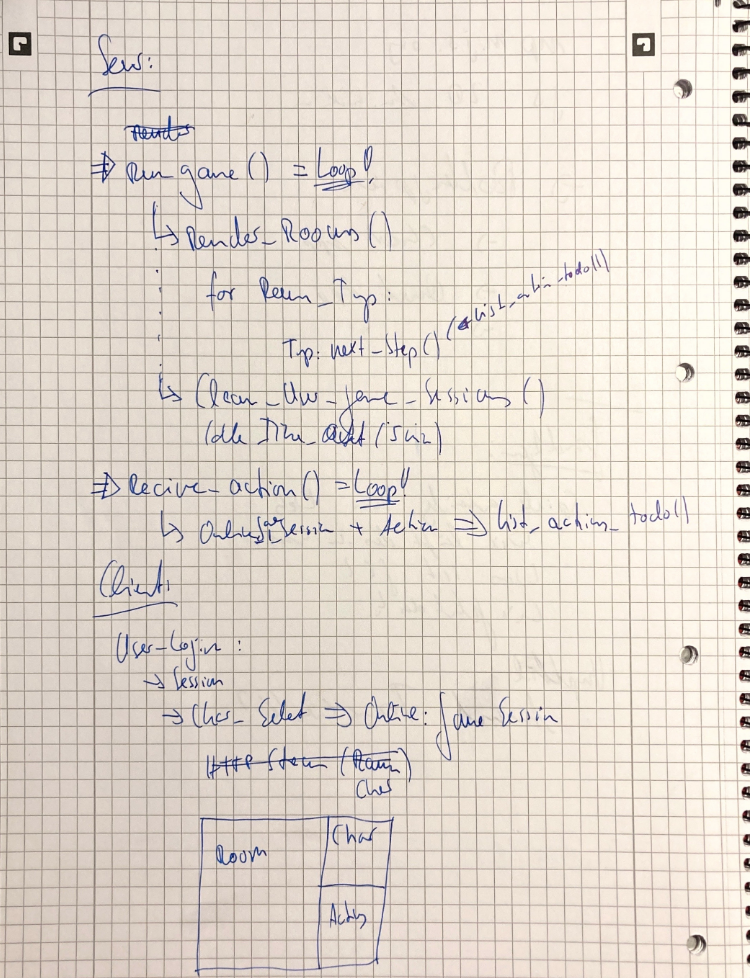
\includegraphics[width=1\textwidth]{2021-11-23-erster-entwurf-gameloop}
\end{figure}

2021-11-23-erstes-db-konzept 
\begin{figure}[H]
    \centering
    \caption[]{2021-11-23-erstes-db-konzept}
    \label{fig:2021-11-23-erstes-db-konzept}
    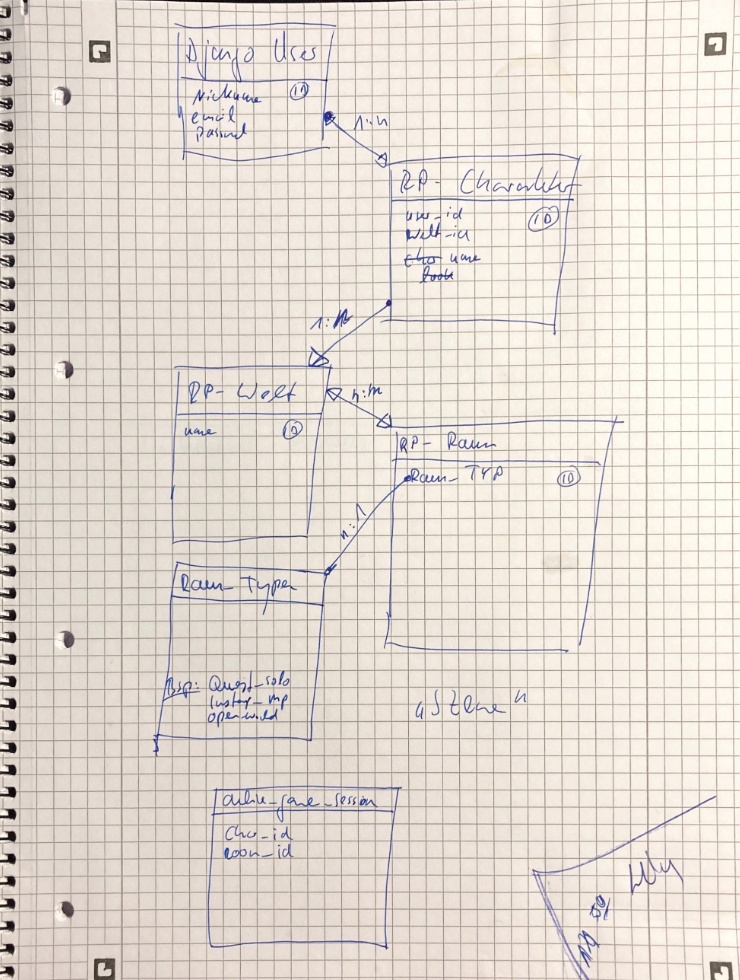
\includegraphics[width=1\textwidth]{2021-11-23-erstes-db-konzept}
\end{figure}

2021-11-27-erstentwurf-ui 
\begin{figure}[H]
    \centering
    \caption[]{2021-11-27-erstentwurf-ui}
    \label{fig:2021-11-27-erstentwurf-ui}
    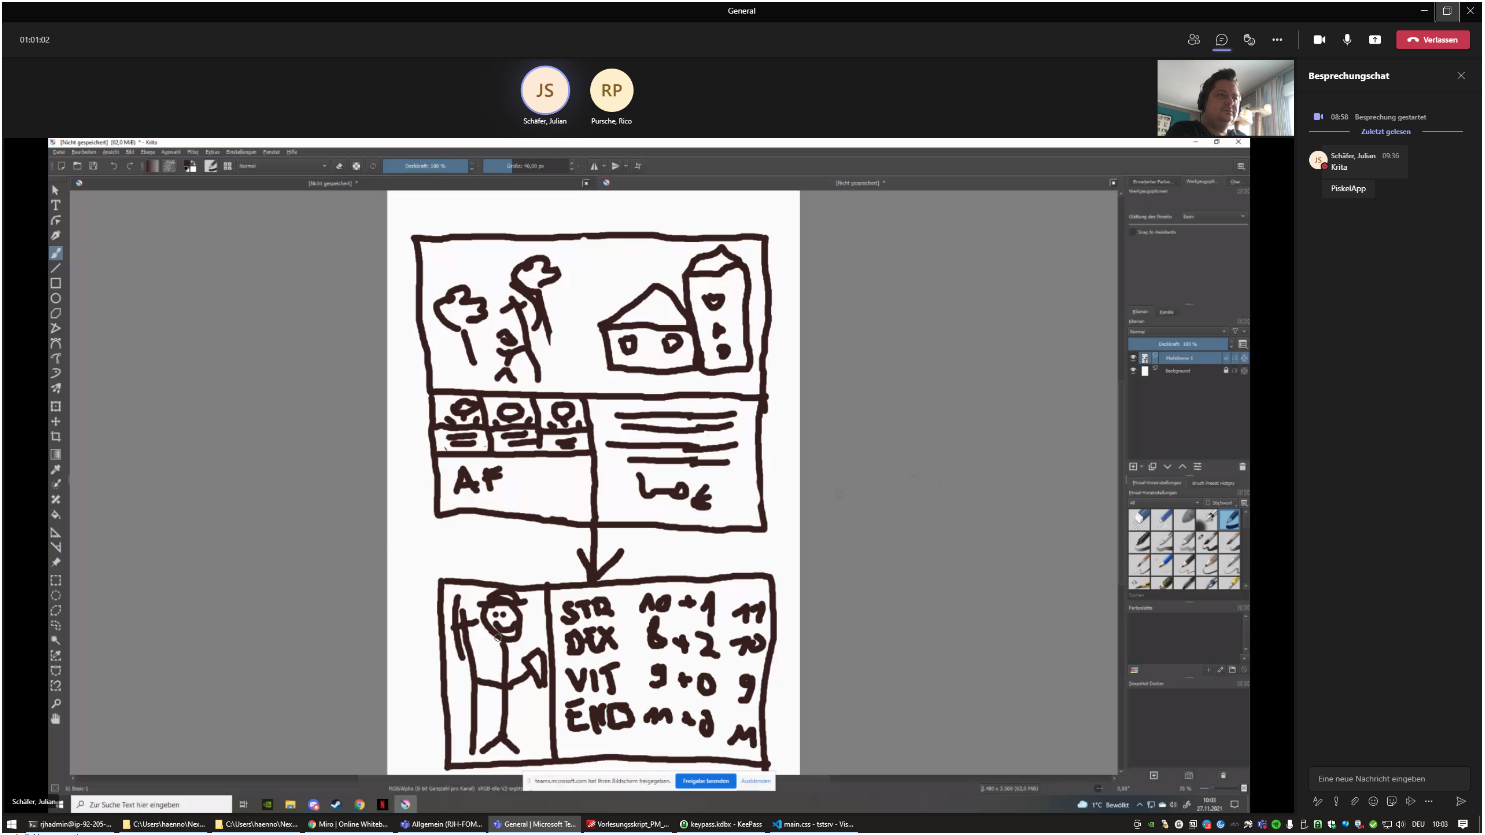
\includegraphics[width=1\textwidth]{2021-11-27-erstentwurf-ui}
\end{figure}

2021-11-27-projektskizze-1 
\begin{figure}[H]
    \centering
    \caption[]{2021-11-27-projektskizze-1}
    \label{fig:2021-11-27-projektskizze-1}
    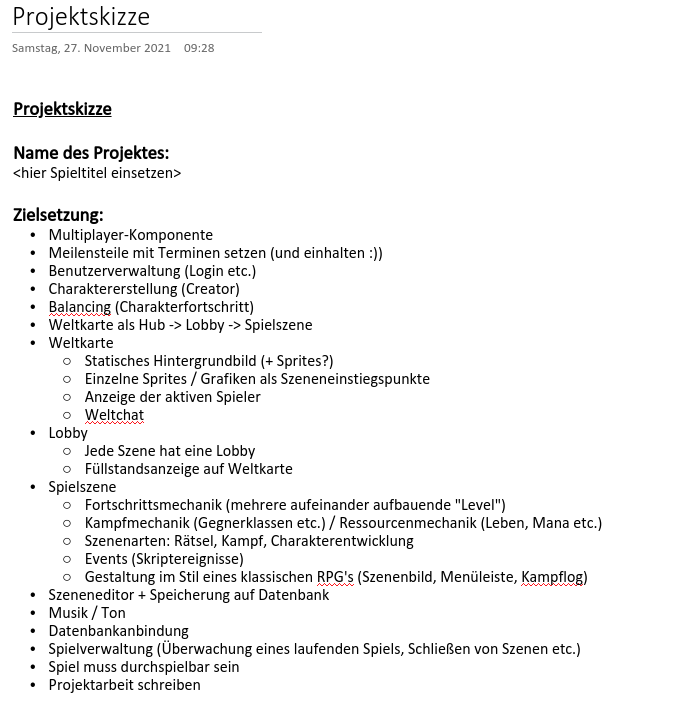
\includegraphics[width=1\textwidth]{2021-11-27-projektskizze-1}
\end{figure}

2021-11-27-projektskizze-2 
\begin{figure}[H]
    \centering
    \caption[]{2021-11-27-projektskizze-2}
    \label{fig:2021-11-27-projektskizze-2}
    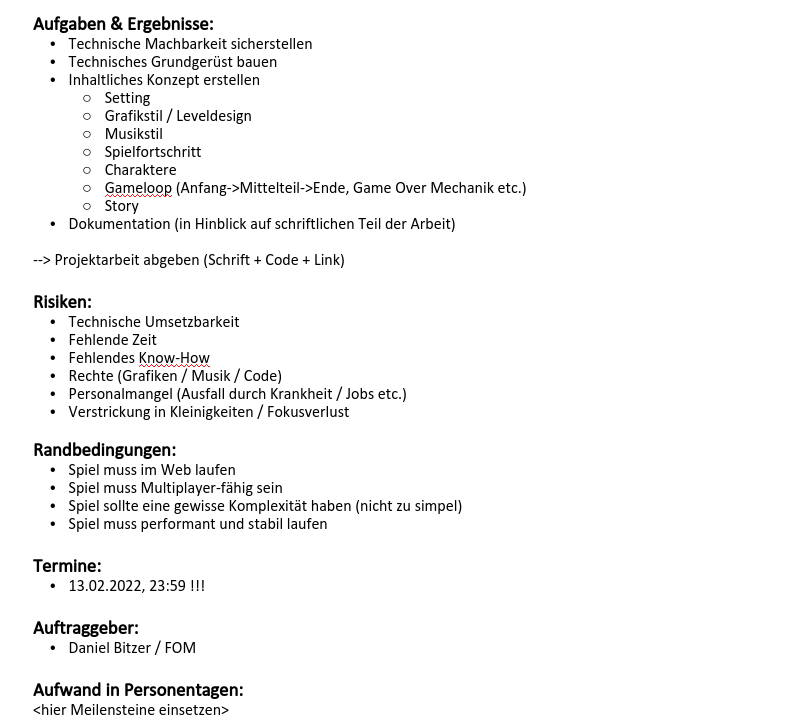
\includegraphics[width=1\textwidth]{2021-11-27-projektskizze-2}
\end{figure}

2021-11-29-Entwurf-Klassen-Ui 
\begin{figure}[H]
    \centering
    \caption[]{2021-11-29-Entwurf-Klassen-Ui}
    \label{fig:2021-11-29-Entwurf-Klassen-Ui}
    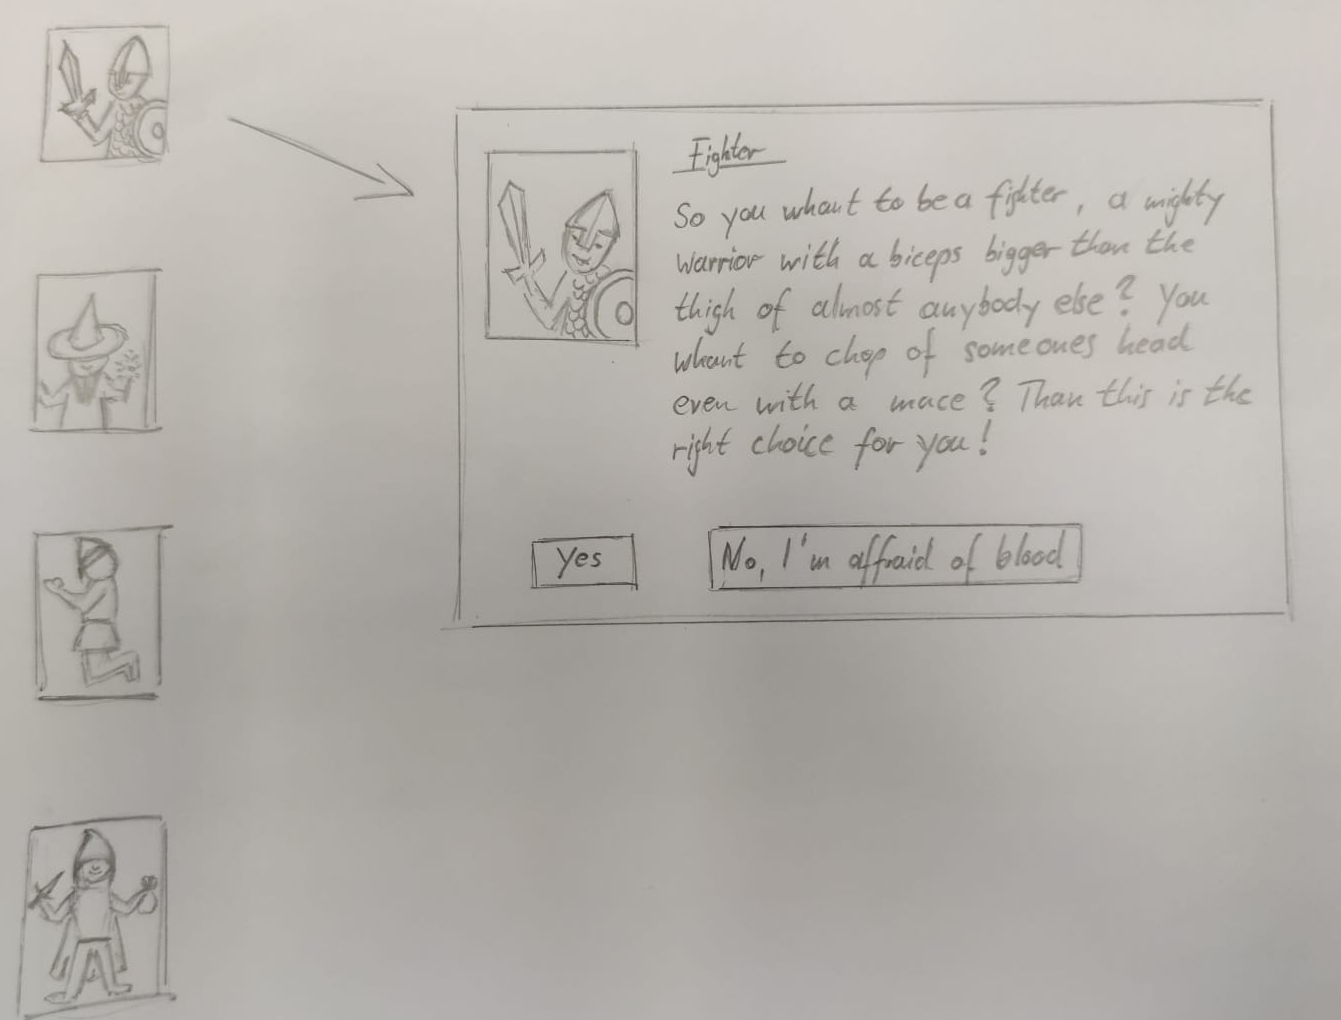
\includegraphics[width=1\textwidth]{2021-11-29-Entwurf-Klassen-Ui}
\end{figure}

2021-11-30-Entwurf-Lobby-Logik 
\begin{figure}[H]
    \centering
    \caption[]{2021-11-30-Entwurf-Lobby-Logik}
    \label{fig:2021-11-30-Entwurf-Lobby-Logik}
    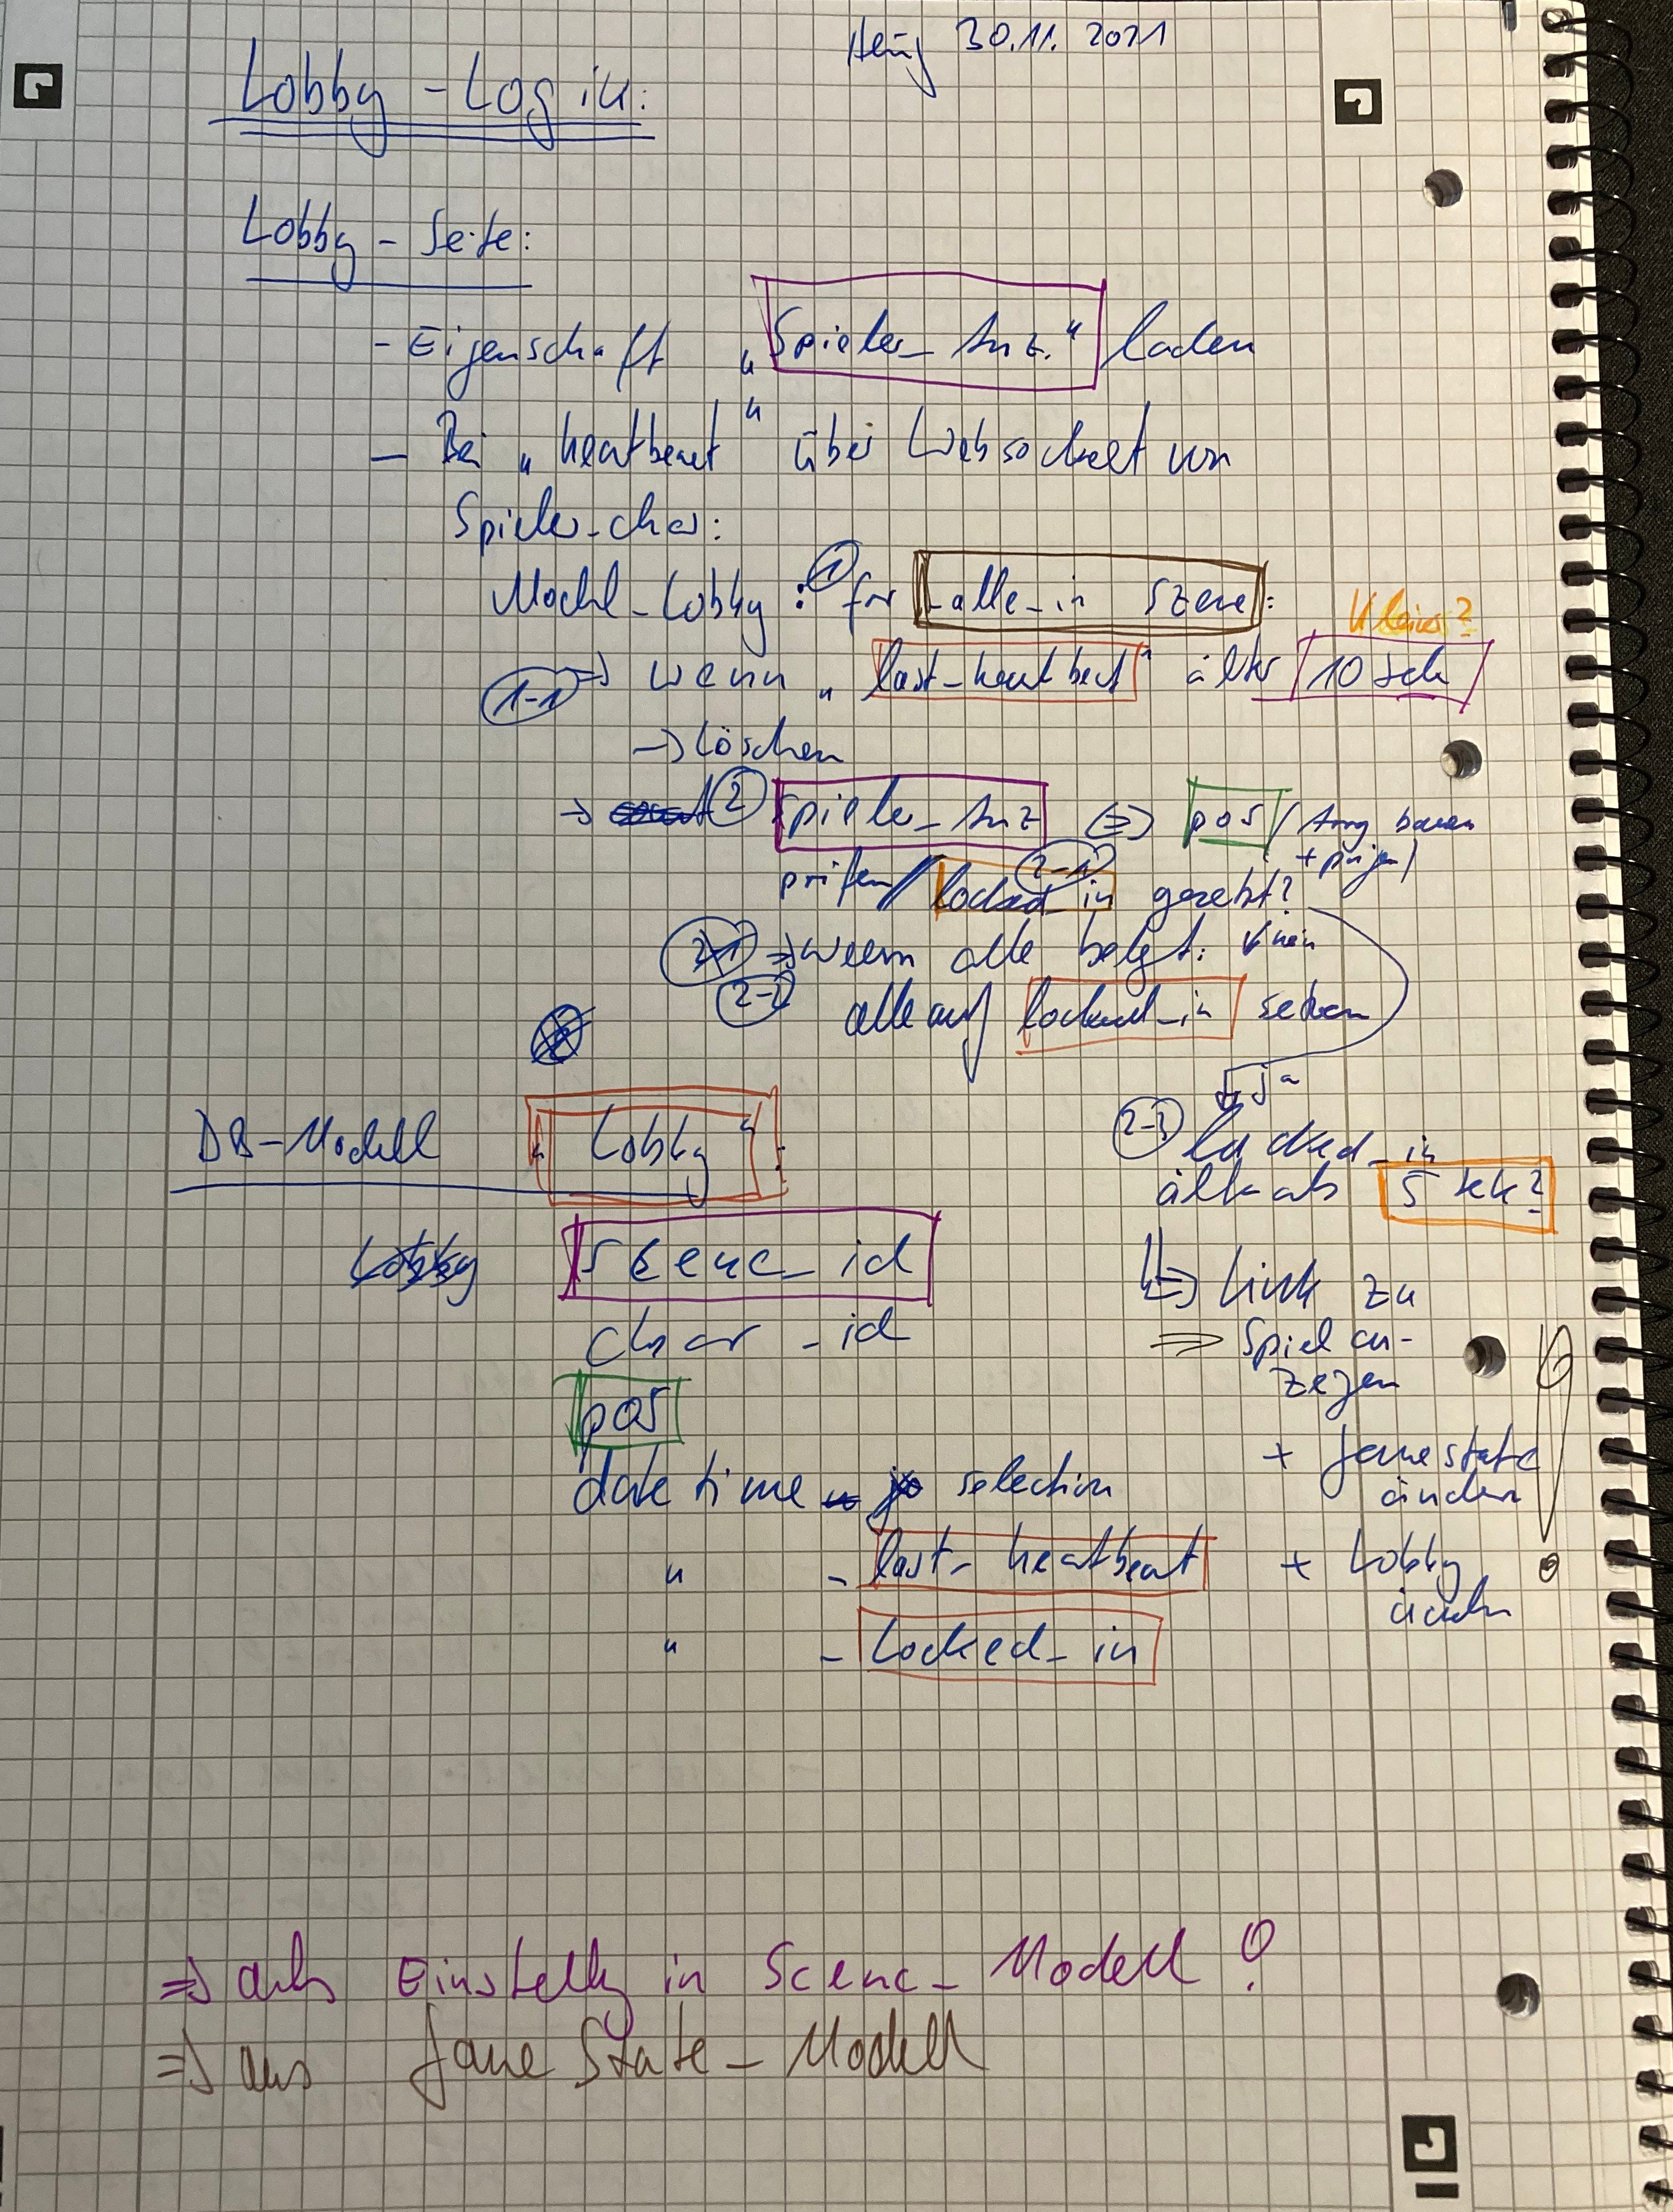
\includegraphics[width=1\textwidth]{2021-11-30-Entwurf-Lobby-Logik}
\end{figure}

2021-11-30-Entwurf-Lobby-UI 
\begin{figure}[H]
    \centering
    \caption[]{2021-11-30-Entwurf-Lobby-UI}
    \label{fig:2021-11-30-Entwurf-Lobby-UI}
    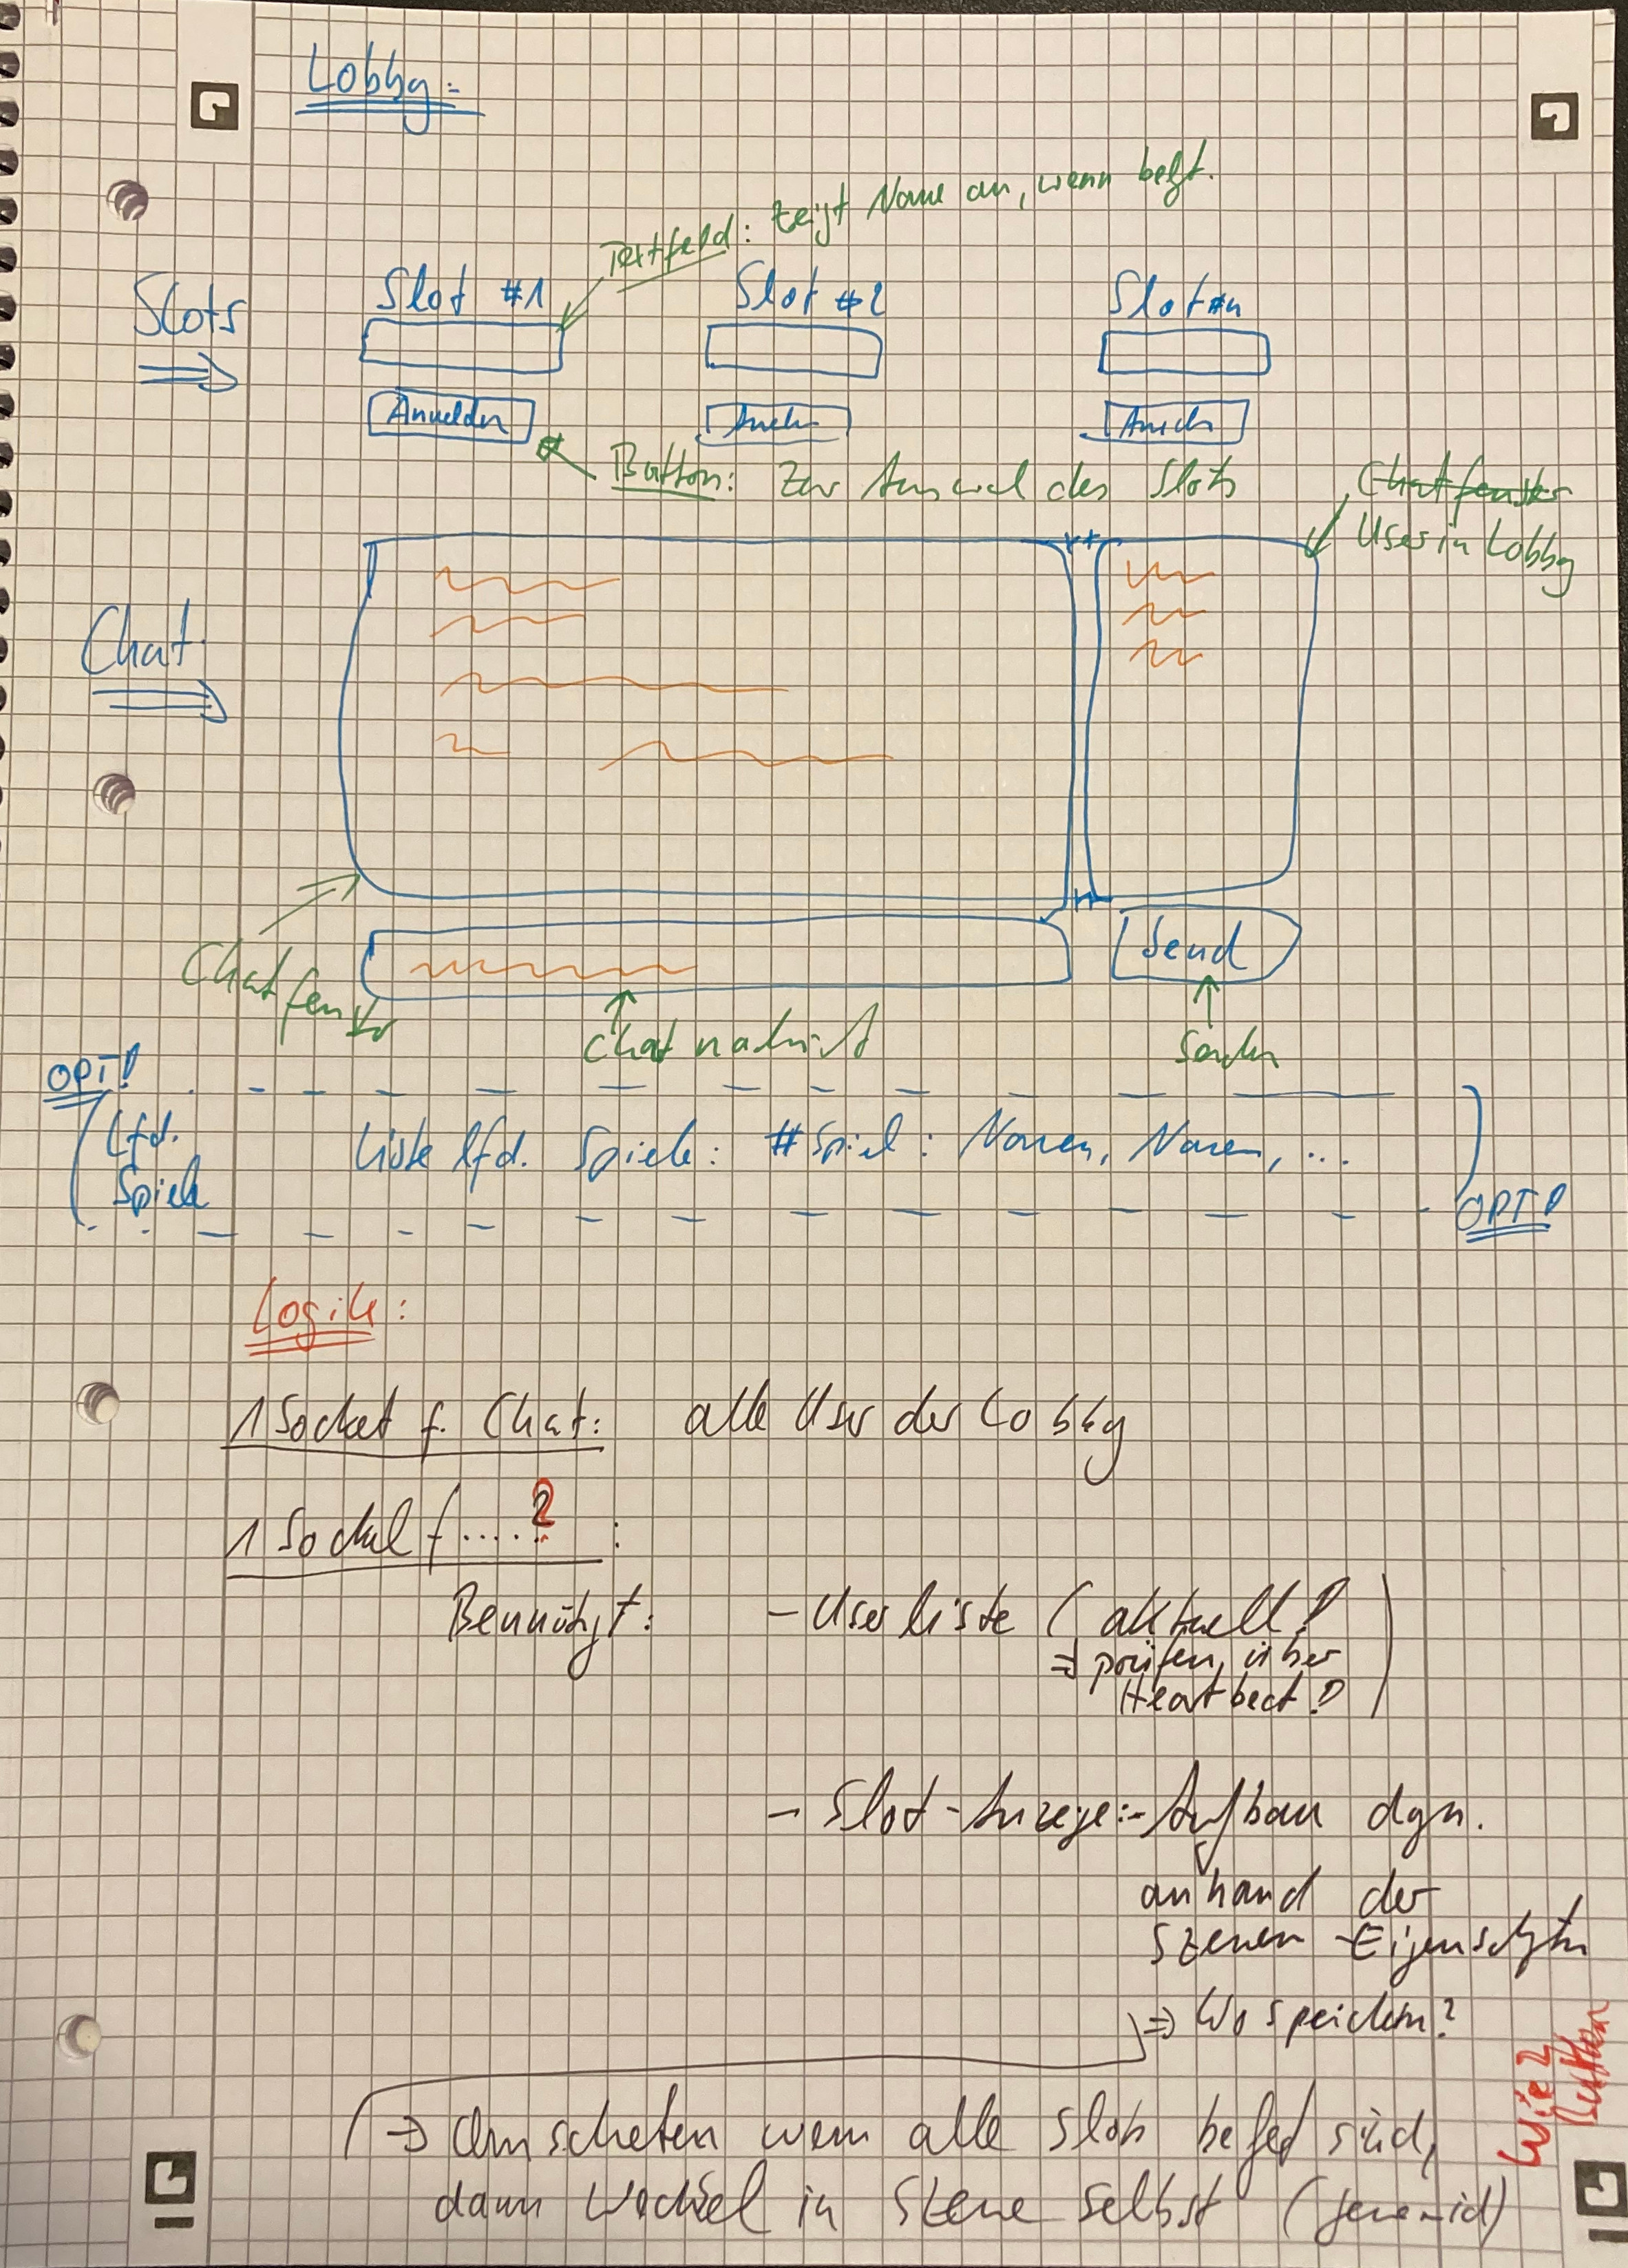
\includegraphics[width=1\textwidth]{2021-11-30-Entwurf-Lobby-UI}
\end{figure}

2021-12-02-Countdown-Logik 
\begin{figure}[H]
    \centering
    \caption[]{2021-12-02-Countdown-Logik}
    \label{fig:2021-12-02-Countdown-Logik}
    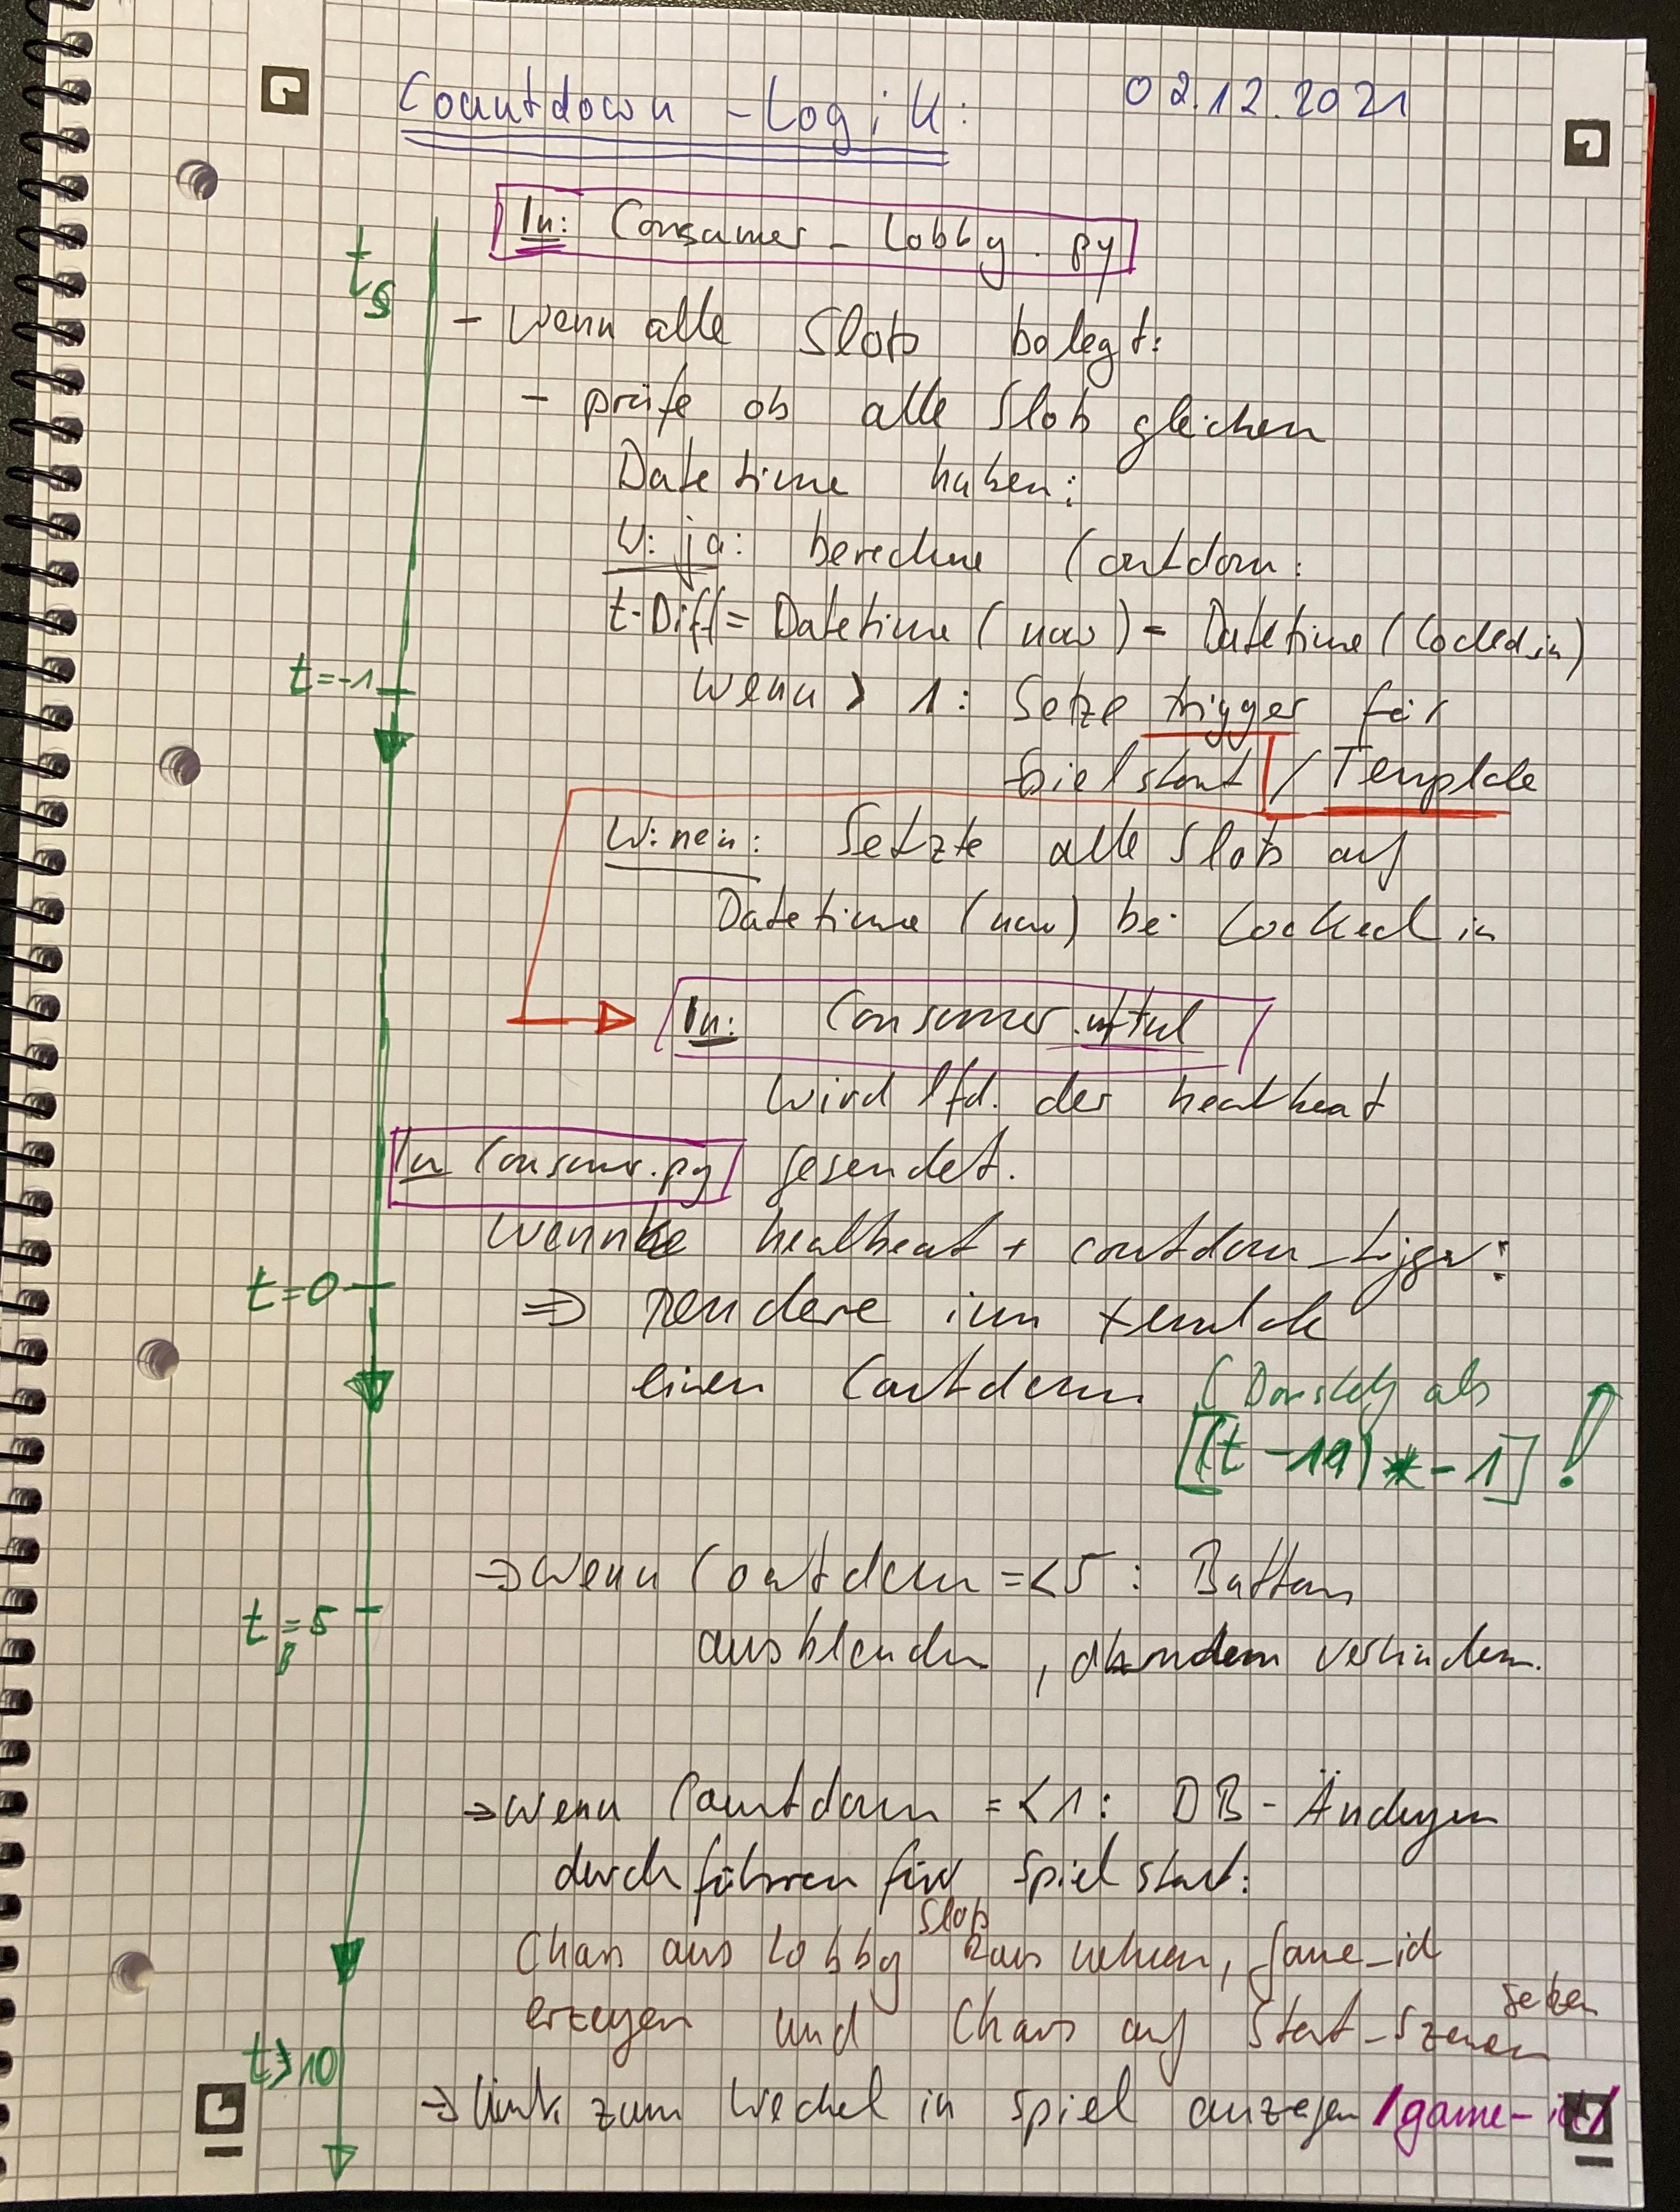
\includegraphics[width=1\textwidth]{2021-12-02-Countdown-Logik}
\end{figure}

2021-12-05-Projketbesprechung-Miro-b 
\begin{figure}[H]
    \centering
    \caption[]{2021-12-05-Projketbesprechung-Miro-b}
    \label{fig:2021-12-05-Projketbesprechung-Miro-b}
    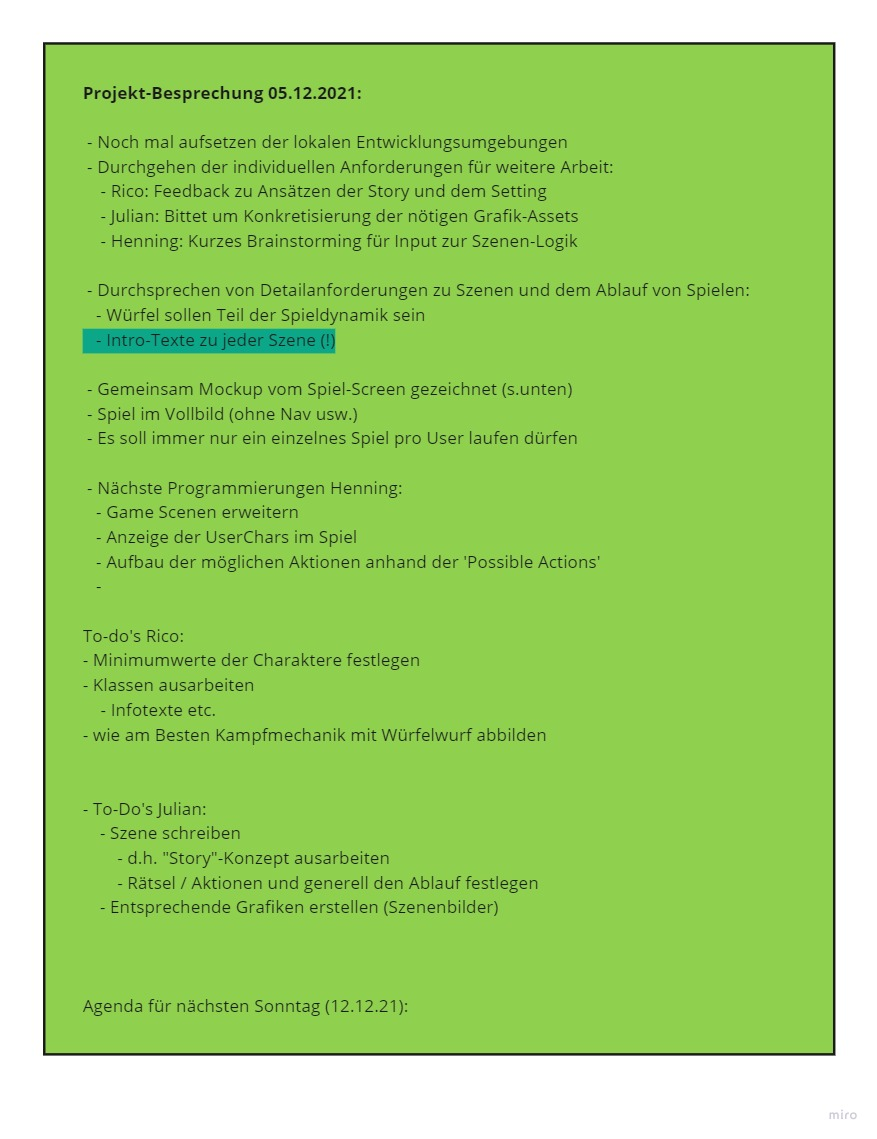
\includegraphics[width=1\textwidth]{2021-12-05-Projketbesprechung-Miro-b}
\end{figure}

2021-12-05-Projketbesprechung-Miro-c 
\begin{figure}[H]
    \centering
    \caption[]{2021-12-05-Projketbesprechung-Miro-c}
    \label{fig:2021-12-05-Projketbesprechung-Miro-c}
    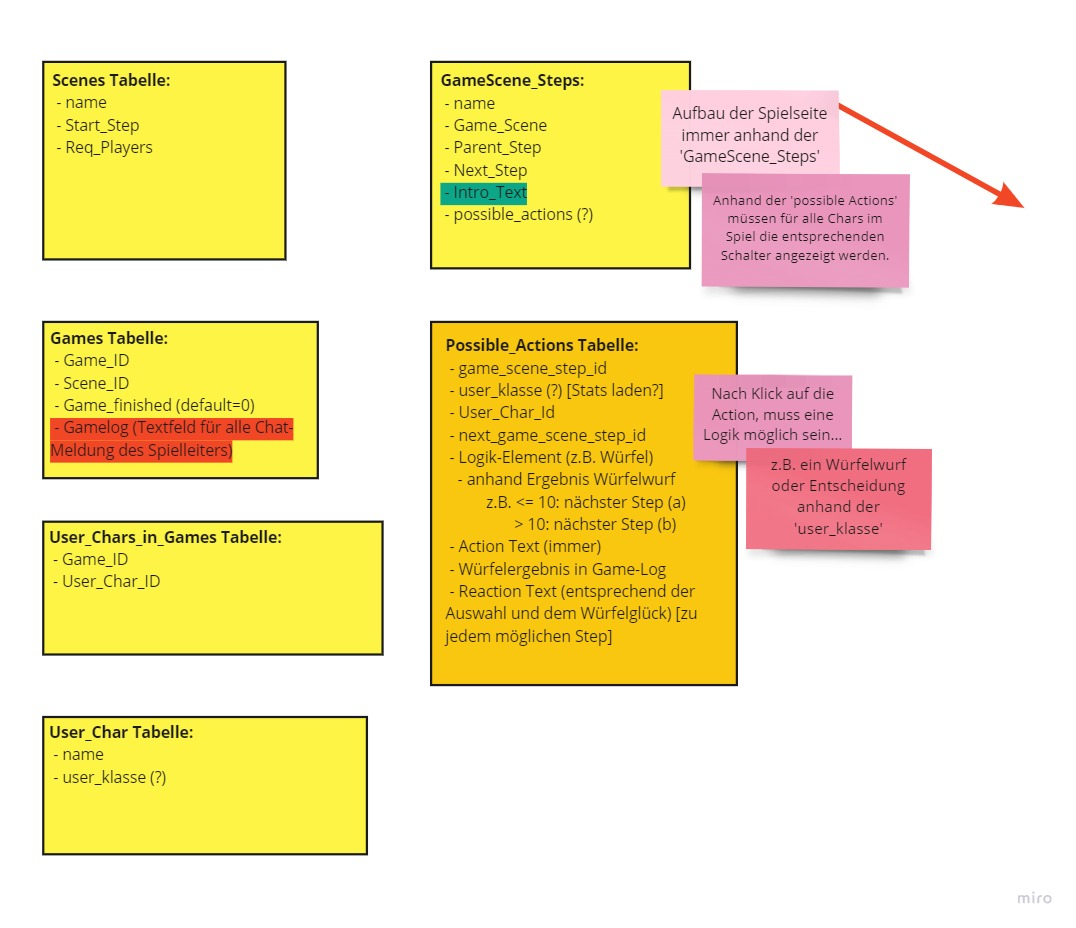
\includegraphics[width=1\textwidth]{2021-12-05-Projketbesprechung-Miro-c}
\end{figure}

2021-12-05-Projketbesprechung-Miro-d 
\begin{figure}[H]
    \centering
    \caption[]{2021-12-05-Projketbesprechung-Miro-d}
    \label{fig:2021-12-05-Projketbesprechung-Miro-d}
    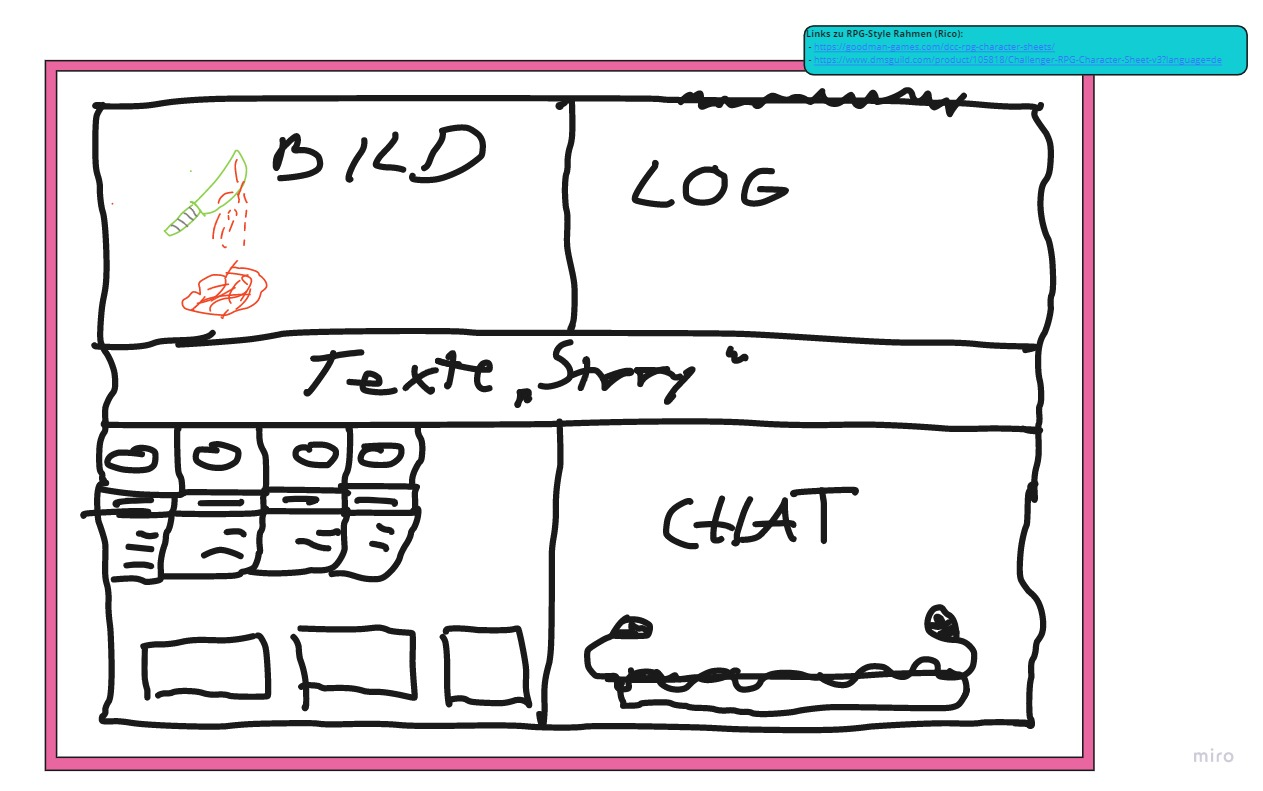
\includegraphics[width=1\textwidth]{2021-12-05-Projketbesprechung-Miro-d}
\end{figure}

2021-12-11-Projekt-Besprechung-Klassenbeschreibung 
\begin{figure}[H]
    \centering
    \caption[]{2021-12-11-Projekt-Besprechung-Klassenbeschreibung}
    \label{fig:2021-12-11-Projekt-Besprechung-Klassenbeschreibung}
    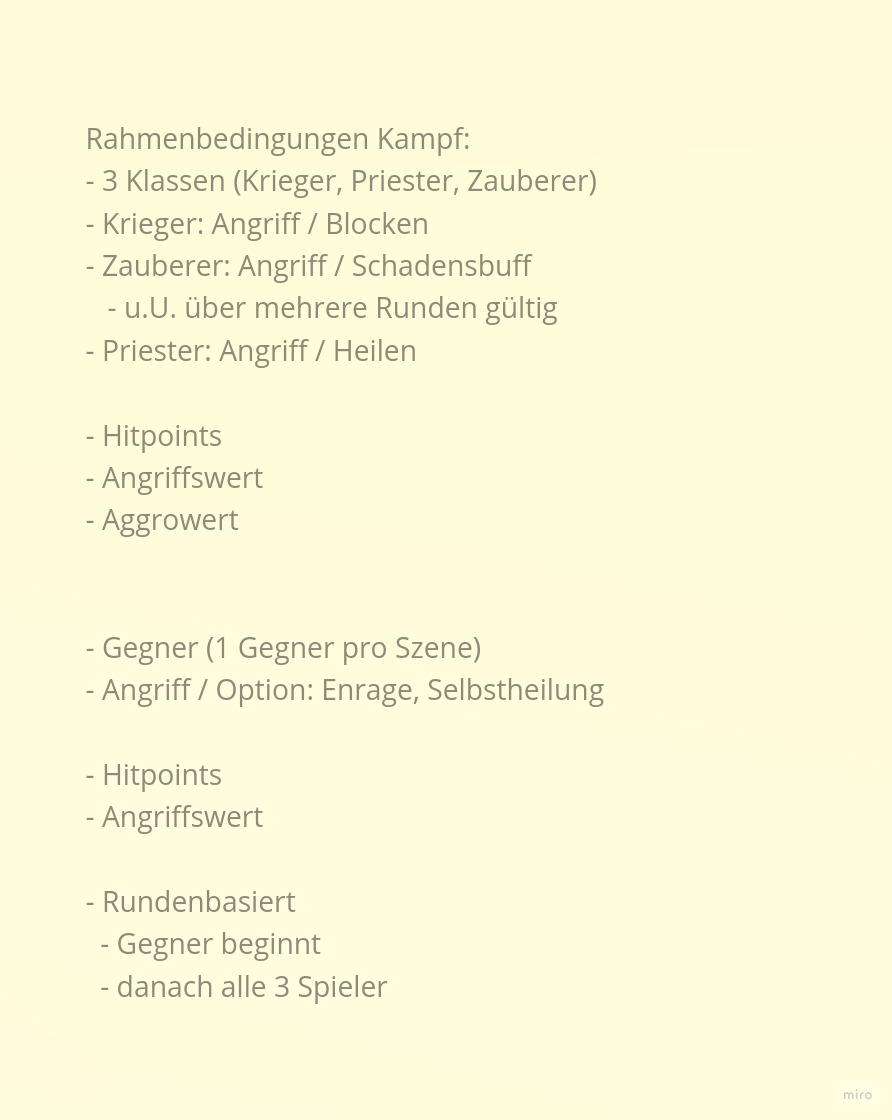
\includegraphics[width=1\textwidth]{2021-12-11-Projekt-Besprechung-Klassenbeschreibung}
\end{figure}


\begin{figure}[H]
    \centering
    \caption[]{11.12.2021: Projekt Besprechung: Gegenseitiges Update und Wechsel von Szenenlogik zu Kampfsystem für das RPG }
    \label{fig:2021-12-11-Projekt-Besprechung}
    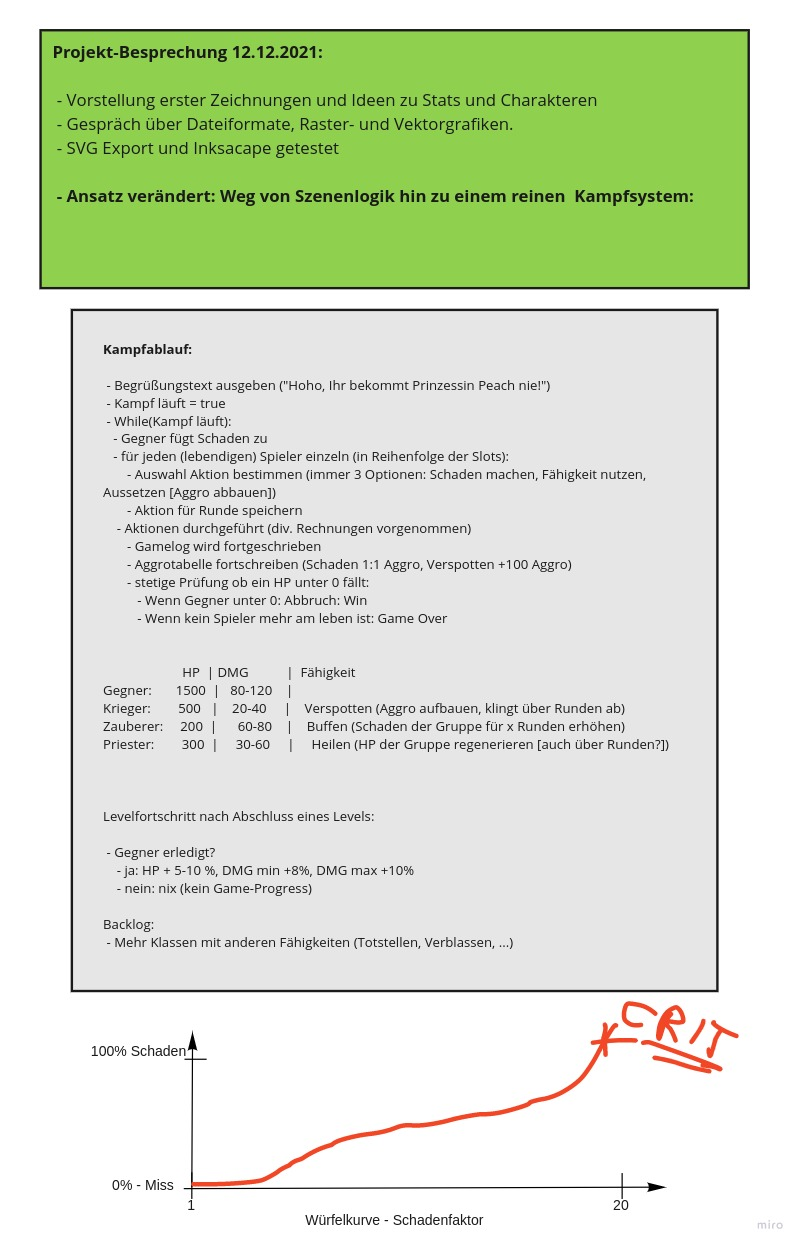
\includegraphics[width=1\textwidth]{2021-12-11-Projekt-Besprechung}
\end{figure}



\section{Entwicklungsnotizen}


\subsection{Enwticklung, Samstag 13.11.2021}

Allererste Tests und Anlage der Django-App sowie  hochladen des ersten Stands zu Github (Commits \url{https://git.io/JSq7n} und \url{https://git.io/JSYH4}). Eigene Notizen zum Ablauf dazu hier: 


\begin{lstlisting}
1. copy files (docker-compose, dockerfile, example.env, requirements.txt) from repo local
2. rename .env.example to .env and change settings 
3. init django with: docker-compose run rpg django-admin startproject rpg .
4. edit rpg/settings.py:
    add:
        start:
            import os
            import environ
            env = environ.Env()
            environ.Env.read_env()
        after 'BASE_DIR':
            TEMPLATES_DIR = os.path.join(BASE_DIR, 'templates')
            STATIC_DIR = os.path.join(BASE_DIR, 'static')
        after STATIC_URL:
            STATICFILES_DIRS = [
                STATIC_DIR,
            ]
    change: 
        SECRET_KEY to:
            SECRET_KEY = env('ENV_SECRET_KEY')
        ALLOWED_HOSTS to:
            ALLOWED_HOSTS = [env('ENV_ALLOWED_HOSTS')]
        in Templates, Dirs to:
                'DIRS': [TEMPLATES_DIR],
        DATABASES to:
            DATABASES = {
                'default': {
                    'ENGINE': 'django.db.backends.postgresql',
                    'NAME': env('ENV_POSTGRES_DB'),
                    'USER': env('ENV_POSTGRES_USER'),
                    'PASSWORD': env('ENV_POSTGRES_PASSWORD'),
                }
            }

5. copy and rename .env.example also to rpg/.env (remeber to copy again @changes)
6. update django to new db: 'docker-compose run python manage.py makemigrations' and 'docker-compose run python manage.py migrate'
7. create superuser: docker-compose run rpg python manage.py createsuperuser
8. create django app: docker-compose run rpg python manage.py startapp rjh_rpg 
\end{lstlisting}




\subsection{Enwticklung, Mittwoch 24.11.2021}

Einbau von Grundlagen: 
\begin{itemize}
    \item Update der Django-Basis Installtion bzw. des Projektes (Commit \url{https://git.io/JSqbt}). 
    \item Einbau der Benutzer-Anmeldung im Django-System insbesondere unter Nutzung von zwei Anleitungen   \footnote{Siehe  \url{https://www.nintyzeros.com/2020/06/login-register-user\%20page-in\%20django.html} und \url{https://docs.djangoproject.com/en/3.2/topics/auth/default/\#built-in-auth-forms}.}.
    \item Auto-Download und restart der Docker-Container bei neuen Commits im Repository auf Github per Cron-Jobjob-Script (siehe \url{https://git.io/JStjW}).
\end{itemize}




\subsection{Enwticklung, Donnerstag 25.11.2021}

Einbau der Charaktere als Datenbank-Modell und View in Django (Commit \url{https://git.io/JSmOd}).



\subsection{Enwticklung, Samstag 27.11.2021}

Einbau der Weltkarte bzw. Levelauswahl (Commit \url{https://git.io/JSmG8}).



\subsection{Enwticklung, Sonntag 28.11.2021}

\begin{itemize}
    \item Einbau einer Web-Sockets Chat-Funktion unter Nutzung einer Anleitung\footnote{Siehe \url{https://github.com/veryacademy/YT-Django-Project-Chatroom-Getting-Started}. } (Commit \url{https://git.io/JSmlS} sowie folgender Commits von diesem Tag).
    \item (Teilweise) Installation der Entwicklungsumgebung, Docker sowie Git bei Julian und Rico sowie jeweils zwei erste Test-Commits incl. anschließendem Auto-Update des Servers (Rico: \url{https://git.io/JSmKV} und Julian: \url{https://git.io/JSmoF}).
\end{itemize}



\subsection{Enwticklung, Montag 29.11.2021}

Erstellung eines Web-Sockets für eine Counter-Funktion incl. der notwendigen Anpassungen an Datenbankmodell, der Django-Reciver und -Consumer (Commit \url{https://git.io/JSmDa}).



\subsection{Enwticklung, Dienstag 30.11.2021}

Einbau einer Lobby und einer Chatfunktion in dieser Lobby -- Jeweils abhängig von der Lobby werden dynamisch Websockets geöffnet (Commits \url{https://git.io/JSm5n} und \url{https://git.io/JSm5N} sowie weitere Anpassungen und Korrekturen in den Commits vom 01.12.2021).


\subsection{Enwticklung, Samstag 04.12.2021}

Flask8 als Code-Linter genutzt und einige Anpassungen entsprechend vorgenommen (Commit \url{https://git.io/JSmN2}).


\subsection{Enwticklung, Sonntag 05.12.2021}

Einbau der Spielseite selbst als logischer Schritte nach der Weltkarte (als Levelauswahl) und der Lobby (Spielfindung /-erstellung) (Commits \url{https://git.io/JSYLS}, \url{https://git.io/JSYqd} und \url{https://git.io/JSYmV}).



\subsection{Entwicklung, Sonntag 12.12.2021:}

Als Grundlage der Dokumentation eine an APA-Zietierrichtlinien angepasste Variante der LaTeX-FOM-Vorlage\footnote{Siehe \url{https://github.com/andygrunwald/FOM-LaTeX-Template}.} in der Git-Repostitory eingefüht und für das Projekt hier angepasst. Dort erfolgt nun laufen auch die Dokumentation (Commit \url{https://git.io/JSYOZ}). 



\subsection{Entwicklung, Sonntag 19.12.2021:}

An diesem Tag wurden weitere, notwenige Grundlagen für die Integration der Spiellogik eingebaut. Das insbesondere in Vorbereitung auf die kommenden Anpassungen und Entwicklungen die in der Projektbesprechung vom 11.12.2021 besprochen wurden. 
Konkret: 

\begin{itemize}
	\item Prüfung auf den Seiten Chars, Worldmap und Lobby ob dieser Benutzer ein aktives Spiel hat. Falls ja, wird der Benutzer auf diese Seite umgeleitet.
	\item Grundfunktion für das Beenden von einem Spiel eingebaut: Man kann nun per Klick im Spiel, das Spiel beenden.
	\item Daran anschließend eine Prüfung im laufendem Spiel, ob das Spiele beendet wurde und falls ja, Anzeige eines Endbildschirms.
\end{itemize}

Die Entwicklung der Grundlagen an diesem Tag wurde mit Fokus auf Modularisierung erledigt. Der Code der jeweiligen Funktionen wurde in einzelnen Dateien ausgelagert um Wiederverwendbarkeit und Lesbarkeit zu erhöhen. 

Die zugehörigen Commits sind insbesondere: 
\url{https://git.io/JDjKl} und 
\url{https://git.io/JDjKB}


\subsection{Entwicklung, Dienstag 21.12.2021:}

Grundlagen des Kampfsystems entsprechend der Projekt-Besprechung vom 11.12.2021 (Abbildung \ref{fig:2021-12-11-Projekt-Besprechung}) sollen implementiert werden.

Vorbereitungen: 

\begin{itemize}
    \item Tabelle "GamesScenesSteps" und Verknüpfungen entfernen (Commits \url{https://git.io/JDjKz} und \url{https://git.io/JDjKg})
    \item Kampf-/Gamelog erzeugen: Darin werden alle Meldungen aus dem Spiel wie z.B. Kampftexte, Schaden, Aktionen, Systemmeldungen und alles andere denkbare angezeigt und gespeichert. Getrennt davon soll der Chat-Log dargestellt werden. Dazu werden in der Tabelle "Games" zwei neue Textfelder erzeugt (Commit \url{https://git.io/JDj63}). 
    \item Anzeige des Game-Logs auf der Spielseite. Schreiben von Nachrichten in das Gamelog als ersten Test des grundlegend umgestellten Seitenaufbaus: Es werden nur noch einzelene Elementinhalte per Websocket transportiert, nicht mehr ganze HTML-Code-Blöcke (Commit \url{https://git.io/JyeJQ}).
\end{itemize}


\subsection{Entwicklung, Montag 27.12.2021:} \label{ref-runden-impl}

Weitere Entwicklungen entsprechend der Projekt-Besprechung vom 11.12.2021 (Abbildung \ref{fig:2021-12-11-Projekt-Besprechung}):

\begin{itemize}
    \item Eintrag ins Gamelog zum Spielstart (Commit \url{https://git.io/JyBRf}).
    \item Rundensystem implementieren. Dazu mindestens notwendig: Lebens- und Angriffspunkte der User-Chars sowie des Gegners. 
    \begin{enumerate}
        \item Erster Schritt: Definition des Ablaufes einer Runde als Pseudo-Code: 
            \begin{enumerate}
                \item Gameloop-Schleife: [round-state]
                \item Aktion von Gegner ausführen (Schaden) [100]
                \item Prüfen ob User-Char tod ist (HP < 1 = Dead-Flag: True) [200]
                \item Prüfen wie viele User-Chars noch leben (n < 1 = Gameover-Flag: True, break-Gameloop-Schleife) [300]
                \item Aktionen der User-Chars aufnehmen (Entscheidung für nächste Aktion von jedem Spieler annehmen + wegspeichern) [400]
                \item Alle Aktionen der User-Chars ausführen (Aktionen laden und ausführen: Schaden, Aktion, Passen) [500]
                \item Nach jedem Spieler, prüfen ob Gegner besiegt wurde (HP < 1 = Win-Flag: True, break-Gameloop-Schleife) [immernoch 500]
                \item Rundencounter +1 [600]
                \item Gameloop-Schleife nächster Durchlauf [700, zurück zu 100]...
            \end{enumerate}
    Steuerung über "round-state" Hilfsvariable, gespeichert in Games-Tabelle (Default=0, Gameover=990, Win=995). Da der Aufruf der Spiele-Logik über den Websocket-Heartbeat der Spieler erfolgt, müssen die Arbeitsschritte sehr kleinteilig sein und diese laufend in kleinen (kleinsten?) Schritten weggepeichert werden. Möglicherweise ergibt sich ein Sync-Problem (Commit \url{https://git.io/JyRml})
    \item Zweiter Schritt: HP und AP bei User-Chars implementieren, damit AP aus "round-state 100: Gegner führt Schaden aus" durchgeführt werden kann (Commit \url{https://git.io/JyRWD}).  
    \end{enumerate}
\end{itemize}


\subsection{Entwicklung, Dienstag 28.12.2021:}

Fortführung der Entwicklungen vom Vortag. Hier insbesondere nun die Implementation der aller Funktionen der Runden- bzw. Spiellogik:

\begin{itemize}
    \item Auswahl eines zufälligen, lebenden Spielercharakters und zufügen von Schaden durch den Gegener. Außerdem Erweiterung Runden-/Gameloop und Fortschreiben des Game-Logs (Commit \url{https://git.io/JygDz}).
    \item Nächster Rundenschritt 200: Prüfen ob Spieler gestorben sind und Meldung im Game-Log ausgeben falls in aktueller Runde gestorben (Commit \url{https://git.io/Jya3H}). 
\end{itemize}


\subsection{Entwicklung, Mittwoch 29.12.2021:}

Weitere Implementation von Rundenlogik:

\begin{itemize}
    \item Rundenschritt 300: Feststellen ob alle Spieler verstorben sind, falls ja in Spielende springen (Commit \url{https://git.io/Jy1Lu}).
    \item Tests ergaben Probleme beim Spiel mit mehreren Spielern. Die Rundenlogik wird dann gleichzeitig vorangetrieben. Dadurch werden manche Aktionen und Rundenschritte mehrfach ausgeführt. Ein Versuch das Problem mit einem Token (ähnlich einem Semaphor) zu lösen, brachte leider noch keinen abschließenden Erfolg. Der Singleplayer aber, geht fehlerfrei. Das Problem wird daher zurückgestellt und nun zuerst die Entwicklung weiterer Punkte fortgeführt (Commit \url{https://git.io/Jy1qZ}).
    \item Als Workaround für oben genanntes Problem im Mulitplayer wurde nun eingestellt, dass immer nur der erste Spieler eines Spiels die Rundenlogik vorantreibt. Das ist etwas mehr fehleranfällig als eine korrekte Tokenlösung, wird für das Projekt hier aber vorerst ausreichend sein (Commit \url{https://git.io/Jy1su}).
    \item Umfangreiche Erweiterungen und Anpassungen für das Anzeigen der User-Chars auf der Spieleseite, darstellen und aussteuern der Aktions-Buttons, das einsammeln der Aktionen in der Datenbank und ebenso bereits das zurücksetzen beim Rundenwechsel (Commit \url{https://git.io/JyDlp}).

    \begin{figure}[H]
        \centering
        \caption[]{29.12.2021: Bildschirmfoto zum Entwicklungsstand mit Runden-Status 400.}
        \label{fig:2021-12-29-Bildschirmfoto-Entwicklungsstand-Runden-Status-400.png}
        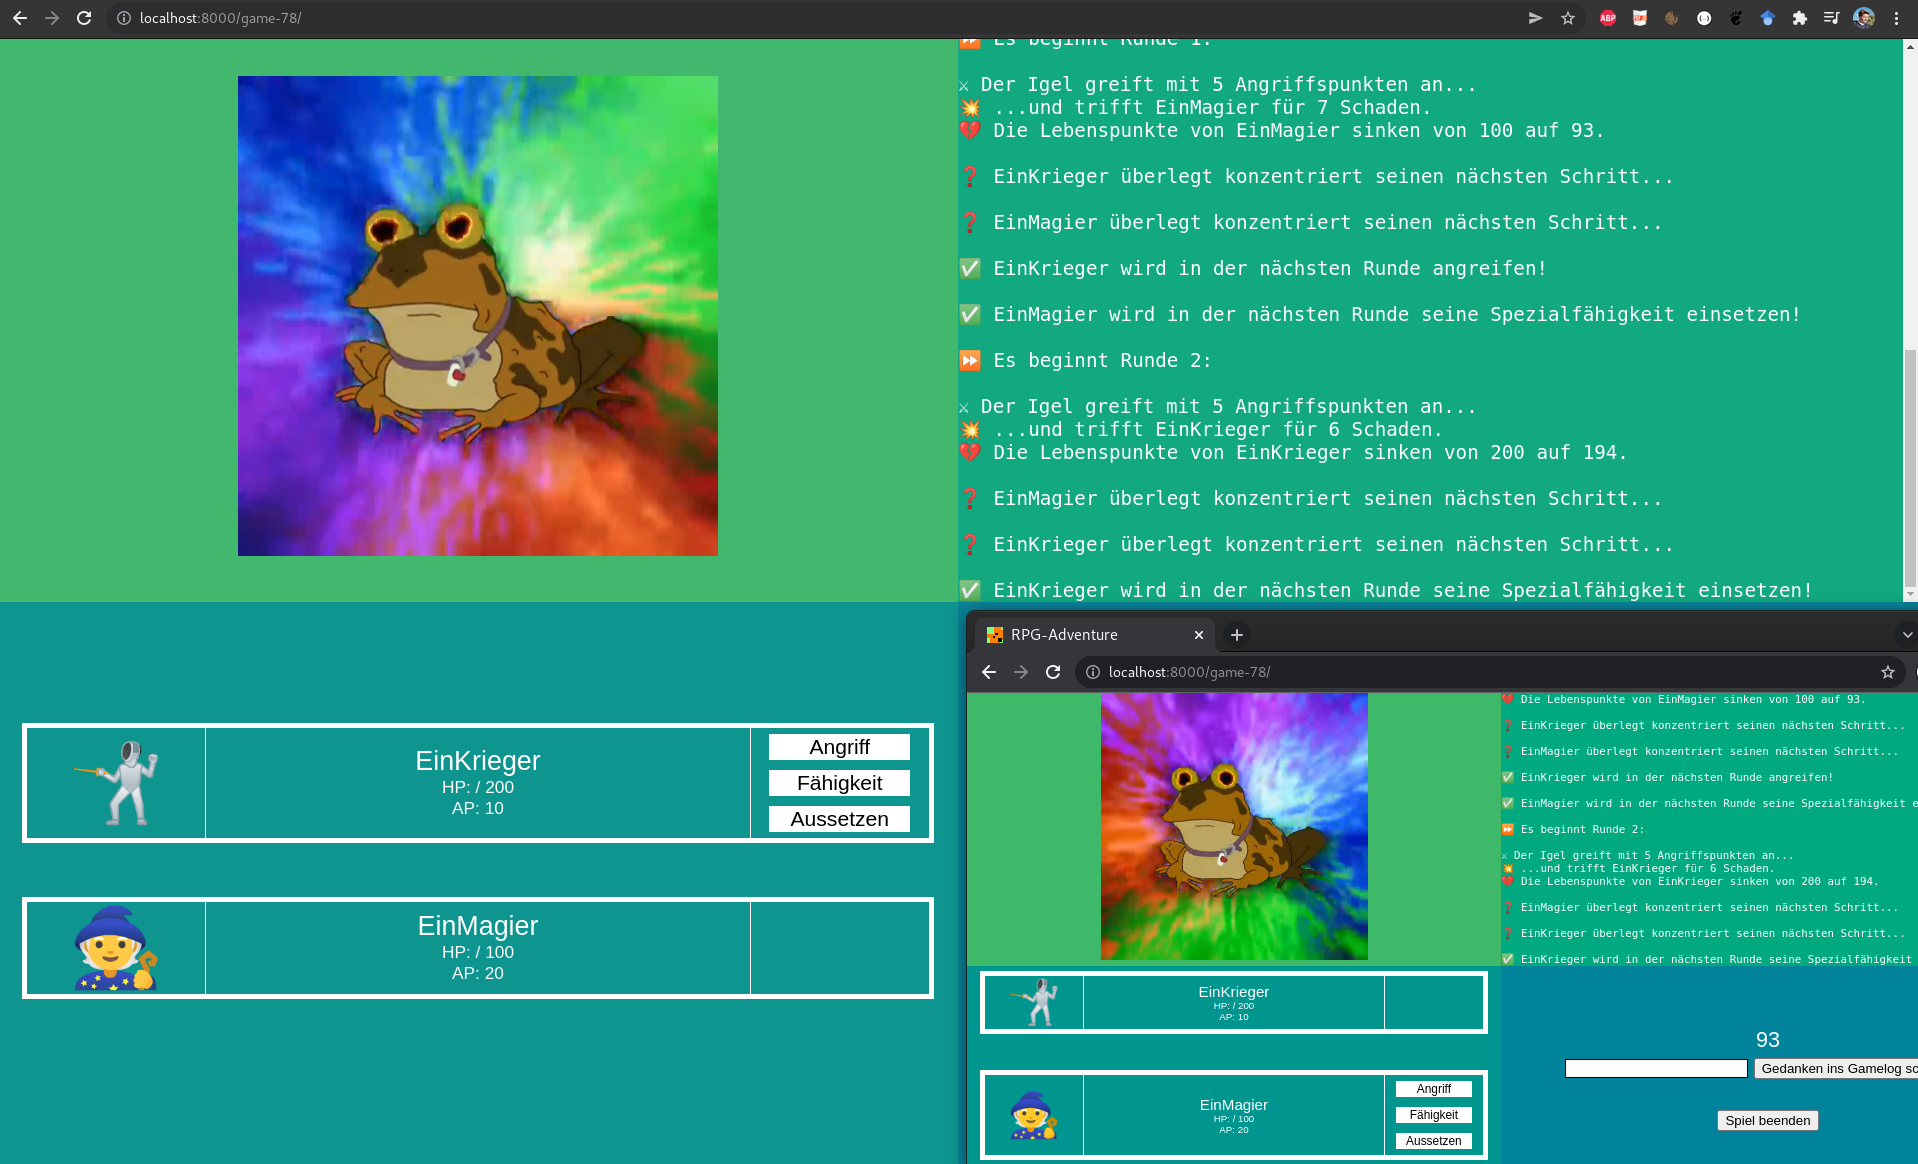
\includegraphics[width=0.7\textwidth]{2021-12-29-Bildschirmfoto-Entwicklungsstand-Runden-Status-400.png}
    \end{figure}

    \item Die Chatfunktion wurde implementiert. Hier jedoch abweichend vom Plan direkt als Meldungen im Game-Log und nicht in einem gesonderten Chat-Log und Chat-Fenster. Julian war damit im kurzen Teams-Gespräch gestern einverstanden. Den Aufbau der Game-Seite entsprechend angepasst und dem Game-Log deutlich mehr Raum eingeräumt. Außerdem weitere Anpassungen am Design und Style (Commit \url{https://git.io/JyDRK}).

\end{itemize}


\subsection{Entwicklung, Donnerstag 30.12.2021:}

Abschließender Schritt in der Implementation der Rundenlogik:

\begin{itemize}
    \item Die Schadensfunktion für Spieler wurde eingebaut: Damit kann dem Gegner nun Schaden zugefügt werden. Außerdem Prüfung auf Tod des Gegners incl. entsprechender Medlung (Commit \url{https://git.io/Jy9E7}).
\end{itemize}

Offen sind nun als nächste Schritte noch:
\begin{enumerate}
    \item Fähigkeiten der Spieler in Rundenlogik implementieren.
    \item Abschlussbildschirm für Sieg und Gameover konzeptionieren und implementieren. 
    \item Charakterentwicklung bei Sieg implementieren.
    \item Erweiterung der Infrastruktur aus Scripten, Anleitungen und des Git-Repos hin zum laden eines Default-Datensatzes (JSON-Datei) mit nutzbaren Spieldaten (insbesondere für Testzwecke und Nutzungen durch Dritte).
\end{enumerate}


\subsection{Entwicklung, Freitag 31.12.2021:}

Abarbeiten der zuletzt genannten, nächsten Schirtte. Hier: 

\begin{itemize}
    \item Die Charakterentwicklung wird mit Erfahrungspunkten gelöst: Durch Aktionen im Spiel bzw. Kampf (Schaden bekmmen, Schaden austeilen, Fähigkeiten nutzen) bekommen die entsprechenden Charaktere sofort entsprechende Erfahrungspunkte gutgeschrieben. Wird das Spiel gewonnen, werden alle von allen teilnehmenden Spielern in dieser Runde erspielten Erfarungspunkte noch einmal verdoppelt und jedem der Spieler gutgeschrieben. Verwendet werden können diese Erfahrungspunkte dann in der Charakteransicht um damit z.B. Lebenspunkte (HP) oder Angriffspunkte (AP) zu erhöhen (Commit \url{https://git.io/Jy7gl}).
\end{itemize}


\subsection{Entwicklung, Samstag 01.01.2022:}

Nach kurzer Abstimmung und Vorstellung meiner Ergebnisse bei Julian, letzte Anpassungen bzw. Entwicklungen: 

\begin{itemize}
    \item Ausgabe der erhaltenen XP beschleunigt: Es werden nun immer 10\% (aufgrundet auf die nächste Ganzzahl) der XP ausgegeben (Commit \url{https://git.io/JSTIq}).
    \item Einbau der Charakter-Fähigkeiten (Commit \url{https://git.io/JSkKJ}):
    \begin{itemize}
        \item Priester: Gruppe heilen=Alle HP erhöhen
        \item Zauberer: Schaden der Gruppe erhöhen=Alle AP erhöhen
        \item Krieger: Gegner blocken=AP Gegner verringern
    \end{itemize} 
    Damit die Fähigkeiten über mehrere Runden wirken können, musste eine Hilfstabelle angelegt werden: "AbilitysToApply". Hieraus werden zum Rundenwechsel die jeweils anzuwendenden Fähigkeiten gelesen und auf die relevaten Zahlen gewirkt. 
    \item Beispieldaten hinzugefügt und automatisches laden in die Datenbank über die local/dev-Skripte eingefügt (Commit \url{https://github.com/tstsrv-de/rpg/commit/1bfa99e89ddf2dbe817bdee2c870d1ddbe4f23c1}).
\end{itemize} 


\subsection{Entwicklung, Sonntag 02.01.2022}

Ein kurzer Anwendungstest mit einem versierten RPG-Spieler und IT-affinen Nutzer. Notizen dazu: 

\begin{itemize}
    \item Hinweis beim betreten der Lobby, dass das Spiel erst startet, wenn man einen "Platz-belegt" hat. 
    \item Man versuchte die Interaktion mit dem Spiel per Textkommandos über die Chatzeiel. Ineteresannte Alternative zur Nutzng der Buttons. 
    \item Der erste Level ist mit über 10 Runden deutlich zu lang und muss verkürzt werden.
\end{itemize}



\section{Noitzen für Reflektion}

\subsection{Rundenbasierter vs. chaotischer Spielablauf}

Der Ansatz die Entwicklung durch den Einsatz eines rundenbasierten Ablaufs bzw. Kampfsystems deutlich zu vereinfachen, muss wohl nach den Entwicklungen vom 27.12.2021 (\ref{ref-runden-impl}) zumindest angezweifelt werden. Denn der Aufwand, der durch die dadurf notwendige Konzeptionierung und Detailplanung entsteht ist nicht zu unterschätzen. Demengegen stünde bei einem chaotischen Spielablauf lediglich das Handling der Events. 

\subsection{Kleinteilige Aufgabenpakete} 

In der Entwicklung eine überschaubare Anzahl an kleinteiligen bzw. Teilufgaben vor sich zu haben, empfinde ich als sehr hilfreich. Man hat damit einen Überblick über die Arbeit der nächsten Tage. Bei der Entwicklung der Rundenlogik hatte ich durch die Kenntniss um die nächsten Runden-Schritte hier einen guten Überblick. Der Abschluss jeder einzelnen Teil-Aufgabe sorgte da laufend für postive Motivation. 
Ich vermute, dass dieser Effekt sehr ähnlich bei den agilen Methoden zum tragen kommt und zur Motivation genutzt wird. 

\subsection{Stichwortsammlung für Refektion}

\begin{itemize}
    \item Projektaufteilung: So abstimmen, dass verschiedene Arbeitsschritte gleichzeitig von verschiedenen Personen bearbeitet werden können.  
    \item Lernkurve und Codequalität: Eigentlich müsste man am Ende eines Projektes stets noch einmal von Vorne anfangen. Allein um alles zu korrigieren bzw. anzupassen, was im Projektverlauf gelernt wurde.
\end{itemize}


\section{Ideen für Erweiterungen über diese Projektarbeit hinaus}

Da der Umfang dieser Projekt beschränkt ist, können nicht alle erdachten Funktionen umgesetzt werden. Einige Ideen, sollen aber nicht ungenannt bleiben: 
\begin{enumerate}
    \item Würfel bei Schaden bzw. Angriff implementieren.
    \item Aggrotabelle und verbundene Funktionen implementieren.
    \item Transfer von Konstanten aus dem Code in eine Hilfstabelle für leichtere Anpassbarkeit später. Beispiele: \begin{itemize}
        \item Lebenspunkte und Angriffspunkte neuer Charaktere
        \item Faktoren bei der Berechnung von Erfahrungspunkten
        \item Faktoren bei der Berechnung des Schadens
    \end{itemize}
    \item Inaktive und getrennte Spieler bzw. Nutzer aus den Chatfunktionen der Weltkarte und Lobby entfernen. Ggfls. auch einen Timer für das Spiel anlegen der anderen Spielern anzeigt, wenn ein Spieler inaktiv bzw. getrennt vom Server ist. 
    \item E-Mail Funktion von Django konfigurien, damit das Zurücksetzen von Passwörtern u.A. möglich wird.
\end{enumerate}



	% 




\section{Aufgabenbeschreibung}
Beispielinhalt und Texte:
Das Thema der Seminararbeit gründet als Idee vor allem aus den folgenden beiden Beobachtungen aus privatem Lebensalltag und beruflicher Praxis: 
\begin{enumerate}
	\item Die seit den 2010er Jahren aufkommenden \textbf{smarten Technologien} finden im öffentlichen Raum und im Lebensalltag breiter Bevölkerungsschichten immer mehr Einzug. Drei Anwendungsbeispiele verdeutlichen und belegen das: 
	\begin{itemize}
	 \item Smart Watch: Uhren die z.B. um Fitness- und Nachrichtenfunktionen erweitert sind.
	 \item Smart TV: Fernsehgeräte die z.B. Zugriff auf Internet-Mediatheken erlauben.
	 \item Smart Home: Hausautomatisierungen und -steuerungen im privaten Bereich für  z.B. Licht und Heizung.
	 \end{itemize}

	 \item Das Aufkommen und der Erfolg der \textbf{PropTech\footnote{Kofferwort, englisch, aus 'property' (Immobilien) und 'technology' (Technologiegen)}-Branche} sowie die dieser Branche zuzuordnenden Unternehmen belegt die Relevanz von Innovation für die Wohnungswirtschaft ebenso wie die folgenden Erkenntnisse einer Studie \parencite[S. 18]{zia}:
	 \begin{itemize}
		 \item 72\% der befragten immobilienwirtschaftlichen Unternehmen nehmen Effizienzsteigerungen in Kernprozessen durch Einsatz digitaler Technologien an.
		 \item Weiter: Über ein Drittel gehen davon aus, dass Neugeschäft durch Einsatz digitaler Technologien generiert werden kann. 
	 \end{itemize}
\end{enumerate}

Vorgenannte Beobachtungen führen zu folgender Hypothese:

 \Rightarrow \textbf{Der Einsatz von smarten Displays in Quartieren der \ac{WoWi} ist möglich, wirtschaftlich und innovativ.}



\subsection{Was ist das Ziel der Projektarbeit?}
Beispielinhalt und Texte:
Als mögliche Standorte ergeben sich in Anlehnung an bisher übliche \glqq{}schwarze Bretter\grqq{} und \glqq{}Schaukästen\grqq{} in den Gebäuden sowie auch im Außenbereich vorhandenen Anlagen (Schaukästen, Werbeanlagen) auch für smarte Displays einige Vor- und Nachteile (Pro und Contra) die wie folgt stichpunktartig beschrieben werden: 

 \begin{itemize}
	 \item \textbf{Innenbereich:} 
	 \\ Wandmontage ebenso wie üblich und bekannte Schaukästen und schwarze Bretter im Windfang oder dem Etagenflur im Erdgeschoss eines Mietshauses.\\
	 \textbf{Pro:}\\
	  - Weiternutzung vorhandener, bewährter Montageorte \\
	  - Baurechtlich genehmigungsfrei \\
	  - Anbindung an Strom und Internet leichter als im Außenbereich \\
	  - Günstigere Bauart (kann weniger witterungsfest und vandalismussicher sein)\\
	 \textbf{Contra:}\\
	  - Wird wenig innovative Bauart zur Folge haben\\
	  - Kleinere Anzeigeflächen \\
	  - Nutzerkreis umfasst nur Mieter und Besucher des Hauses
	 \item \textbf{Außenbereich:} 
	 \\ Als freistehende Installation vor einem Wohngebäude, an einem markanten Wegepunkt im Quartier oder einem Innenhof eines Gebäudekomplexes.\\
	 \textbf{Pro:}\\
	  - Höhere Sichtbarkeit und Reichweite (nicht nur Mieter und Besucher eines Hauses, sondern auch Umfeld, Nachbarn und Durchgangsverkehr)  \\
	  - Attraktive Bauarten möglich \\
	  - Eröffnet weitergehende Nutzungsmöglichkeiten \\
	 \textbf{Contra:}\\
	  - Höhere Investitionskosten durch dem Standort geschuldete Bauart und Größe \\
	  - Erdarbeiten werden in der Regel nötig sein (Stromanschluss)  \\
	  - Baurechtlich genehmigungspflichtig, verursacht Mehrkosten und Aufwand
	  \item \textbf{Übergangsbereich Hauseingangstüre:} 
	  \\ Anbringung an Flächen die das Gebäude und den Außenbereich verbinden, beispielhaft genannt hier: Seitenteil der Türelemente im Hauseingangsbereich.\\
	  \textbf{Pro:}\\
	   - Unter Umständen umsetzbar als Modernisierungsmaßnahme (Nutzung als Videogegensprechanlage)  \\
	   - Technikaverse Bewohner und Besucher kommen zwangläufig in Kontakt mit dem smart Display \\
	  \textbf{Contra:}\\
	   -  Vorteile ergeben sich z.T. nur in noch nicht modernisiertem Bestand \\
	   -  Kleinerer Nutzerkreis und Anzeigefläche \\
 \end{itemize}

Eine weitergehende Bewertung oder Befürwortung einzelner Standorte soll hier nicht erfolgen um einzelne Anwendungsfälle nicht hier schon auszuschließen.


\subsection{Worin bestehen die (wahrscheinlichen) Herausforderungen? (allg. technisch und auch persönlich)}
Beispielinhalt und Texte:
Der Begriff soll daher hier geschärft werden um in der weiteren Verwendung un­miss­ver­ständ­lich zu sein.  

Die Definition erfolgt unter Bezug auf
\begin{enumerate}
	\item  die erfolgte Abgrenzung in 'enge' und 'weite' Definition nach \citeauthor{wirtschaftsfaktorimmo} (\citeyear[S. 9]{wirtschaftsfaktorimmo}) sowie
	\item die institutionelle Systematisierung der Immobilienwirtschaft nach \citeauthor{brauer2011einfuhrung} (\citeyear[S. 26]{brauer2011einfuhrung}).
\end{enumerate}

Die daraus entnommenen Zitate sollen hier im weiteren als gültige Definition für den verwendeten Begriff \textbf{Wohnungswirtschaft (WoWi)} gelten:  
\begin{itemize}
	\item Aus \citeauthor{wirtschaftsfaktorimmo} (\citeyear[S. 9]{wirtschaftsfaktorimmo}): \glqq{}alle Unternehmen, die an der Bewirtschaftung, Vermittlung und Verwaltung von Immobilien unmittelbar beteiligt sind\grqq{}. 
	 \item Sowie nach \citeauthor{brauer2011einfuhrung} (\citeyear[S. 36]{brauer2011einfuhrung}) zu den unterschiedlichen Rechtsformen \glqq{}(...)kommunalen, genossenschaftlichen und privaten Unternehmen(...)\grqq{} und den gleichwohl identischen Aufgabenfeldern: \glqq{}(...)nachhaltige Vermietung und Bestandsmanagement(...)\grqq{}.
\end{itemize}





\newpage
\section{Anforderungen}
Beispielinhalt und Texte:
Die genaue Zuordnung stellt sich also wie folgt dar:

\begin{table}[H]
	\caption{Zuordnung der Anforderungen der Hypothese zu den kritischen Anforderungen des Proof of Concept (PoC)}
	\label{tbl:zuordnungHypothesePoc}
	\begin{tabularx}{\textwidth}[ht]{|l|c|X|}
	\hline
	\textbf{Anforderung der Hypothese} & \textbf{Zuordnung} & \textbf{Abbildung in \ac{PoC}} \\
	\hline\hline 
	ist möglich & \Leftrightarrow & Prüfung der Machbarkeit  \\
	\hline 
	ist wirtschaftlich & \Leftrightarrow &  Effizienz-Faktoren aufzeigen \\
	\hline 
	ist innovativ & \Leftrightarrow &  Nutzbarkeit und Anwendungsfälle \\
	\hline
	\end{tabularx}
\end{table}


\subsection{Welche Techniken/ Technologien sollen eingesetzt werden, um die Aufgabe zu lösen/ realisieren?}
Beispielinhalt und Texte:

Eine Betrachtung der Wirtschaftlichkeit einer Einzelinvestition in ein smart Display in einem Quartier könnte damit nach z.B. folgendem Schema erfolgen:


\begin{table}[H]
	\caption{Mögliches Schema einer Wirtschaftlichkeits- und Effizienzbetrachtung der Einzelinvestition in smart Displays}
	\label{tbl:SchemaWBsmartDisplay}
	\begin{tabularx}{\textwidth}[ht]{cl}
	\hline
	\textbf{ - }   &  Investitionskosten (der Einzelmaßnahme) \\
	\textbf{ - }   &  lfd. Betriebs- und Wartungskosten  \\
	\textbf{ + }   &  lfd. Einsparung Personalkosten  \\
	\textbf{ + }   &  Refinanzierung als Modernisierungsmaßnahme   \\
	\textbf{ + }   &  Umlage von (Teilen der) Betriebskosten auf Gebäudenutzer  \\
	\textbf{ + }   &  Mehrerlöse durch Überlassung als Werbefläche an Dritte  \\
	\hline\hline
	\textbf{ = }   &  \textbf{in Euro messbare Wirtschaftlichkeit} \\
	\textbf{ + }   &  Digitalisierung eines Geschäftsprozesses  \\
	\textbf{ + }   &  Imagegewinn für das Quartier \\
	\textbf{ + }   &  Öffentlichkeitswirksame Einführung und Realisierung  \\
	\hline\hline
	\textbf{ = }   &  \textbf{gesamt zu bewertende Effizienz} \\
	\hline
\end{tabularx}
\end{table}

Kommt man nun zurück auf die Definition des Bergriffs der Effizienz nach \citeauthor{eichhorn2016} (\citeyear[S. 183 f.]{eichhorn2016}), kann man feststellen, dass es für die Beurteilung wesentliche Faktoren gibt, die nicht der Wirtschaftlichkeit zuzurechnen sind.



\subsection{Warum sollen gerade diese eingesetzt werden?}
Beispielinhalt und Texte:
Mit smarten Displays sind in dieser Seminararbeit nicht die von Desktop-Computer abnehmbaren und tragbaren LCD-Monitore gemeint die 2002 im Zusammenhang mit Microsofts Betriebssystem \glqq{}Windows CE for Smart Displays\grqq{} vorgestellt wurden \parencite{heise-ms-sd} und im Jahr 2004 wieder eingestellt worden sind \parencite{ct-3-2004}. 

\begin{figure}[H]
	\caption{Handteil eines smart Displays nach Microsoft-Konzept}\label{fig:HandteilMSsmartDisplay}
	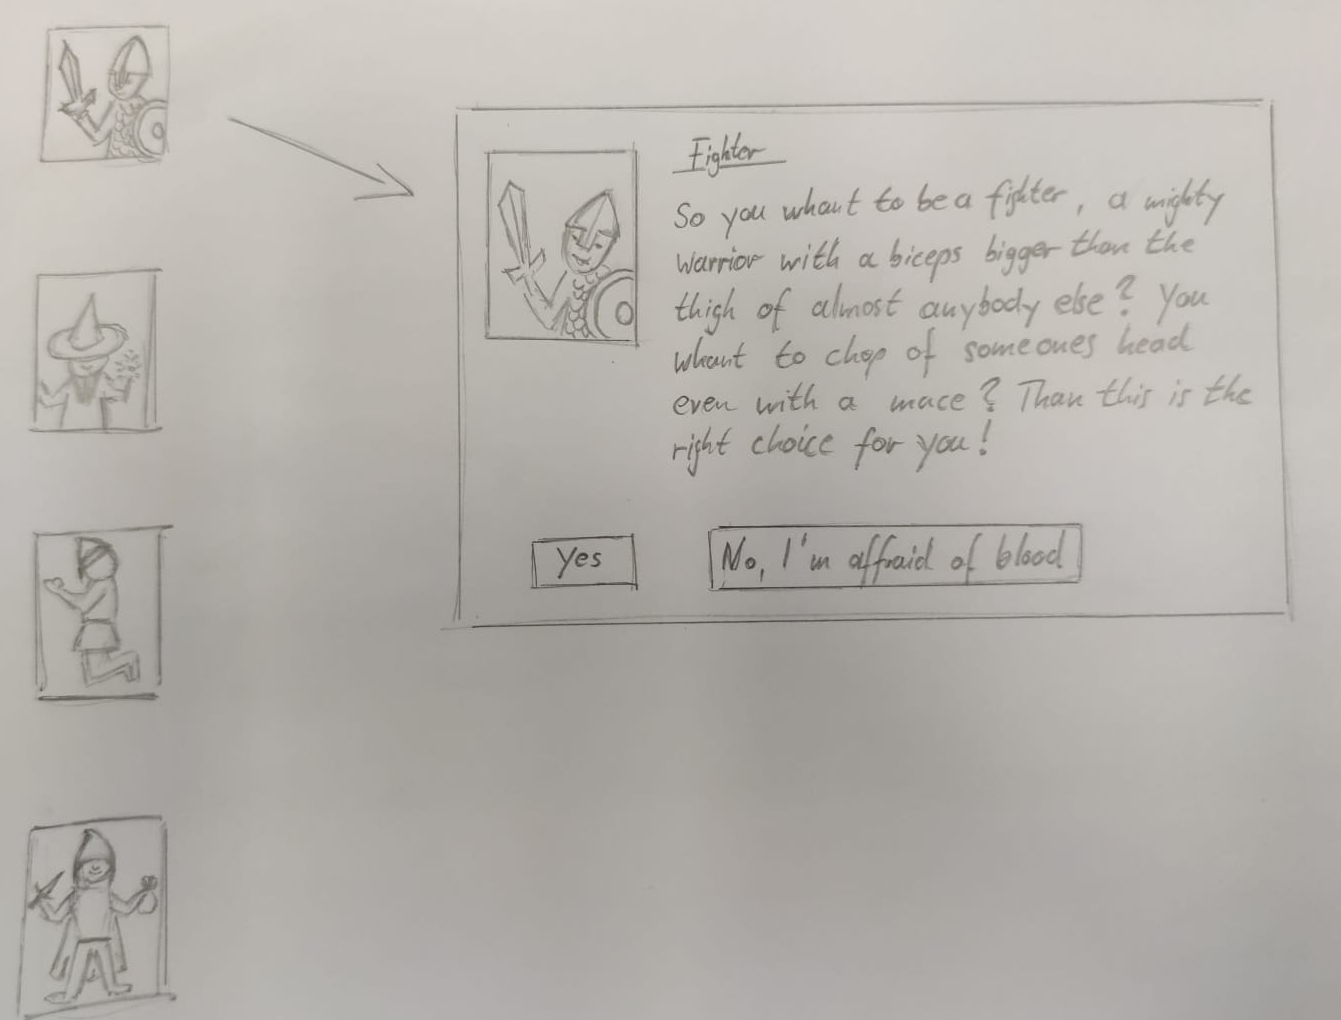
\includegraphics[height=5cm,keepaspectratio]{2021-11-29-Entwurf-Klassen-Ui}
	\\
	Quelle: Homepage von Mark Strehlow, Senior Interaction Designer\\ im Projekt Mira (\href{https://msdo.us/Microsoft-Mira}{msdo.us/Microsoft-Mira})
\end{figure}

Vielmehr sind hier erst noch durch Forschung und Entwicklung für die \ac{WoWi} zu schaffenden und nutzbar zu machenden Geräte gemeint.


\subsection{Gibt es besondere Anforderungen? (technisch, Benutzer, sonstige)}
Beispielinhalt und Texte:

\newpage
\section{Herangehensweise}
Beispielinhalt und Texte:

\subsection{Wie soll das Ziel erreicht werden (Vorgehen, Architektur)}
Beispielinhalt und Texte:

\newpage
\section{Vorstellung des Ergebnisses}
Beispielinhalt und Texte:

\newpage
\section{Reflektion}
Beispielinhalt und Texte:

 die Anwendung wird hier durch eine Betrachtung  der untenstehenden Punkte erfolgen: 
\begin{itemize}
	\item \textbf{Prüfung rechtlicher und IT-technischer Machbarkeit:}
	\\ Neben baurechtlicher Betrachtung hier auch Prüfung in Bezug auf verschiedenartige Realisierungen in Größe, Standort, Bauart und IT-Integration.
	\item \textbf{Aufzeigen und erörtern relevanter Effizienz-Faktoren:}
	\\ Umfasst typisch erwartbare Effizienz-Faktoren wie die Wirtschaftlichkeit ebenso wie auch darüber hinausgehende Auswirkungen die zur ebenso zur Effizienz zu zählen sind.
	\item \textbf{Darstellung möglicher Nutzbarkeiten und Anwendungsfälle:}
	\\ Ausführungen zu erwartbaren Einflüssen auf vorhandene Geschäftsprozesse in der \ac{WoWi} aber auch durch Aufzeigen von neuartigen und darüber hinausgehenden Anwendungsfällen und -bereichen.
\end{itemize}

Diese drei vorgenannten Punkte spiegeln die drei Anforderungen aus der Hypothese der Einleitung wieder und entsprechen dieser genau, in den jeweils genannten Reihenfolgen. 




\end{appendices}
\addtocontents{toc}{\protect\setcounter{tocdepth}{2}}






\newpage % Literaturverzeichnis

% Im Literaturverzeichnis "und" wieder durch "&" ersetzen	
	\DeclareDelimFormat*{finalnamedelim}{\addspace\&\space}

% Punkt hinter und vor der Jahreszahl entfernen	- Wichtig für Quell-Arten wie misc und online -- Sonst ein überflüssiger Punkt im LitVerz.
	\renewbibmacro*{author}{%
	\printtext{%
	\ifnameundef{author}
	{\usebibmacro{labeltitle}}
	{\printnames[apaauthor][-\value{listtotal}]{author}%
	\setunit*{\addspace}%
	\printfield{nameaddon}%
	\ifnameundef{with}
	{}
	{\setunit{}\addspace\mkbibparens{\printtext{\bibstring{with}\addspace}%
	\printnames[apaauthor][-\value{listtotal}]{with}}
	\setunit*{\addspace}}}%
	% \newunit\newblock%
	\usebibmacro{labelyear+extradate}}}

\printbibliography[heading=bibintoc,title=Literaturverzeichnis]

\newpage % Ehrenwörtliche Erklärung
\pagenumbering{gobble} % Keine Seitenzahlen mehr
\section*{Ehrenwörtliche Erklärung} 
	Hiermit versichere ich, dass die vorliegende Arbeit von mir selbstständig und ohne unerlaubte Hilfe angefertigt worden ist, insbesondere dass ich alle Stellen, die wörtlich oder annähernd wörtlich aus Veröffentlichungen entnommen sind, durch Zitate als solche gekennzeichnet habe. Weiterhin erkläre ich, dass die Arbeit in gleicher oder ähnlicher Form noch keiner Prüfungsbehörde/Prüfungsstelle vorgelegen hat. Ich erkläre mich damit \textbf{nicht einverstanden}, dass die Arbeit der Öffentlichkeit zugänglich gemacht wird. Ich erkläre mich damit einverstanden, dass die Digitalversion dieser Arbeit zwecks Plagiatsprüfung auf die Server externer Anbieter hochgeladen werden darf. Die Plagiatsprüfung stellt keine Zurverfügungstellung für die Öffentlichkeit dar.

			\par\medskip
			\par\medskip

			\vspace{5cm}

			\begin{table}[H]
				\centering
				\begin{tabular*}{\textwidth}{c @{\extracolsep{\fill}} ccccc}
					
					\myOrt, \the\day.\the\month.\the\year
					&
					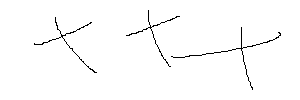
\includegraphics[width=0.35\textwidth]{unterschrift_rico}\vspace*{-0.35cm}
					\\
					\rule[0.5ex]{12em}{0.55pt} & \rule[0.5ex]{12em}{0.55pt} \\
					(Ort, Datum) & (Rico ) 
					\\

					
					  
					&
					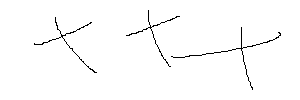
\includegraphics[width=0.35\textwidth]{unterschrift_henning}\vspace*{-0.35cm}
					\\
					 & \rule[0.5ex]{12em}{0.55pt} \\
					& (Henning ) 
					\\

					
					  
					&
					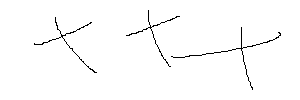
\includegraphics[width=0.35\textwidth]{unterschrift_julian.png}\vspace*{-0.35cm}
					\\
					 & \rule[0.5ex]{12em}{0.55pt} \\
					 & (Julian ) 
					\\



				\end{tabular*} \\
			\end{table}

\end{document}